% !TEX root = _main.tex

% ==========================================
% ここから本文．あとは各自で
% ==========================================

%1
\section{はじめに}\label{sec:hajimeni}

筆者は10年来「NEWS」というアイドルグループを応援し続けている．NEWSは2003年，旧ジャニーズ事務所から9人組グループとして結成し，紆余曲折を経て2020年から3人で活動を行っている．

長年のファン活動を通じた筆者の感触として，NEWSには\senaka \emotional という2つの重要なキーワードが関わっていると感じている．
公式アカウント\cite{NEWS_Chill}や過去に収録されたドキュメンタリー\cite{Ongaku}など様々な発信情報からこれらのキーワードを目にする機会も多く，NEWSのアイドルグループとしての魅力を表すにふさわしいものだと考えている．


%------ このへんは，キーワードを説明する 後の章にもっていく ------------------
%彼らを応援している中で，「NEWSは背中を押してくれる楽曲が多い」といった声を聴くことがあ\red{る}．そのような印象を持つ楽曲は2012年以降に発表された楽曲が多いと感じている．実際，公式アカウントでグループを紹介する際には「多くの人の背中を押してきた」\cite{NEWS_Chill}と書かれていた．ほかにも（音楽ドキュメンタリー）の中でメンバーが「エモーショナルさがNEWSの魅力になってきている」と発言しており（出典），そこに挙げられた楽曲はどれも2012年以降に発表されたものだった．

%エモーショナルとは「強く感情に訴えるさま」という意味がある（出典）。NEWSの場合この「感情に訴えるさま」が「背中を押す」感覚につながったのではないだろうか．

%「背中を押す」と聞くと応援歌というジャンルを思い浮かべるかもしれない．しかし、筆者はNEWSの楽曲に多いものが世間に定義される応援歌ではなくメッセージ性を強めた「メッセージソング」ではないかと考えた．応援歌とは「競技で味方の選手・チームを励ますためにうたう歌」（出典）という意味がある．NEWSにもバレーボール大会やサッカーワールドカップのタイアップ曲はあるがドキュメンタリー内でメンバーが挙げていた楽曲は含まれていなかった．このことから世間で定義される応援歌とNEWSが「背中を押してくれる」楽曲は別物であると考えられた．

%そしてメンバーが挙げた楽曲の紹介記事ではその楽曲を「メッセージソング」と表記していた（出典）．メッセージは「情報や意思を伝えるために送る文章や言葉のことを指す（出典）」という意味がある．このことからNEWS楽曲にある「背中を押す」感覚はメッセージソング由来であり，メッセージと言われるように，この感覚は楽曲にメロディーやリズムなどの要素がある中でも主に歌詞からの訴えが多くの人の心に響くことから生まれると考えた．
% ----------------------------------

一方で，20年以上の活動を経て，NEWSは過去に4回，グループの人数が減るタイミングがあった．
それだけの長期にわたる活動で，かつメンバー構成が変わるなどしていけば，徐々に楽曲の表現の傾向が変化していくのが自然であろう．特に2012年は，グループが4人体制になった年であり，前述のキーワードに象徴されるような楽曲が発表されるようになった時期でもある，

そこで本研究では，体制の変化に伴う楽曲の変化を，特に「メッセージ」や「背中を押す」に直結するであろう歌詞に着目して，活動21年の歴史で変化してきた歌詞傾向について探ることを目的とする．
%、人数時代別の歌詞の傾向，単語に着目した使用傾向の移り変わり，キーワードごとに選曲した楽曲内での単語を基にした使用傾向の移り変わりについて分析している．

%2
\section{NEWSの歴史}
%\begin{verbatim}
2003年9月15日，「バレーボールワールドカップ2003」のイメージキャラクターとしてNEWSは結成された．メンバーは森内貴寛，内博貴，草野博紀，錦戸亮，山下智久，手越祐也，小山慶一郎，加藤成亮，増田貴久の九人であった．
2003年11月7日に「NEWSニッポン」でCDデビューした後，メンバーの森内貴寛が同年12月に活動休止，その後脱退する．この期間を九人時代とする．\\
2004年5月に「希望〜Yell〜」でメジャーデビューを果たす．
その後約2年の活動の後2006年末までに内博貴，草野博紀が脱退する．この期間を八人時代とする．\\
約1年の活動休止期間を経て2007年から6人で活動を再開した．
約5年半の活動期間をもって2011年10月に山下智久，錦戸亮が脱退する．この期間を六人時代とする．\\
約半年の活動休止期間を経て2012年4月から4人で活動を再開した．約8年間の活動期間をもって2020年6月に手越祐也が脱退する．
この期間を四人時代とする．\\
2020年6月から現在に至るまで3人で活動を行っている．この期間を三人時代とする．\\
以下\protect\tabref{tab:news-history}にまとめた年表を示す．\\
%\end{verbatim}

\begin{table}[h]
	\centering
	\caption{NEWS年表}
	\label{tab:news-history}
	\begin{tabular}{c|l|l}
		\hline
		人数 & いつ       & 出来事                       \\
		\hline\hline
		9  & 2003年9月  & NEWSが結成する．                \\
		   & 2003年11月 & 『NEWSニッポン』でインディーズデビューをする． \\
		   & 2003年12月 & メンバーの森内が活動休止，のちに脱退する．     \\
		\hline
		8  & 2004年5月  & 『希望～Yell～』でメジャーデビューを果たす．  \\
		   & ～2006年   & メンバーの内，草野が脱退する．           \\
		\hline
		6  & 2007年1月  & 約1年の活動休止を経て6人で活動を再開する．    \\
		   & 2011年11月 & メンバーの山下，錦戸が脱退する．          \\
		\hline
		4  & 2012年4月  & 約半年間の活動休止を経て4人で活動を再開する．   \\
		   & 2020年6月  & メンバーの手越が脱退する．             \\
		\hline
		3  & 2020年6月～ & 3人で活動をする．                 \\
		\hline

		%「表の中身を書く」
	\end{tabular}
\end{table}

%\begin{figure}[h]
%\centering
%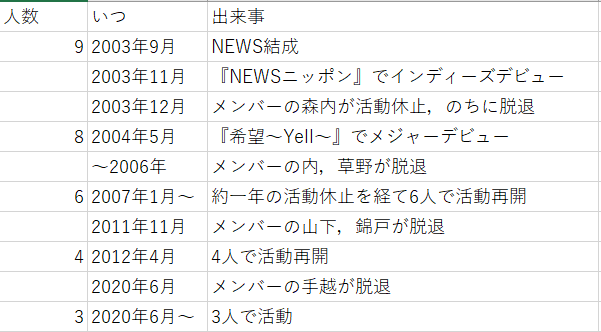
\includegraphics[width=\hsize]{fig/news_history.png}
%\caption{NEWS年表}
%\label{fig:news_history}
%\end{figure}

今回，NEWSの歴史を人数時代で区別し，それぞれの時代の特徴を歌詞の面から分析する．

1章で「グループの人数が変わると歌詞の傾向が変わっていくはずだ。」と，筆者が人数時代ごとに特徴が出ると思ったことには理由がある．それはNEWSが結果としてメインメンバーが脱退してきたからだ．\\
アイドルグループには人気などに基づいてグループの軸，センターを任される中心メンバーがいることが多く，またその中心メンバーに合わせた楽曲を作ることが多い．NEWSの場合，山下智久を中心に結成された歴史があり6人時代までは彼が中心にいた．それはシングルのジャケット写真から見ても明らかでありデビュー曲であるNEWSニッポン(2003)\cite{NEWSnippon}から6人時代最後の曲であるFighting Man(2010)\cite{FightingMan}までの14曲のうち彼がセンターもしくは上部，前方に置かれているものは13曲になる．\\
それほどまでに圧倒的な立ち位置にいた山下智久が脱退し4人になるタイミングではグループが解散する話も上がったが結果としてNEWSは4人で活動を再開し現時点では最も長い9年間の活動を行った．この間中心に据えられたのは手越祐也だ．彼も2020に脱退したのだが4人で活動を再開したチャンカパーナ(2012)\cite{Chankapana}からトップガン/Love Story(2019)\cite{LoveStory}までの12枚のシングルのうち彼がジャケット写真のセンターに置かれている曲は8曲になる．\\
このように直近で脱退したメンバーはNEWSにおいて中心メンバーといえる立ち位置にあり，彼らを中心に楽曲をリリースしていたとすると楽曲の傾向が大きく変わると考えられる．また，過去のドキュメンタリー\cite{Ongaku}内でメンバーが「エモーショナルさがNEWSの魅力になってきている」と発言しており,そこに挙げられた楽曲はどれも2012年以降に発表されたものだったのだが，これは4人の再始動の経緯と関係があると筆者は考える．先ほど述べたようにNEWSは6人から4人に代わるタイミングで解散の危機まで追い詰められた\cite{kysg}上に，山下智久の脱退直後は「イチゴのないショートケーキ」や「具のないおでん」とまで揶揄されていた．そこから再始動を果たすのだが，この一度どん底に落ちてから再始動したという背景の歴史があるからこそ，彼らが歌う曲のエモーショナルさがより引き出され，そして歌うことが増えた要因だと考えられる．\\

%加藤さんの発言「自分たちがもがいている姿を見せることで，人を励ますような歌に説得力が生まれることもあるかもしれない」は理由付けに使える気がする．


上記の理由からNEWSの楽曲は人数ごとに，特に6人時代から4人時代で大きく変化していると考え今回は歌詞に視点を当て傾向を分析することにした．



\section{分析目的と手法}

\subsection{分析のねらい}

本研究はNEWSが歌う楽曲の歌詞の特徴に着目し、デビューしてから21年の歴史で変化してきた歌詞傾向について探る．具体的には，大きく分けて二つの分析を行う．
一つは22年の活動期間での歌詞の移り変わり（第\ref{sec:years}章），もう一つは第\ref{sec:hajimeni}章で述べた2つのキーワード\senaka \emotional に合致する楽曲を絞った分析（第\ref{sec:words}章）を行う．



\subsection{対象楽曲と歌詞データ収集}
%まずはNEWSのどういう楽曲を扱うのか先に書く．
%著者がいつ集めたものかは読者には不要．NEWSのいつからいつまでの何曲をどうやってあつめたかを知らせるべし

%NEWS楽曲266曲(2024/11/13現在)

%分析において必要なのは＊＊＊で，どうやって集める
本研究の分析に際し，収集する必要のあるデータは「曲名」「発売日」「歌詞」「グループ人数」の４つである．
今回分析対象としたNEWS楽曲は歌ネット\cite{utanet}に基づいて収集した266曲(2024/11/13現在)である．


各楽曲に対しグループのメンバー構成時期と照合して，９，８，６，４，３のグループ人数を割り振った．
%グループ人数は，発売日に基づいて
%\figref{fig:news}を発売日順\footnote{NEWSニッポンアルバム\cite{nippon}に基づく}に並び変えたうえで人数時代別に9,8,6,4,3の番号を割り振った．NEWSニッポンアルバム収録時に発売日が合わせられていたため入れ替えている．%ここ意味不明

%\begin{figure}[b]
%	\centering
%	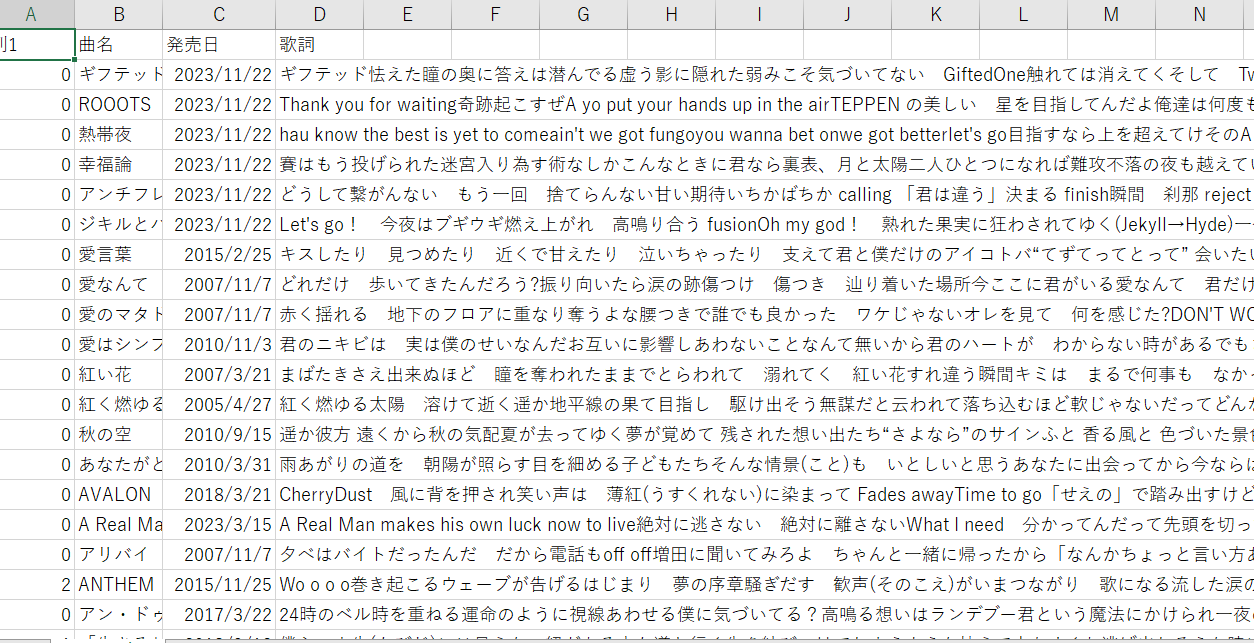
\includegraphics[width=\hsize]{fig/fig1.png}
%	\caption{NEWSの曲名，発売日，歌詞のデータ}
%	\label{fig:news}
%\end{figure}
%
%
%
%\begin{figure}[tb]
%	\centering
%	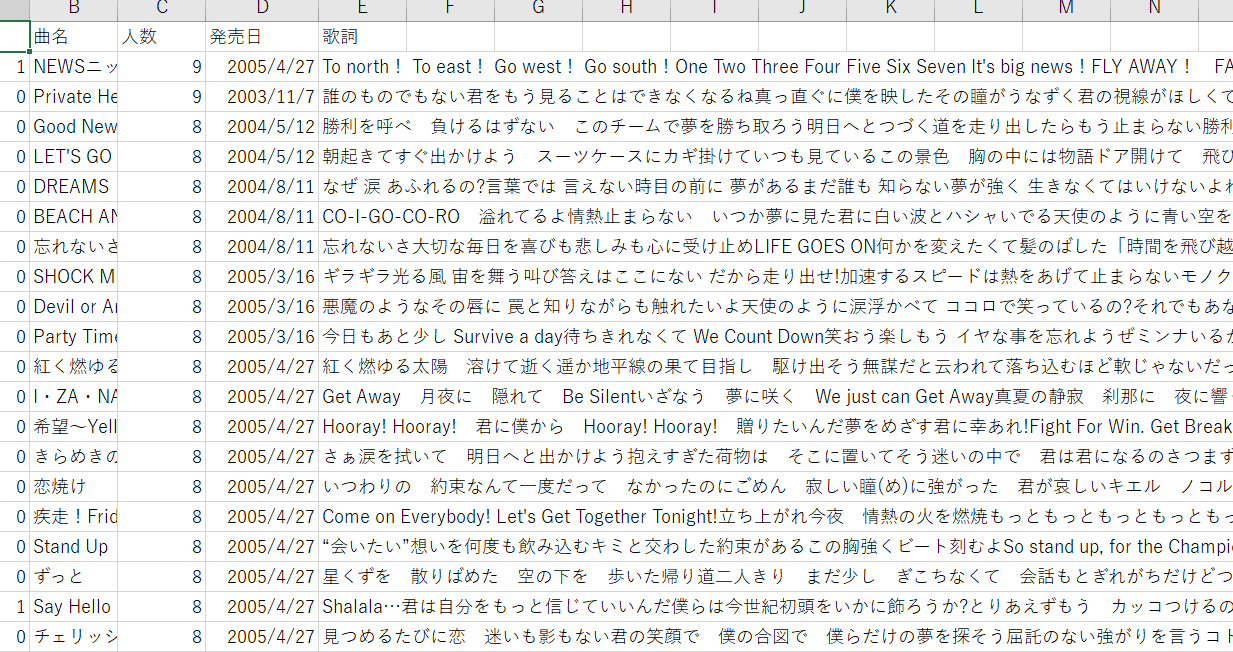
\includegraphics[width=\hsize]{fig/fig2.png}
%	\caption{図\ref{fig:news}に「人数」列を追加したデータ}
%	\label{fig:ninzu}
%\end{figure}

最終的に，グループ人数時代ごとに楽曲データを分割し，５つのファイルからなる歌詞データを用意した．
\figref{fig:3nin}に歌詞データの一部を示す．


\begin{figure}[b]
	\centering
	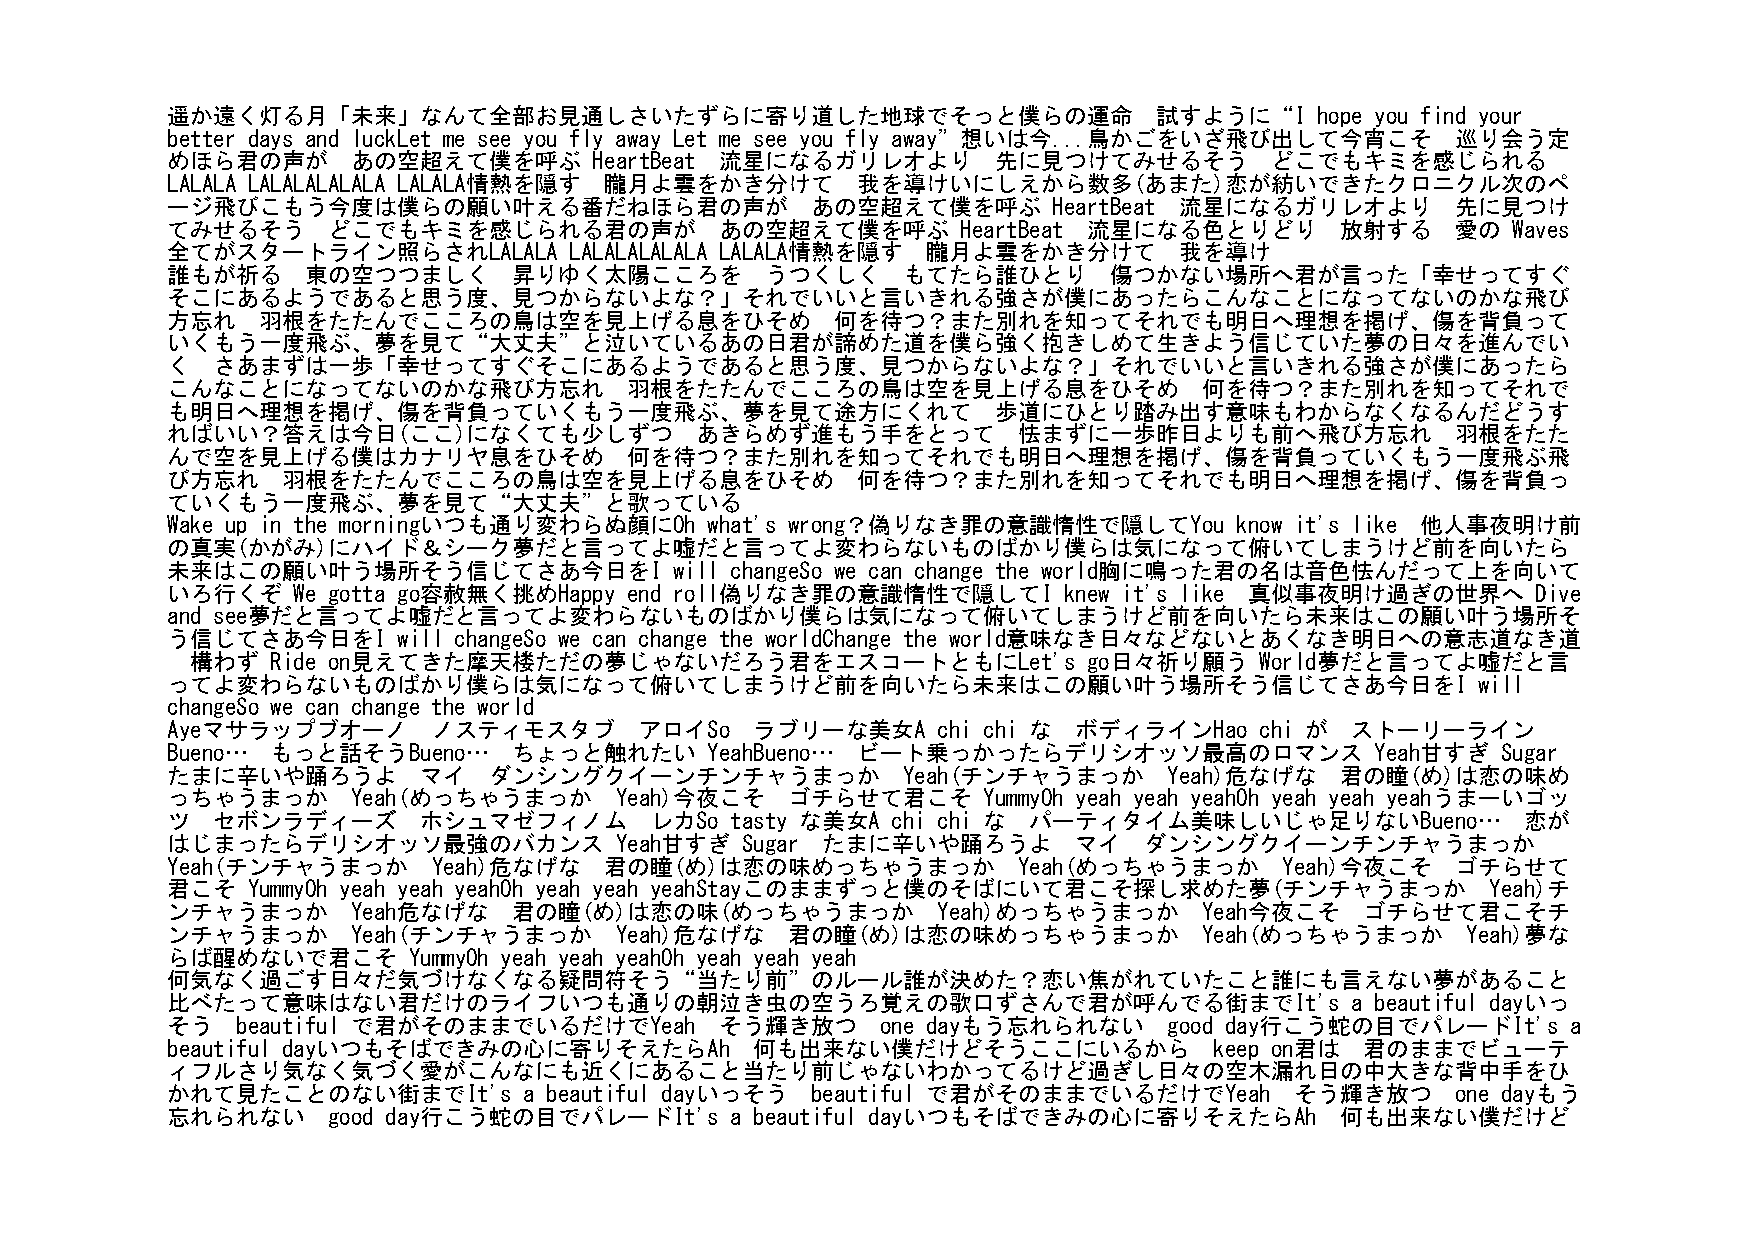
\includegraphics[width=\hsize]{fig/news_3.pdf}
	\caption{3人時代楽曲の歌詞データ}
	\label{fig:3nin}
\end{figure}

%以上の手順で人数時代別の歌詞データを作成した

\subsection{歌詞の形態素解析}
作成した歌詞データに対してKH Coder)\cite{KHcoder}を使用し，分析を進めるためのデータ形成を行った．

KH Coderとは計量テキスト分析またはテキストマイニングのための自由ソフトウェアである．

KH Coderには「代名詞」「名詞」「サ変名詞」「形容動詞」「固有名詞」「組織名」「人名」「地名」「ナイ形容」「副詞可能」「未知語」「タグ」「感動詞」「動詞」「形容詞」「副詞」「名詞B」「動詞B」「形容詞B」「副詞B」「名詞C」「否定助動詞」「形容詞（非自立）」「その他」「HTMLタグ」の25種類に品詞が分類される．
本研究で品詞ごとに分析をする際に名詞と副詞に関しては筆者自身が意味のある語彙として感じた品詞をピックアップした．\\
品詞ごとの分析で今回使用したのは主に「代名詞」「動詞」「形容詞」「名詞」「サ変名詞」「形容動詞」「ナイ形容」「名詞B」「名詞C」「副詞可能」「副詞」「副詞B」の計12種の品詞とした．
{\protect\tabref{tab:hinshi}に今回使用した品詞をまとめている．

\begin{table}[h]
	\centering
	\footnotesize
	\caption{今回使用した品詞}
	\label{tab:hinshi}
	\begin{tabular}{c||c}
		\hline
		品詞  & 今回使用するKHcoderの分類          \\
		\hline
		代名詞 & 代名詞                       \\
		動詞  & 動詞                        \\
		形容詞 & 形容詞                       \\
		副詞  & 副詞可能，副詞，副詞B               \\
		名詞  & 名詞，サ変名詞，形容動詞，ナイ形容，名詞B，名詞C \\
		\hline

		%「表の中身を書く」
	\end{tabular}
\end{table}


%\begin{figure}[tb]
%	\centering
%	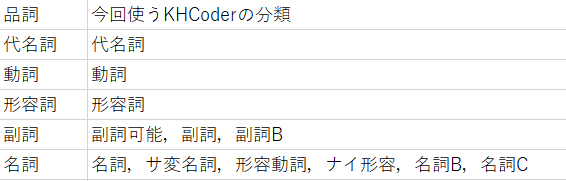
\includegraphics[width=\hsize]{fig/hinshi.png}
%	\caption{今回使用した品詞}
%	\label{fig:hinshi}
%\end{figure}

まず人数ごとにテキストファイルを読み込みKH Coder内の機能を用いて「使用回数」と「使用曲数」の2種類の表を出力した．
使用曲数の表は歌詞のリフレイン（繰り返し）に考慮したものとなっている．例えば「チャンカパーナ」という単語はNEWSの中で18回登場するがそのすべてが楽曲『チャンカパーナ』で歌われている．このように特定の単語を何度も歌うリフレインは使用回数に影響が出ると考え今回は二種類とも出力した．
出力した表にはすべての品詞が書き出されているがここから\tabref{tab:hinshi}をもとに名詞と副詞は複数種類をまとめて一つにした．
その後，品詞ごとに一つの表にまとめて個数とそれに基づく割合を求めた．
\figref{fig:shiyoukaisu_meishi},\figref{fig:shiyoukyokusu_meishi}に歌詞データの一部を示す．


\begin{figure}[tb]
	\centering
	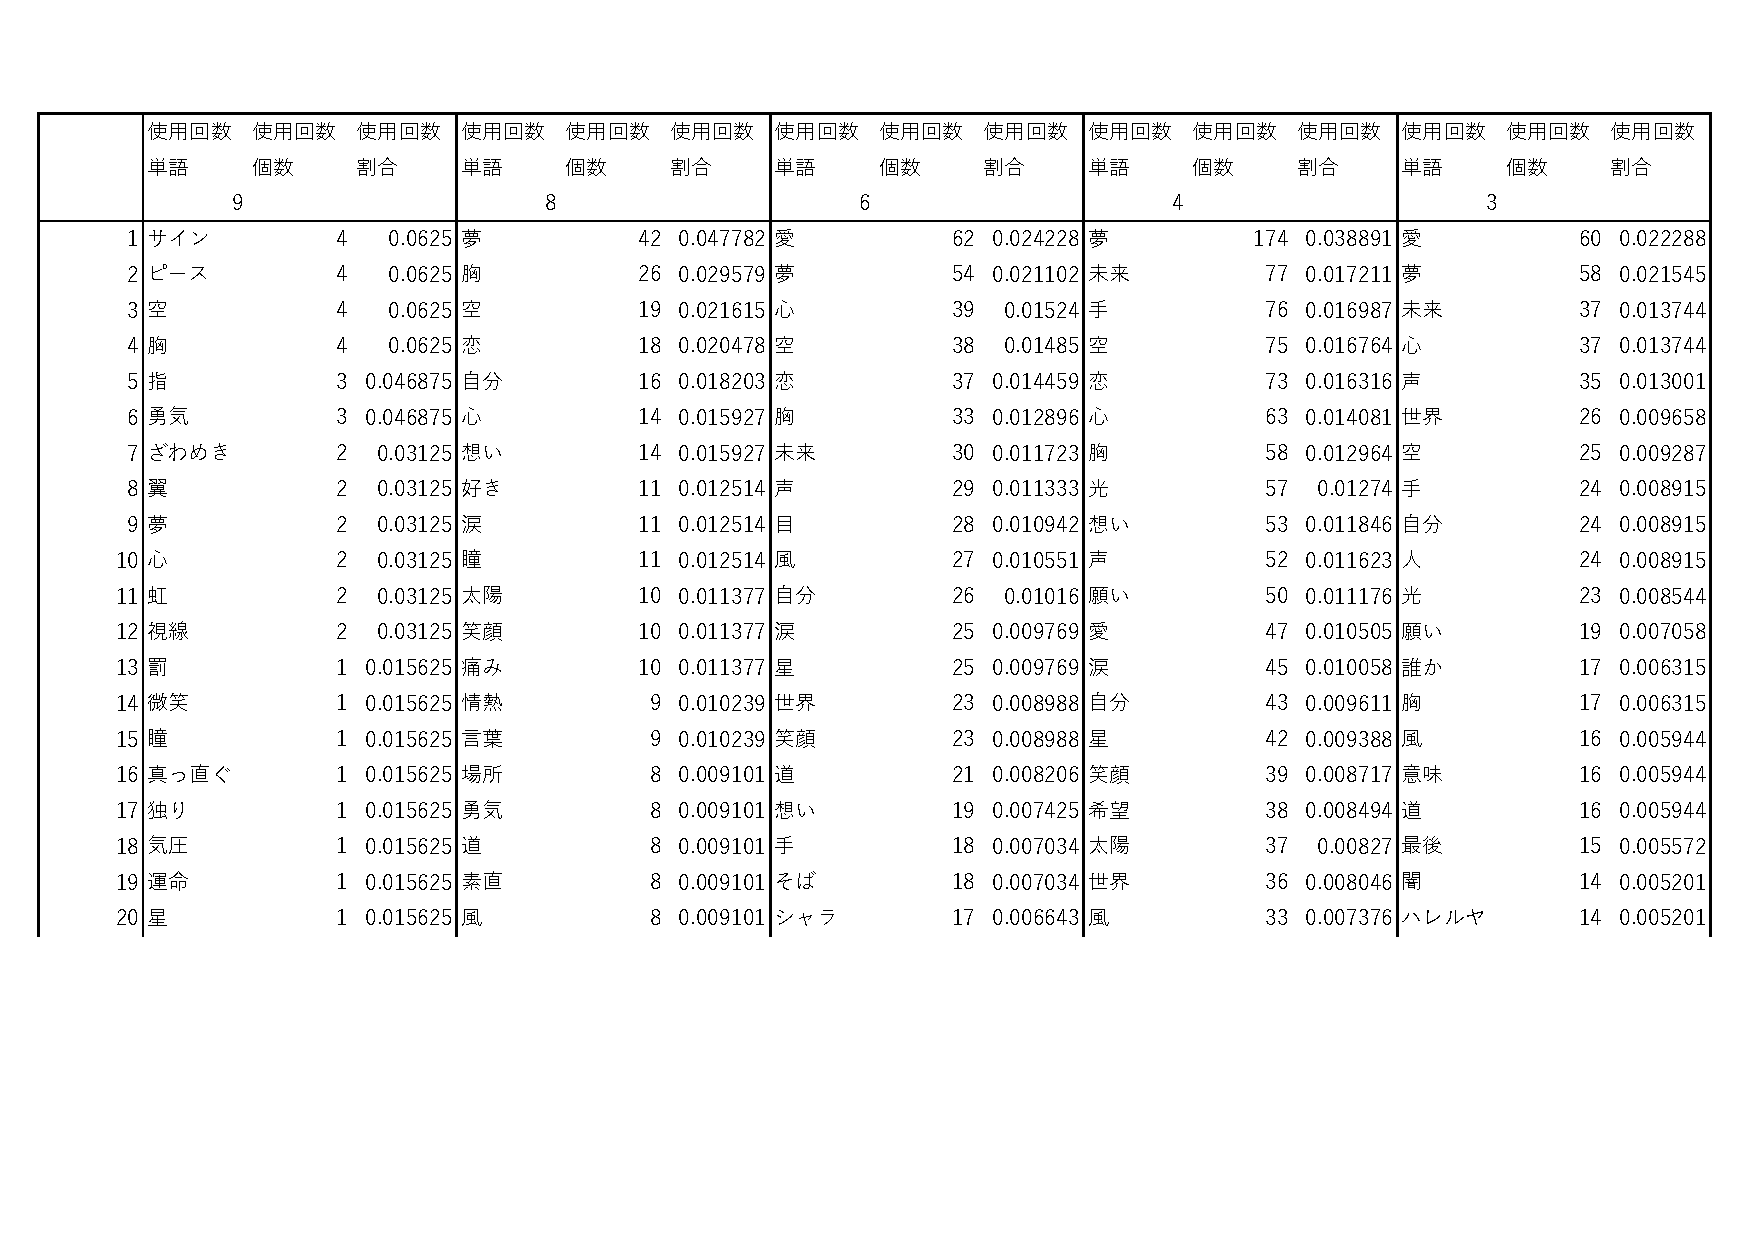
\includegraphics[width=\hsize]{fig/shiyoukaisu_meishi.pdf}
	\caption{使用回数をまとめた表の一部(名詞)}
	\label{fig:shiyoukaisu_meishi}
\end{figure}

\begin{figure}[tb]
	\centering
	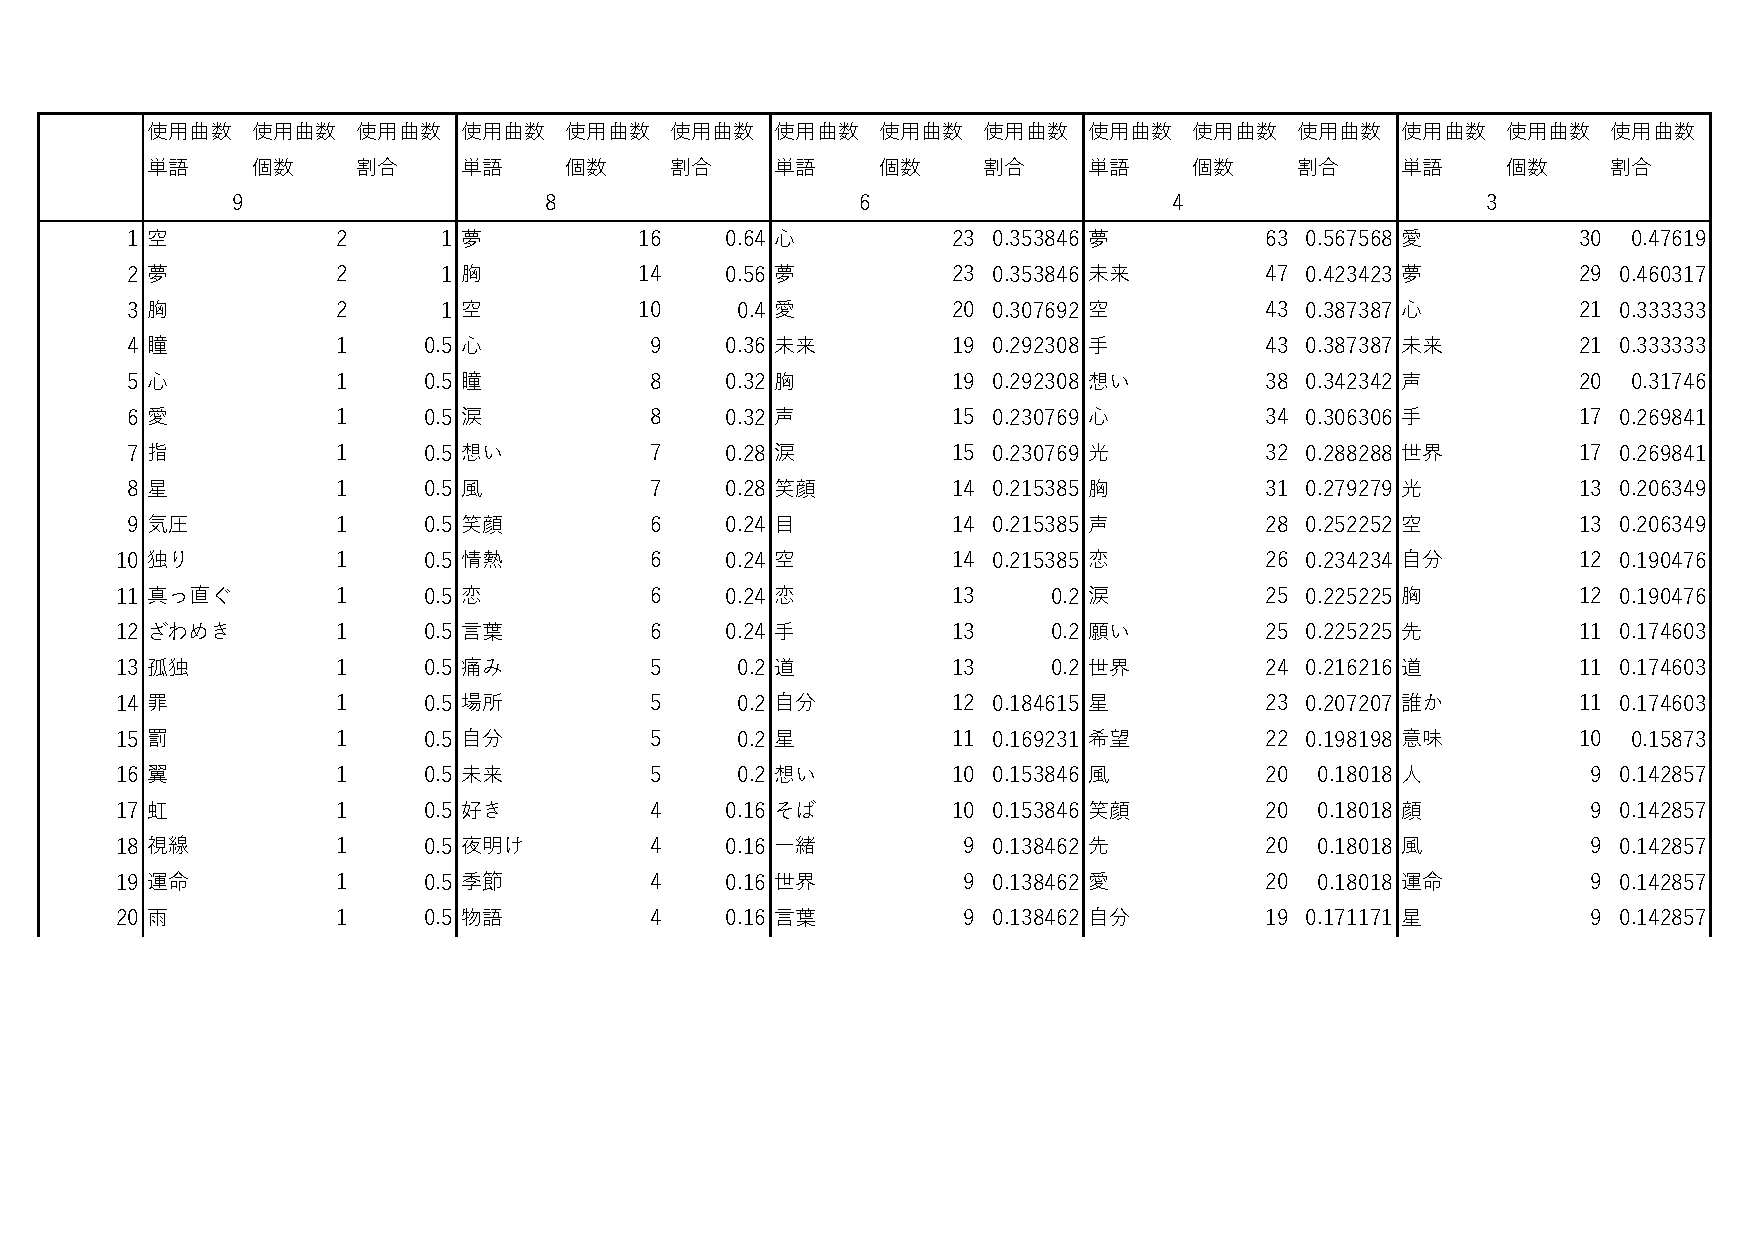
\includegraphics[width=\hsize]{fig/shiyoukyokusu_meishi.pdf}
	\caption{使用曲数をまとめた表の一部(名詞)}
	\label{fig:shiyoukyokusu_meishi}
\end{figure}


以上の流れでNEWS楽曲の時系列比較データを作成した．


\section{時代別の歌詞分析}\label{sec:years}
%ここではNEWSの歴史を人数時代で区別し，それぞれの時代の特徴を歌詞の面から分析する．

%1章で「グループの人数が変わると歌詞の傾向が変わっていくはずだ。」と，筆者が人数時代ごとに特徴が出ると思ったことには理由がある．それはNEWSが結果としてメインメンバーが脱退してきたからだ．アイドルグループには人気などに基づいてグループの軸，センターを任される中心メンバーがいることが多く，またその中心メンバーに合わせた楽曲を作ることが多い．NEWSの場合，山下智久を中心に結成された歴史があり6人時代までは彼が中心にいた．それはシングルのジャケット写真から見ても明らかでありデビュー曲であるNEWSニッポン(2003)\cite{NEWSnippon}から6人時代最後の曲であるFighting Man(2010)\cite{FightingMan}までの14曲のうち彼がセンターもしくは上部，前方に置かれているものは13曲になる．
%それほどまでに圧倒的な立ち位置にいた山下智久が脱退し4人になるタイミングではグループが解散する話も上がったが結果としてNEWSは4人で活動を再開し現時点では最も長い9年間の活動を行った．この間中心に据えられたのは手越祐也だ．彼も2020に脱退したのだが4人で活動を再開したチャンカパーナ(2012)\cite{Chankapana}からトップガン/Love Story(2019)\cite{LoveStory}までの12枚のシングルのうち彼がジャケット写真のセンターに置かれている曲は8曲になる．
%このように直近で脱退したメンバーはNEWSにおいて中心メンバーといえる立ち位置にあり，彼らを中心に楽曲をリリースしていたとすると楽曲の傾向が大きく変わると考えられる．また，過去のドキュメンタリー\cite{Ongaku}内でメンバーが「エモーショナルさがNEWSの魅力になってきている」と発言しており,そこに挙げられた楽曲はどれも2012年以降に発表されたものだったのだが，これは4人の再始動の経緯と関係があると筆者は考える．先ほど述べたようにNEWSは6人から4人に代わるタイミングで解散の危機まで追い詰められた\cite{kysg}上に，山下智久の脱退直後は「イチゴのないショートケーキ」や「具のないおでん」とまで揶揄されていた．そこから再始動を果たすのだが，この一度どん底に落ちてから再始動したという背景の歴史があるからこそ，彼らが歌う曲のエモーショナルさがより引き出され，そして歌うことが増えた要因だと考えられる．

%上記の理由からNEWSの楽曲は人数ごとに，特に6人時代から4人時代で大きく変化していると考え今回は歌詞に視点を当て傾向を分析することにした．

NEWS楽曲は全266曲分収集しているが各人数時代ごとに以下の楽曲数で分けられた．

\begin{itemize}
	\item 9人時代：2曲（613単語）
	\item 8人時代：25曲（6626単語）
	\item 6人時代：65曲（20165単語）
	\item 4人時代：111曲（34416単語）
	\item 3人時代：63曲(19455単語）
\end{itemize}


活動年数の差から必然的に曲数，単語数に差が生まれてしまう．しかし，その差も特徴の一つであると筆者は考えている．
今回の分析ではそのまま個数を出したものとは別に割合を求める分析がある．
ありのままのNEWSの特徴としてみる個数と時代ごとに比較できるように割合を求めたもの，この二つで比較を行う．

\subsection{ワードクラウドによる筆者が感じた第一印象}
ワードクラウドとは文章中で出現頻度が高い単語を複数選び出し，その頻度に応じた大きさで図示する手法\cite{wordcloud}のことである．今回はRを使用してワードクラウドから各時代の印象的な語彙を追っていく．\\
ワードクラウドにすることで視覚的に人数時代別の特徴をとらえたいと考えた．
今回は使用回数のみに焦点を当て，単語は名詞，形容詞，動詞であり，そのうちカギかっこや記号などを除いて上位150単語を出している．
以下それぞれの時代のワードクラウドを示す．


\begin{figure}[tb]
	\centering
	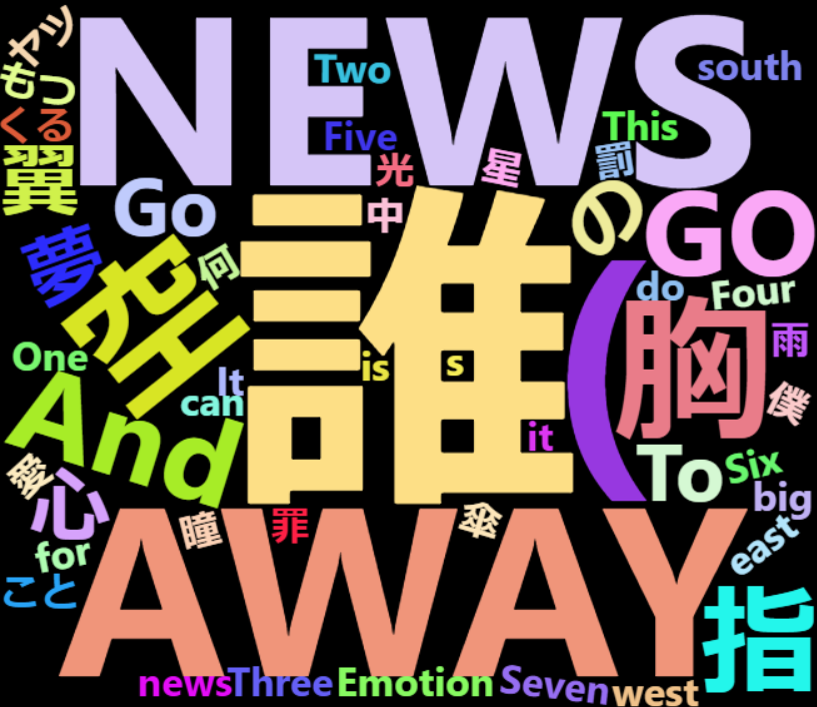
\includegraphics[width=\hsize]{fig/wc9.png}
	\caption{９人時代}
	\label{fig:wc9}
\end{figure}
\begin{figure}[tb]
	\centering
	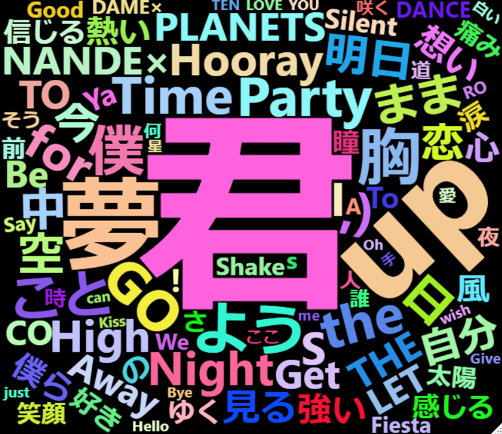
\includegraphics[width=\hsize]{fig/wc8.png}
	\caption{８人時代}
	\label{fig:wc8}
\end{figure}
\begin{figure}[tb]
	\centering
	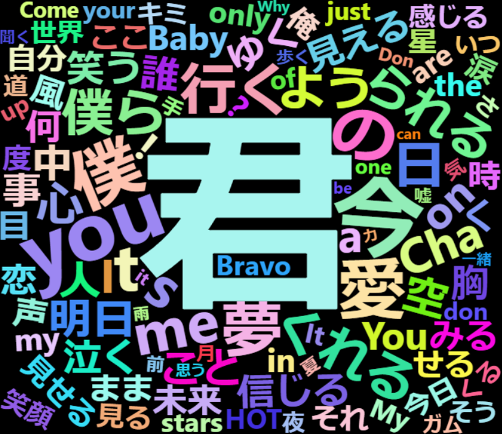
\includegraphics[width=\hsize]{fig/wc6.png}
	\caption{６人時代}
	\label{fig:wc6}
\end{figure}
\begin{figure}[tb]
	\centering
	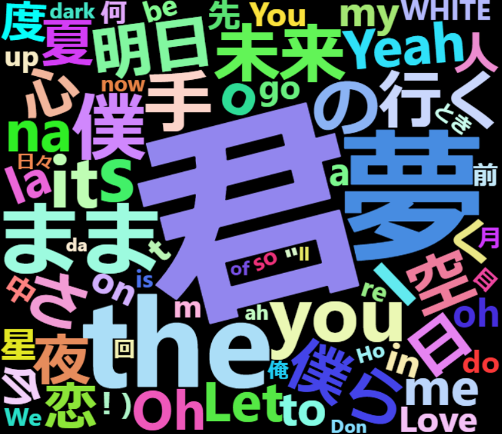
\includegraphics[width=\hsize]{fig/wc4.png}
	\caption{４人時代}
	\label{fig:wc4}
\end{figure}
\begin{figure}[tb]
	\centering
	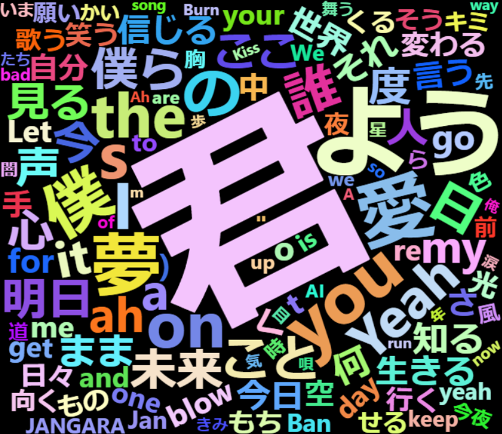
\includegraphics[width=\hsize]{fig/wc3.png}
	\caption{３人時代}
	\label{fig:wc3}
\end{figure}


それぞれの時代において活動年数が異なり，特に9人時代はNEWSニッポンとそのカップリング曲の計2曲しかないためデータとしての信頼性は低いといえる．
そのことを踏まえ，特徴的な単語の数の内訳に触れながら各時代の特徴を述べていく．

\subsubsection{9人時代}
「NEWS」「誰」「AWAY」の3つが目立っている．「NEWS」に関してはグループ名と同じなのだが，これはデビュー曲，NEWSニッポンの中でリフレインが繰り返されていたことが要因だと思われる．
旧ジャニーズ事務所からデビューしたグループの多くはデビュー曲で自身のグループ名が歌詞に取り入れられていることが多い．NEWS以外にも嵐の「A・RA・SHI(1999)\cite{ARASHI}」やHey!Say!JUMPの「Ultra Music Power(2007)\cite{JUMP}」，SexyZoneの「SexyZone(2011)\cite{SZ}」などが例に挙げられる．そのためこのワードクラウドはその影響が色濃く反映されているといえる．

\subsubsection{8人時代}
「君」が最も目立っている．この単語に関してはこれ以降の時代でも目立っているため全体を通して多用されていることがわかる．
この時代と他と比較すると「up」の多さを感じる．また「PLANETS」「NANDE×」「Hooray」「Time」「Party」などの英単語が目立っていると感じる．これらの英単語はどれも1～2曲（「Time」のみ4曲）のみで使われている．8人時代も9人時代と同じく，約3年間の活動で25曲しかない．そのため一曲のリフレインが多い区影響しているともいえる．

\subsubsection{6人時代}
「君」を除くと「今」「愛」「僕」が目立っていると感じた．しかし，6人時代は2007から2011年の約5年間の活動期間があり今回の調査対象は65曲ある．そのため特徴的な単語というよりはどの楽曲でも使用されるような汎用性の高い単語が表示さえている可能性が高い．

\subsubsection{4人時代}
「君」を除くと「夢」が目立っている．「夢」自体は8人時代からすべてのワードクラウドに入っているが4人時代が顕著に多い．4人時代は2012から2020の約9年間で今回調査対象は111曲ある．そのため6人時代よりも汎用性の高い単語が表示されている可能性が高い．しかし，その中でも「夢」の大きさは顕著でありこの時代の一つの特徴といえると考えた．

\subsubsection{3人時代}
「君」を除くと「僕」「夢」などが目立っている印象にあり比較的6人時代と似たような傾向にあると感じる．3人時代は2020から現在に至る約5年の活動期間で対象楽曲の数は63曲となっている．6人時代とほぼ同じ母集団の数であるためリフレインの数の影響などが似ており結果が似たものになったのではないかと考える．

全体的にポジティブな単語が多い傾向にあり「君」「夢」が特徴的といえるだろう．

%\subsection{上位20単語の傾向}
%KHcoderを使用して上位150単語を選出し，そのうち上位20単語を示している．この150単語に出る品詞は「代名詞」「名詞」「サ変名詞」「形容動詞」「固有名詞」「組織名」「人名」「地名」「ナイ形容」「副詞可能」「未知語」「タグ」「感動詞」「動詞」「形容詞」「副詞」「名詞B」「動詞B」「形容詞B」「副詞B」「名詞C」「否定助動詞」「形容詞（非自立）」としている．

%\figref{fig:top20kaisu}，\figref{fig:top20kyoku}に上位20単語の使用回数と使用楽曲数のグラフを示す．


%\begin{figure}[tb]
%	\centering
%	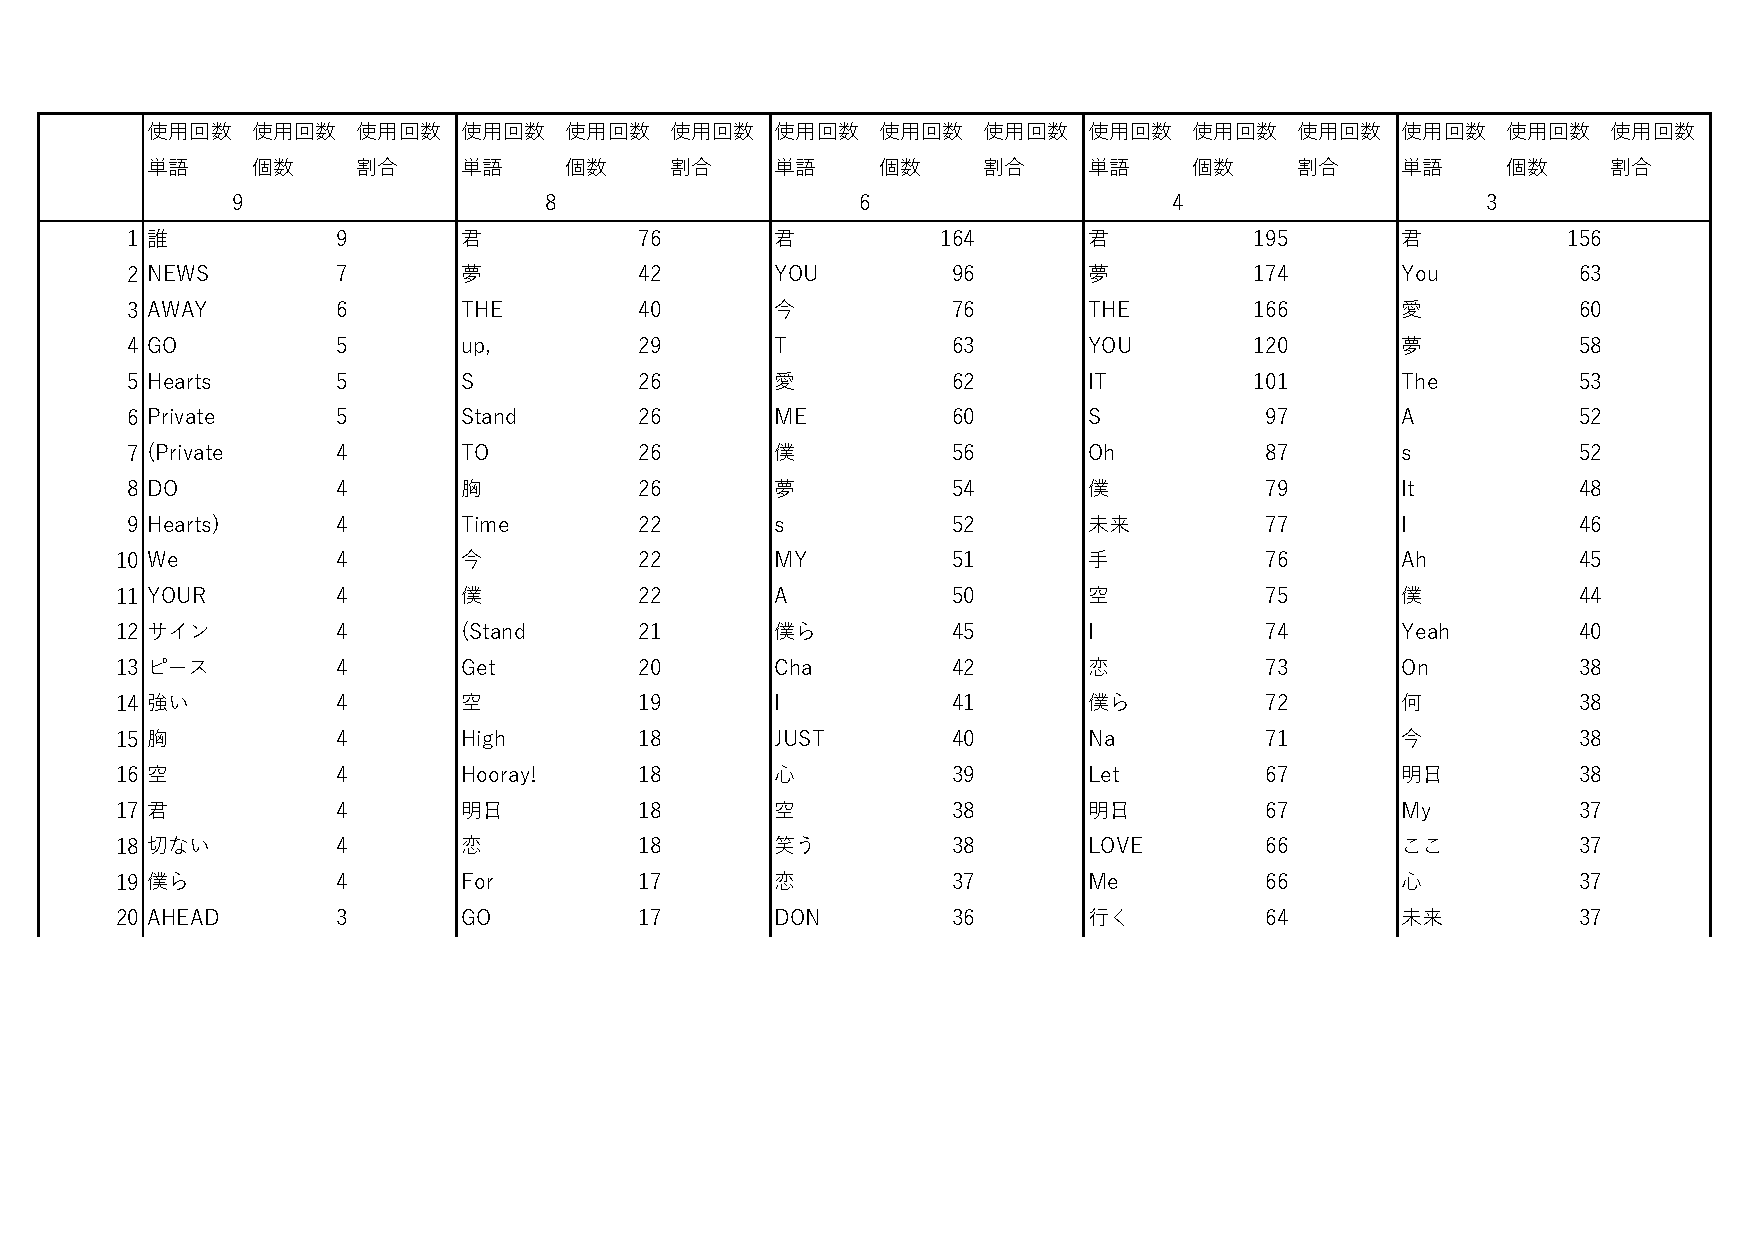
\includegraphics[width=\hsize]{fig/top20_kaisu.pdf}
%	\caption{各時代の上位20単語（使用回数）}
%	\label{fig:top20kaisu}
%\end{figure}
%\begin{figure}[tb]
%	\centering
%	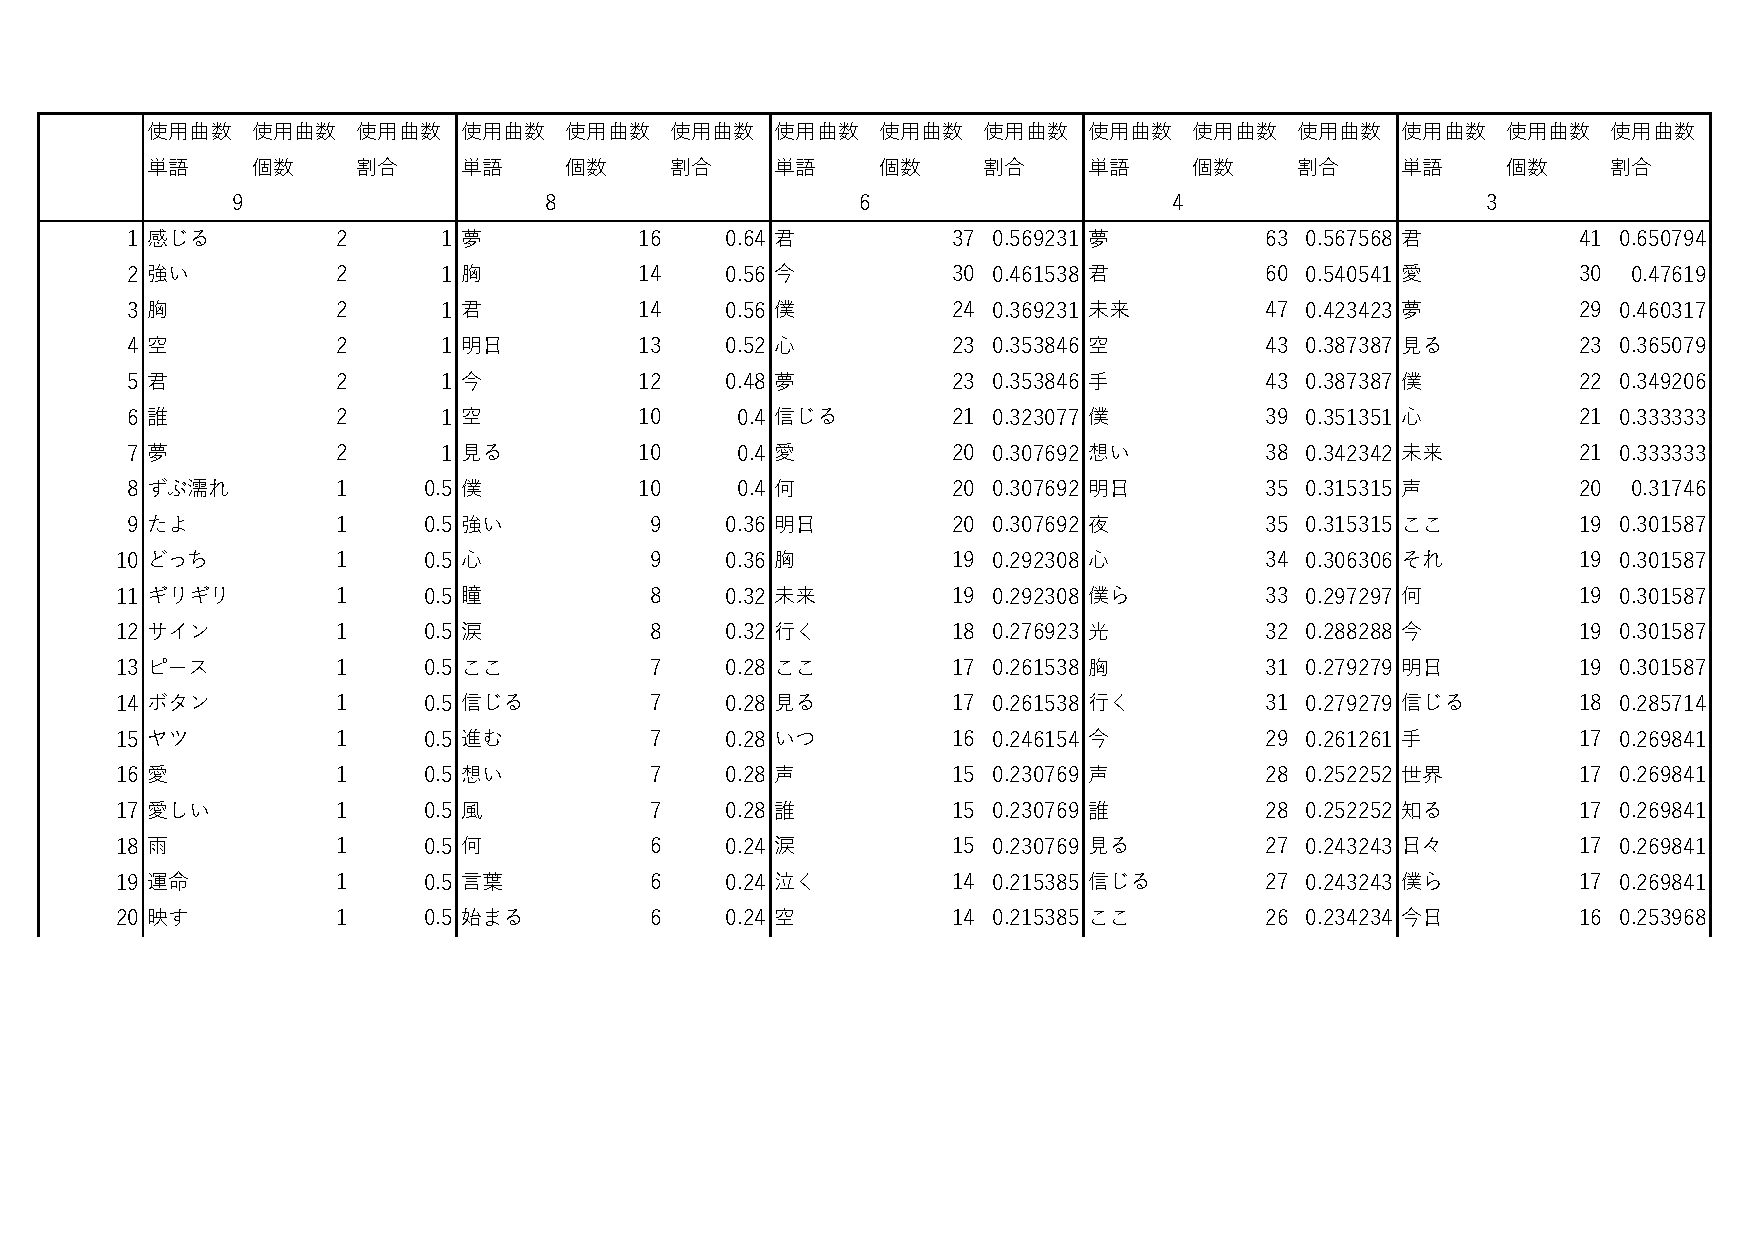
\includegraphics[width=\hsize]{fig/top20_kyokusu.pdf}
%	\caption{各時代の上位20単語（使用曲数）}
%	\label{fig:top20kyoku}
%\end{figure}




%ワードクラウドで確認した通り，9人時代以外は「君」が最も多く出ていることがわかる．もう一つ特徴と感じた「夢」だが，こちらも各時代で上位にいることからNEWS全体を通した特徴といえるだろう．

\subsection{品詞単位のネガポジ判定}
名詞，形容詞，動詞の3つに視点を当てRを使ったネガポジ判定を行った．ネガポジ判定とは感情分析の一種であり，文章に含まれる「嬉しい」や「悲しい」という感情表現に関する単語を抽出して解析を行う手法である．今回は日本語評価極性辞書（用言編）と日本語評価極性辞書（名詞編）\cite{ngpj}を使用した．

それぞれの人数時代ごとにテキストデータを用意し，形態素解析を行ったうえで辞書と照らし合わせる形をとった．

名詞はｐがポジティブ，nがネガティブ，eがニュートラルと分類されている．

形容詞，動詞はネガ（経験），ネガ（評価），ポジ（経験），ポジ（評価）の四つに分類している．

今回の比較では未分類，Noneとされている単語も多くあることが課題となった．


\begin{figure}[tb]
	\centering
	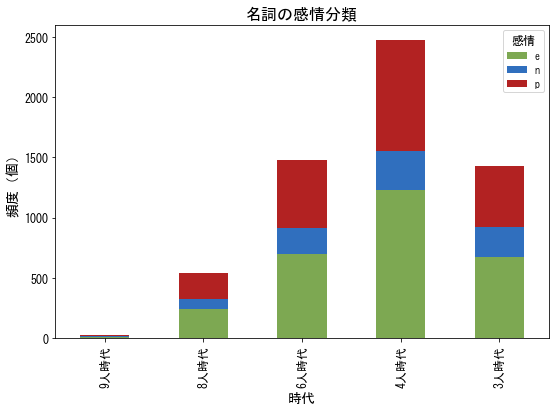
\includegraphics[width=\hsize]{fig/ngpj_meishi.png}
	\caption{ネガポジ判定（名詞）}
	\label{fig:ngpj_meishi}
\end{figure}

\begin{figure}[tb]
	\centering
	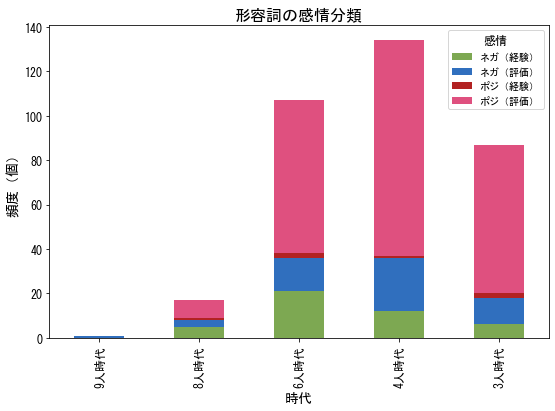
\includegraphics[width=\hsize]{fig/ngpj_keiyoushi.png}
	\caption{ネガポジ判定（形容詞）}
	\label{fig:ngpj_keiyoushi}
\end{figure}
\begin{figure}[tb]
	\centering
	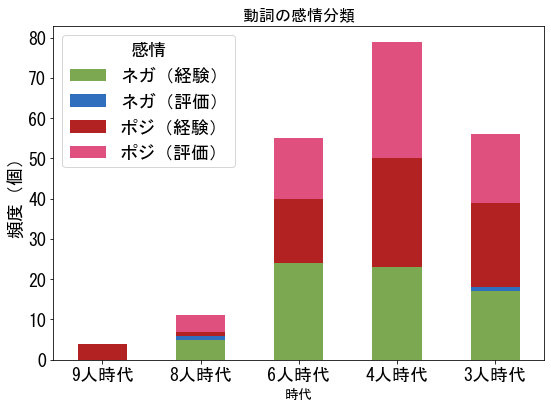
\includegraphics[width=\hsize]{fig/ngpj_doushi.png}
	\caption{ネガポジ判定（動詞）}
	\label{fig:ngpj_doushi}
\end{figure}

9人時代は2曲しかないため参考程度にとどめるべきだろう．

名詞は全体的に一目見た各感情の比率は同じように見える．つまりネガティブ，ポジティブ，ニュートラルの割合が人数によって変わったわけではないと読み取れる．

形容詞は人数編成が変わるたびにポジティブの割合が増える傾向が読み取れる．

動詞は4人以降，ポジティブの割合が増えたと読み取れた．

いずれにせよ，Noneの割合が著しく高いことが課題となった．
\begin{figure}[h]
	\centering
	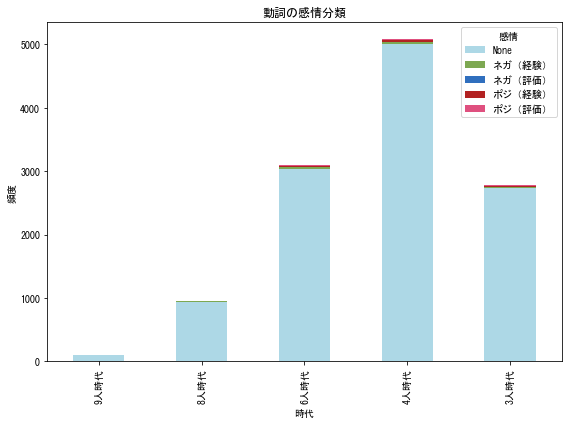
\includegraphics[width=\hsize]{fig/ngpj_doushi_none.png}
	\caption{ネガポジ判定（動詞）Noneを含む}
	\label{fig:ngpj_doushi_none}
\end{figure}

\figref{fig:ngpj_doushi_none}はNoneを含めた動詞の結果だが，特に活用の多い動詞はNoneの割合が著しく多い．
このようなことからネガポジ判定については分析方法について精査の余地があると考える．

%\begin{figure}[tb]
%\centering
%	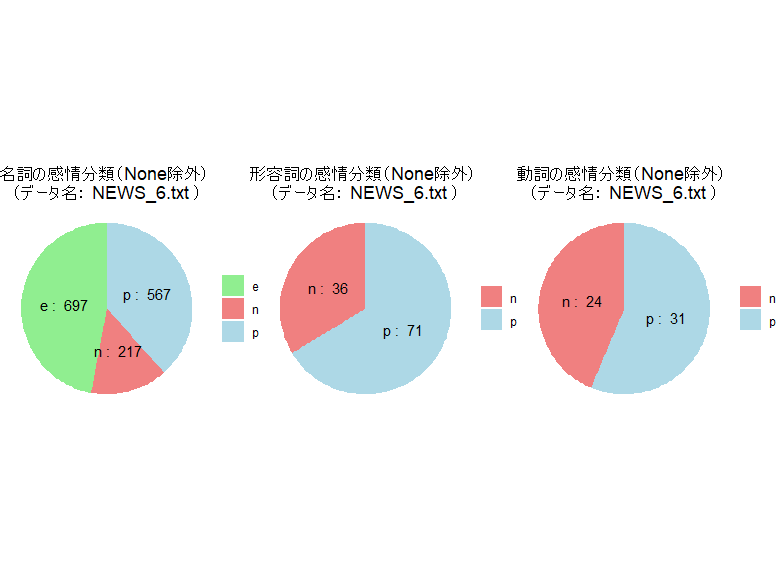
\includegraphics[width=\hsize]{fig/np6.png}
%	\caption{ネガポジ判定（６人時代）}
%	\label{fig:np6}
%\end{figure}
%\begin{figure}[tb]
%%	\centering
%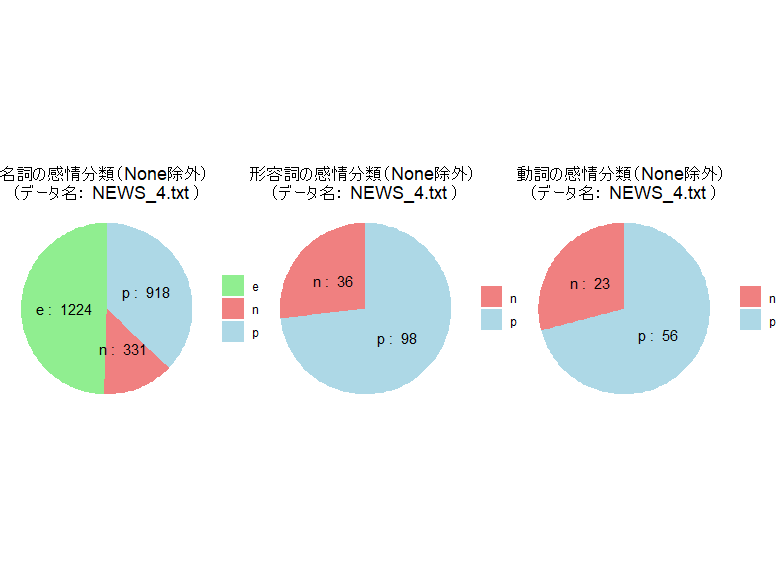
\includegraphics[width=\hsize]{fig/np4.png}
%\caption{ネガポジ判定（４人時代）}
%\label{fig:np4}
%\end{figure}





\subsection{品詞別の使用頻度推移}\label{sec:hinshi-suii}
ここでは使用単語数と使用楽曲数の2種類の表をそれぞれ出している．これはリフレインの影響を考慮したものになる．例えば「チャンカパーナ」という単語は18回使用されているがすべてチャンカパーナ(2012)のみで使用された回数になる．一曲のみでしか使われていないにもかかわらずリフレインによって上位に来る可能性がある単語があるのだ．もちろん，リフレインをすること自体に意味がある場合もある．そのため今回は使用楽曲数を使用単語数に分けて比較することにした．また時系列別にグラフを出力する際，9人時代が2曲しかなくサンプル数が少ないため今回は省いている．

%品詞表の中身はすべて付録にある．ここではその中で筆者主観の各品詞の特徴的な単語について人数時代別に比較ぐラグを表示する．
%みたいな流れにしたい，付録どうしようか

% ----------- 代名詞 -------------------------


\subsubsection{代名詞}
\begin{figure}[tb]
	\centering
	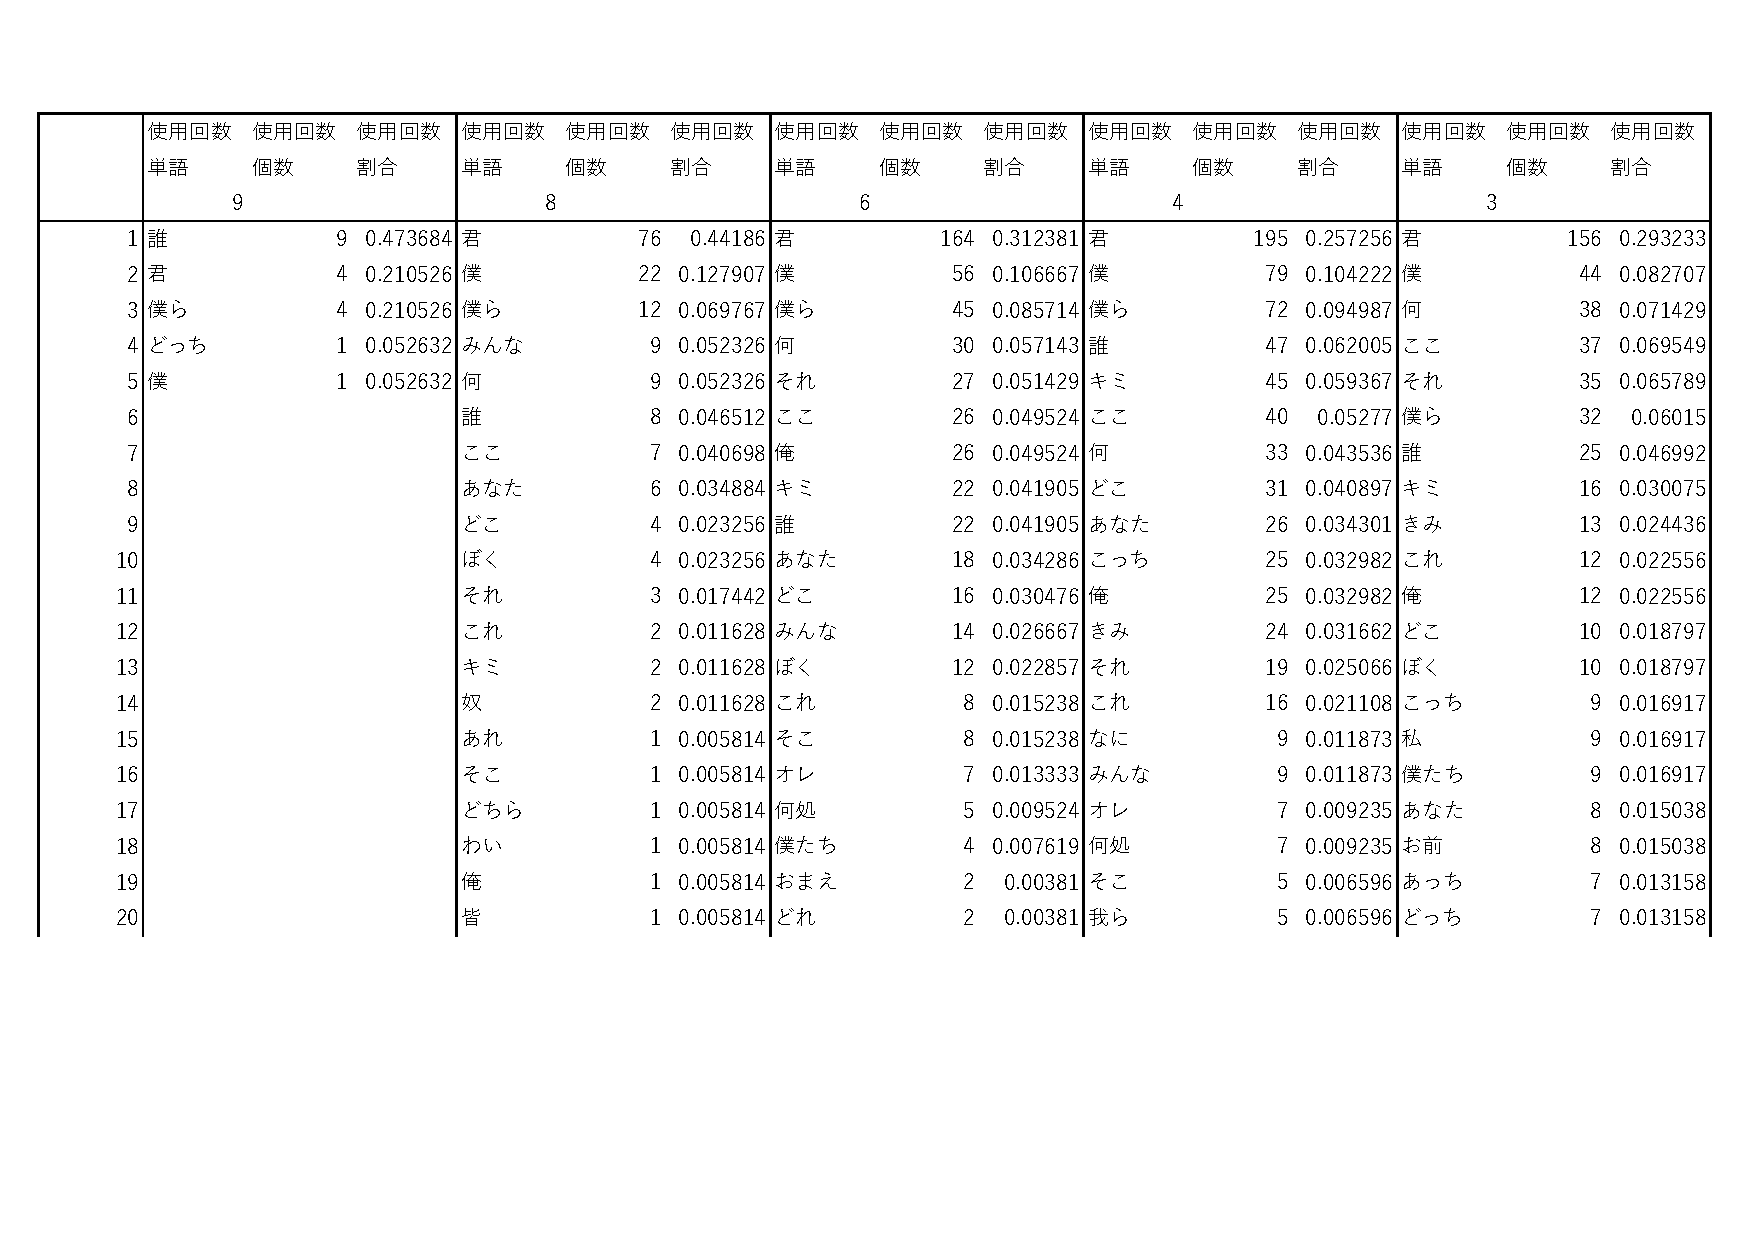
\includegraphics[width=\columnwidth]{fig/w-daimei-kaisu.pdf}\vspace{12pt}
	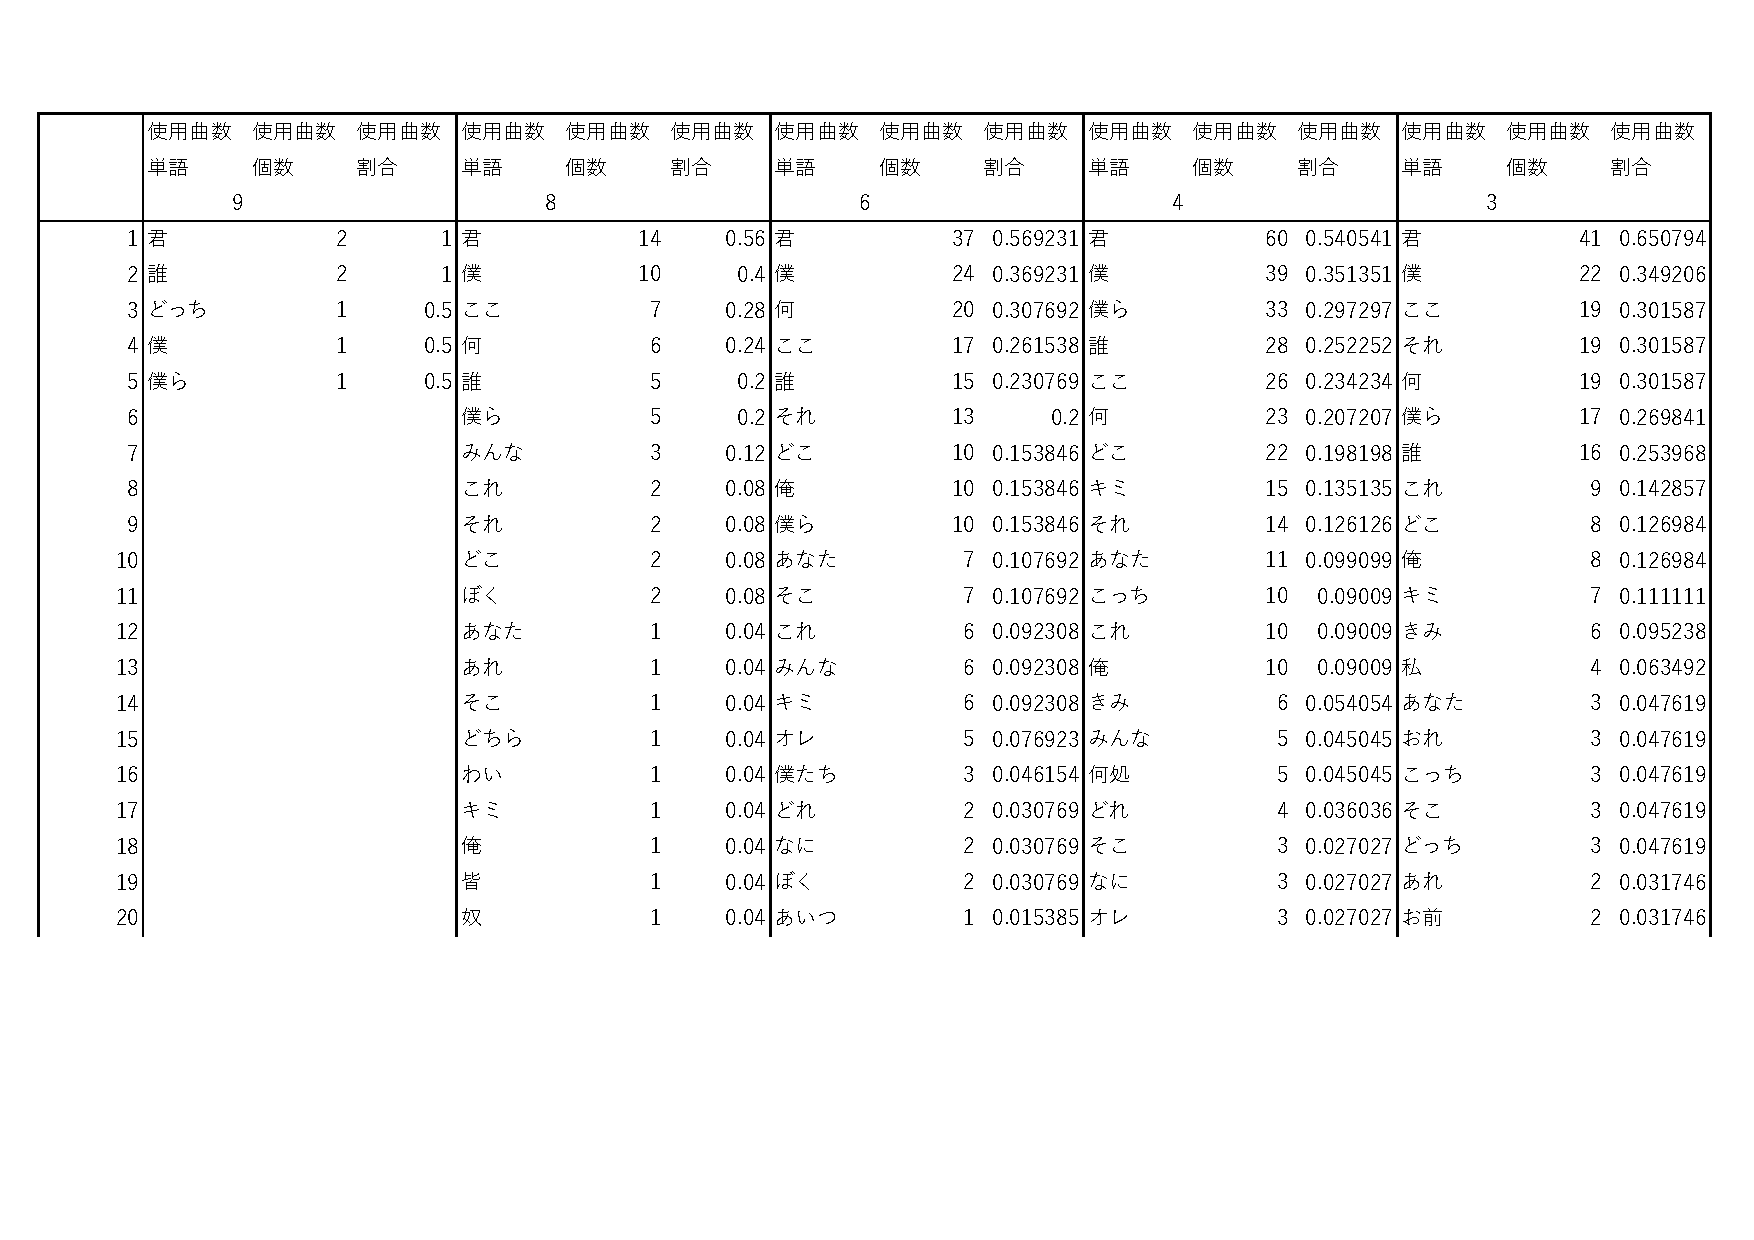
\includegraphics[width=\columnwidth]{fig/w-daimei-kyokusu.pdf}
	\caption{代名詞の使用回数（上），使用曲数（下）}
	\label{fig:daimei}
\end{figure}

\figref{fig:daimei}に代名詞の使用回数，使用楽曲の上位20個を表示した表を示す．

どの人数時代でも使用回数，使用楽曲数ともに「君」が最も使用されていたことがわかる．

\figref{fig:kimi}より，「君」の使用回数ではどの人数時代でも全体と比較して3割程度，もしくはそれ以上の使用回数があることが確認できる．
また使用曲数においてもどの人数時代でも5割以上の楽曲で「君」を使用していることがわかる．

\begin{figure}[tb]
	\centering
	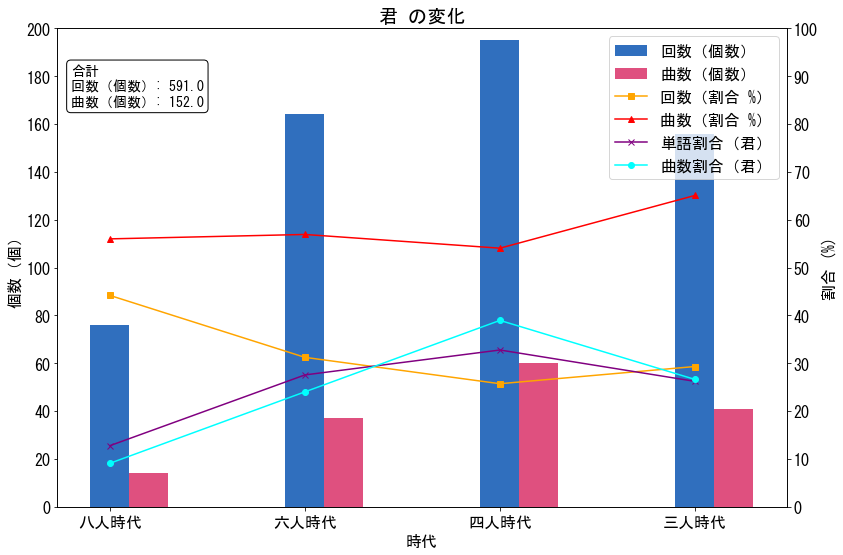
\includegraphics[width=\hsize]{fig/kimi.png}
	\caption{「君」の比較グラフ}
	\label{fig:kimi}
\end{figure}


% ----------- 動詞 -------------------------
\subsubsection{動詞}
\figref{fig:verb}に動詞の使用回数，使用楽曲の上位20個を表示した表を示す．

\begin{figure}[tb]
	\centering
	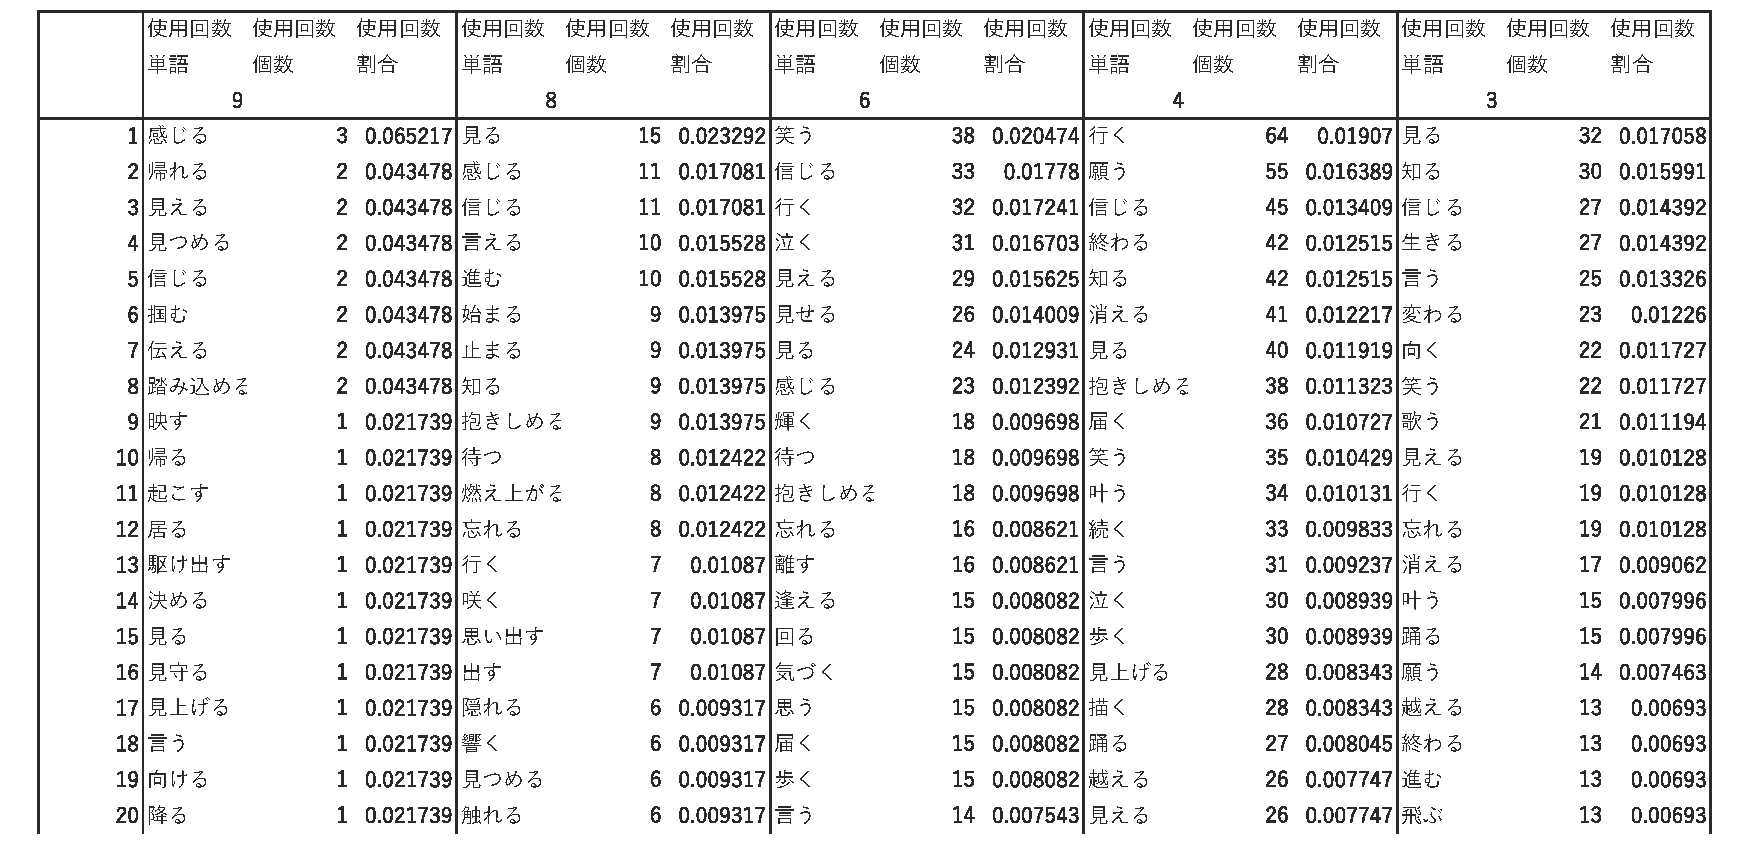
\includegraphics[width=\columnwidth]{fig/w-verb-kaisu.pdf}\vspace{12pt}
	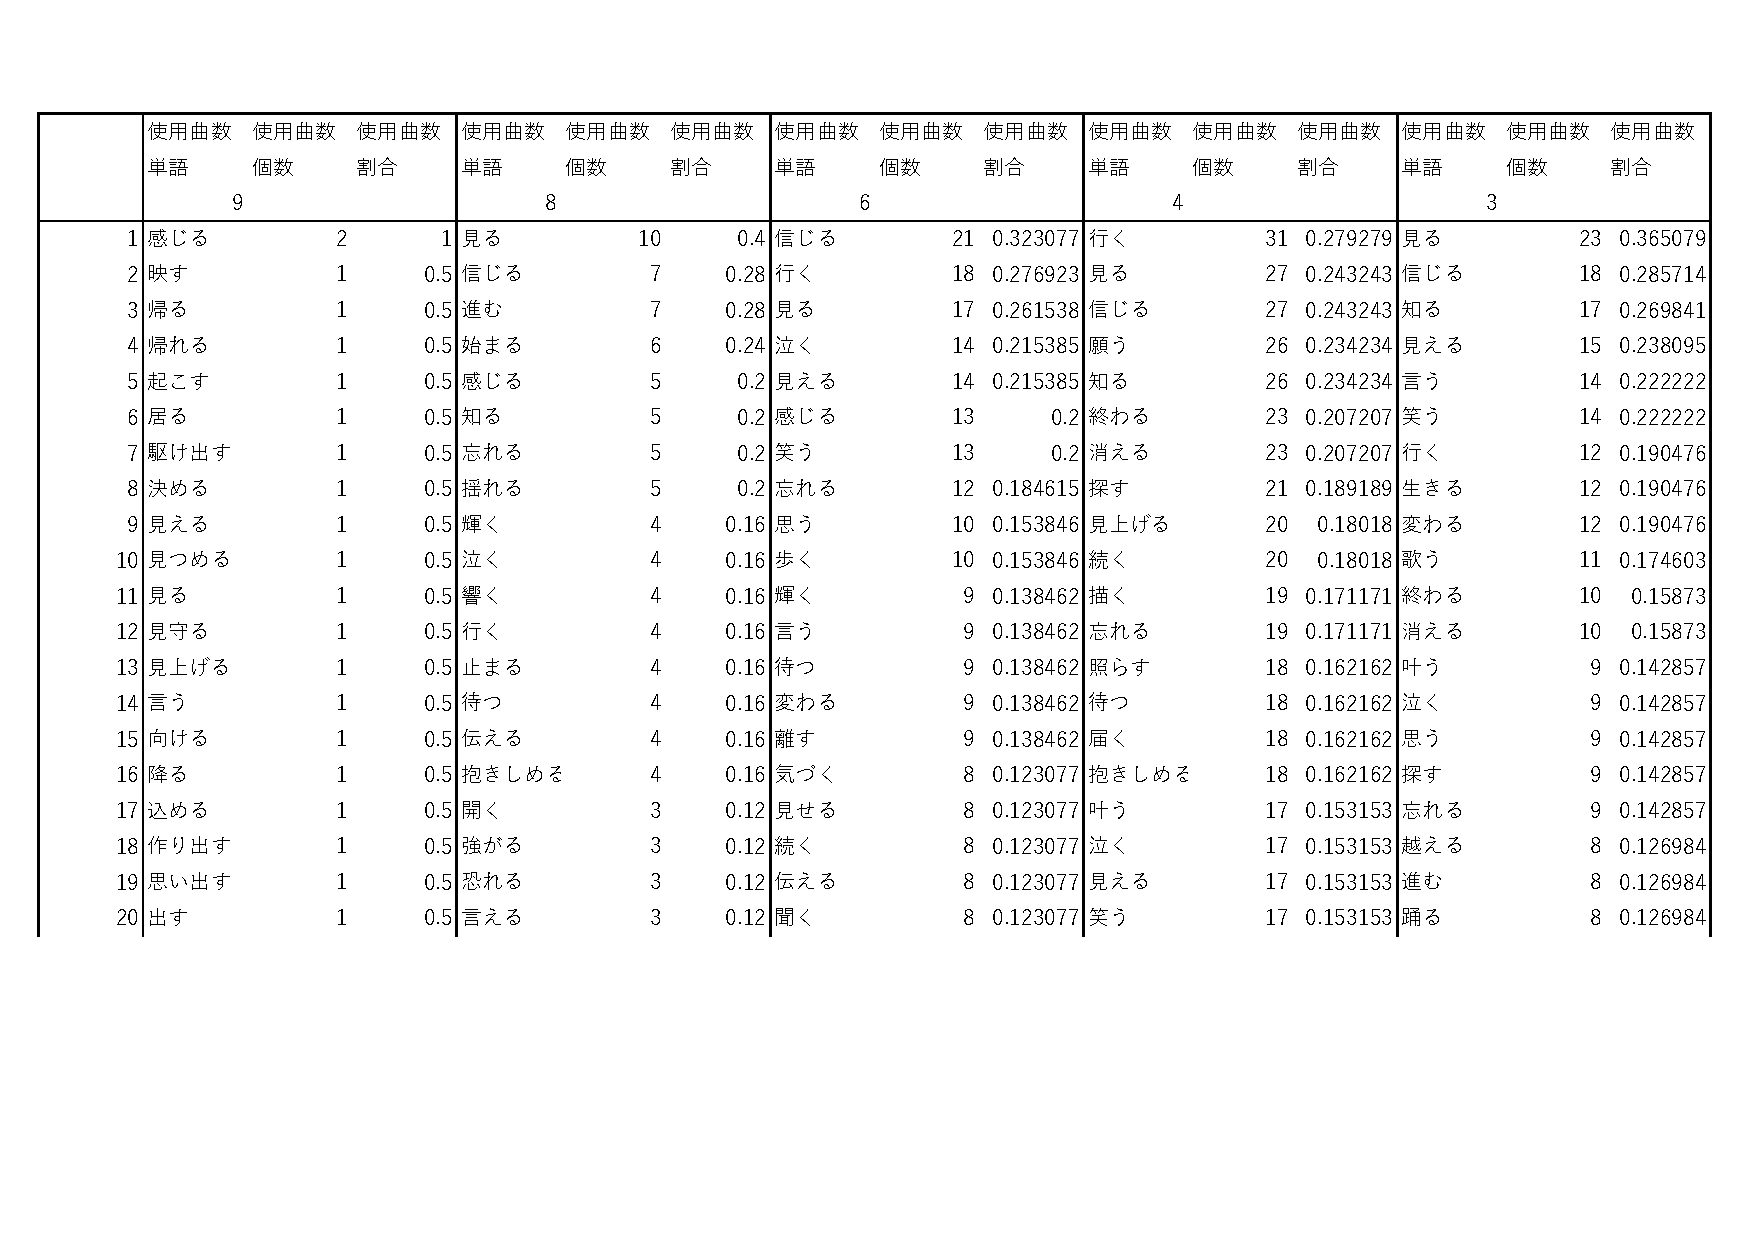
\includegraphics[width=\columnwidth]{fig/w-verb-kyokusu.pdf}
	\caption{動詞の使用回数（上），使用曲数（下）}
	\label{fig:verb}
\end{figure}

使用回数と使用曲数で上位に違いがある．「信じる」が両者ともに上位3以内にいる．
6人時代と4人時代に絞って比較すると「願う」が上位にあり6人時代には上位になかった．
グラフで確認するとその違いは明らかである．




\begin{figure}[tb]
	\centering
	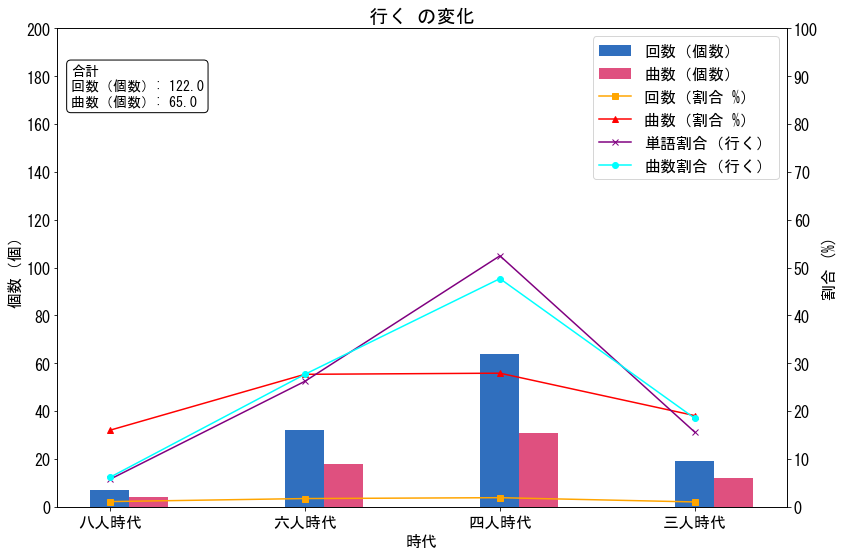
\includegraphics[width=\hsize]{fig/verb-iku.png}
	\caption{「行く」の比較グラフ}
	\label{fig:iku}
	%\end{figure}
	%\begin{figure}[tb]
	\centering
	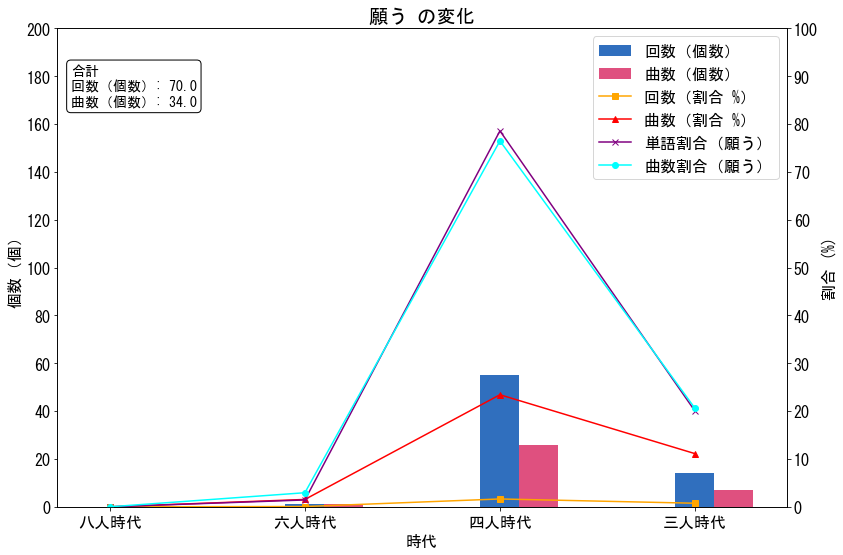
\includegraphics[width=\hsize]{fig/verb-negau.png}
	\caption{「願う」の比較グラフ}
	\label{fig:negau}
	%\end{figure}
	%\begin{figure}[tb]
	\centering
	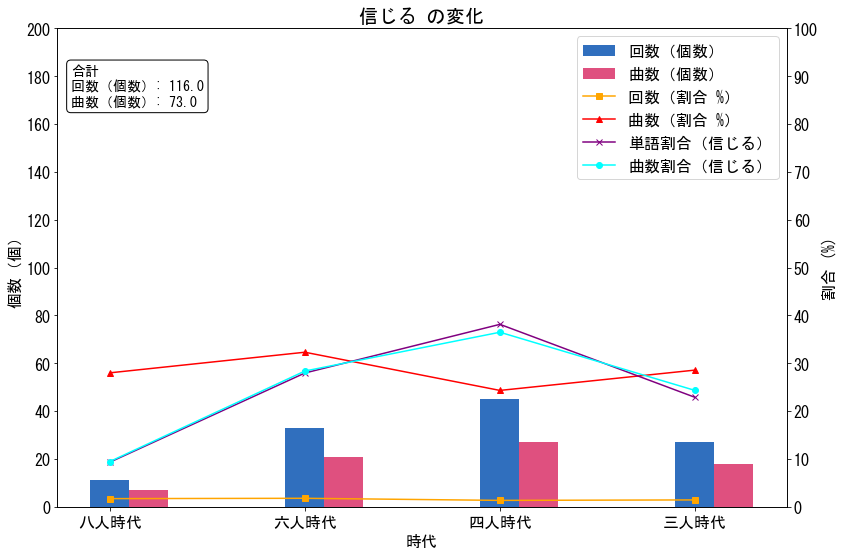
\includegraphics[width=\hsize]{fig/verb-shinjiru.png}
	\caption{「信じる」の比較グラフ}
	\label{fig:shinjiru}
\end{figure}


\figref{fig:iku}，\figref{fig:negau}，\figref{fig:shinjiru}を比較したとき，4人時代の楽曲が最も多く，六人時代や三人時代と比較して倍の楽曲数があるため必然的に4人が多くなる傾向にあるのだが，「願う」に関してはそれが突出していることがわかる．

\subsubsection{形容詞}
\figref{fig:keiyo}に形容詞の使用回数，使用楽曲の上位20個を表示した表を示す．

\begin{figure}[tb]
	\centering
	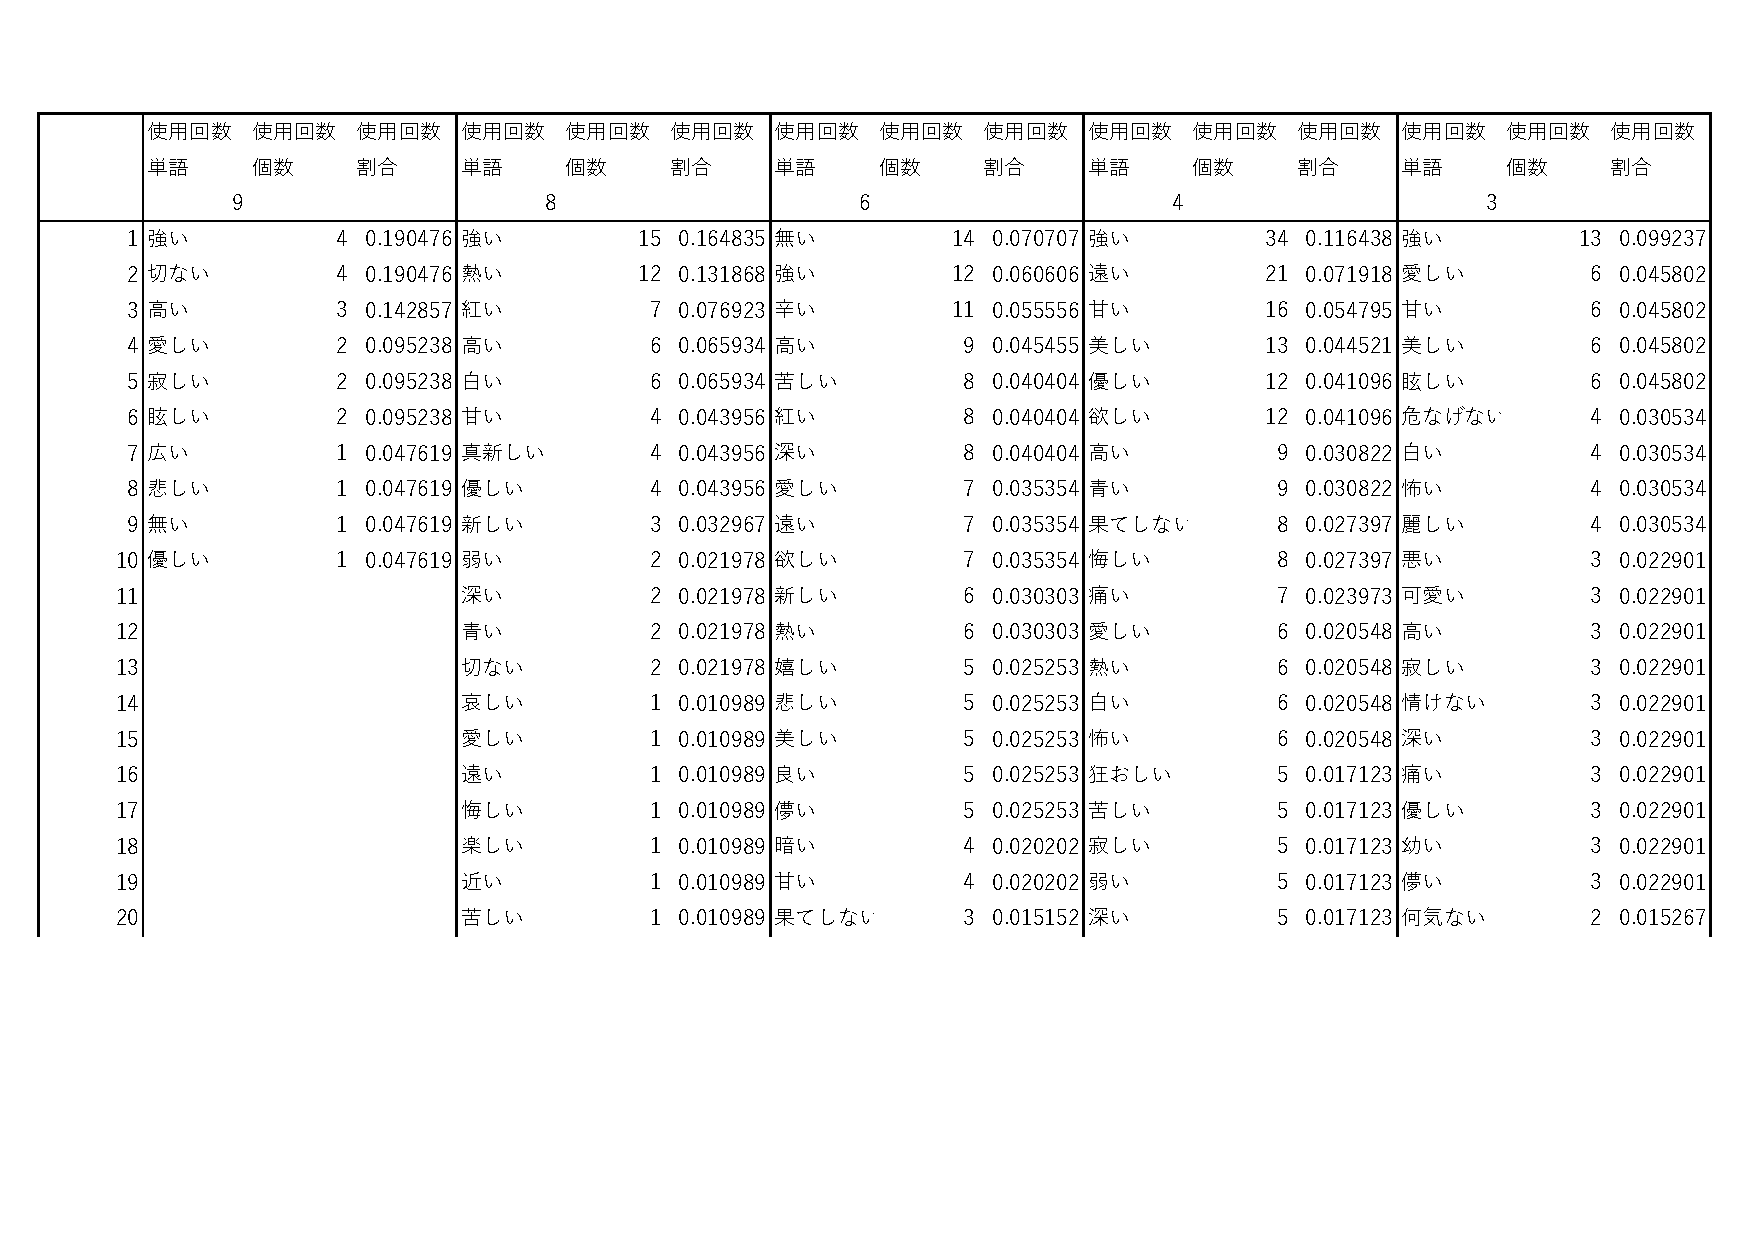
\includegraphics[width=\columnwidth]{fig/w-keiyo-kaisu.pdf}
	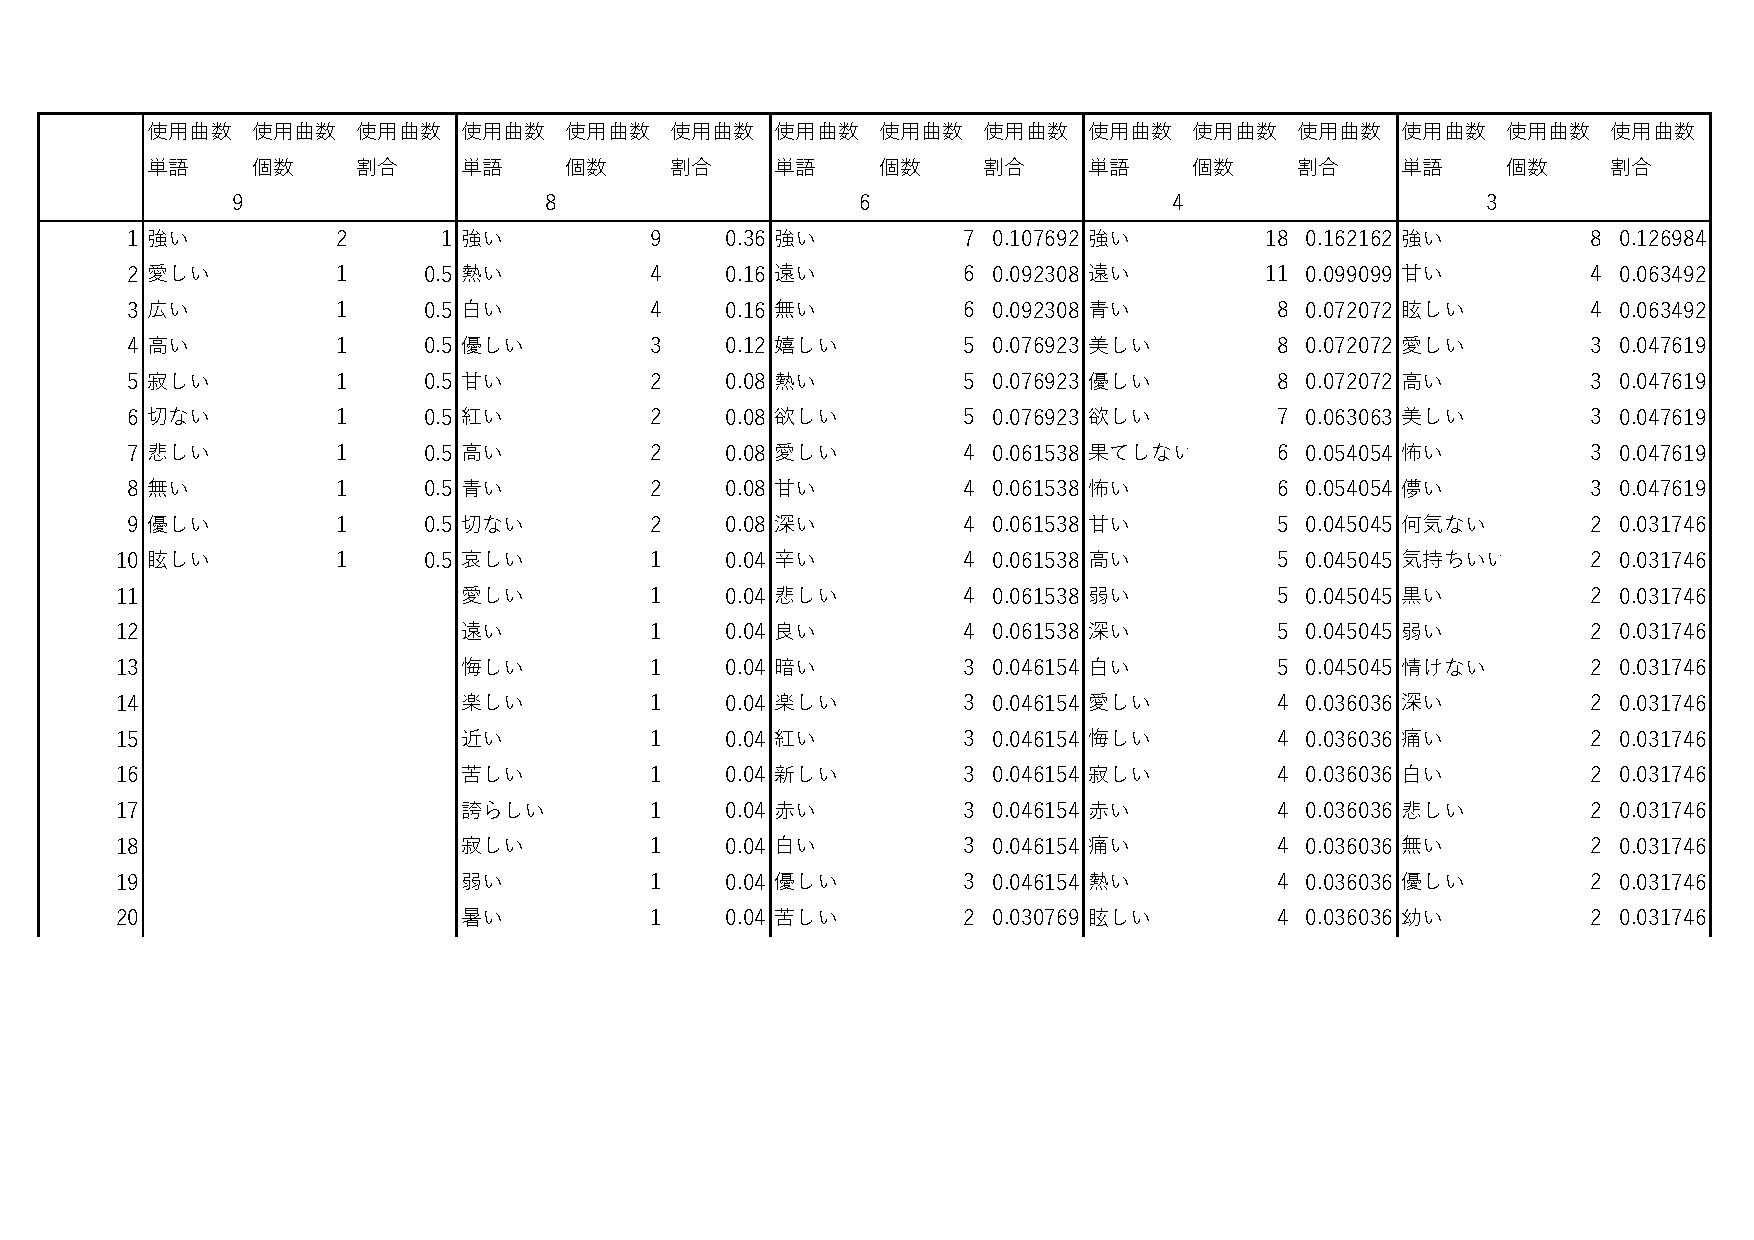
\includegraphics[width=\columnwidth]{fig/w-keiyo-kyokusu.pdf}
	\caption{形容詞の使用回数（上），使用曲数（下）}
	\label{fig:keiyo}
\end{figure}


6人時代の使用回数を除くすべてで最も多いのが「強い」であることがわかる\figref{fig:keiyo}．
また6人時代の使用回数で最も多い「無い」が他ではあまり出現していないことが気になった．
この2単語についてグラフで表示する（\figref{fig:tsuyoi}，\figref{fig:nai}）．

\begin{figure}[tb]
	\centering
	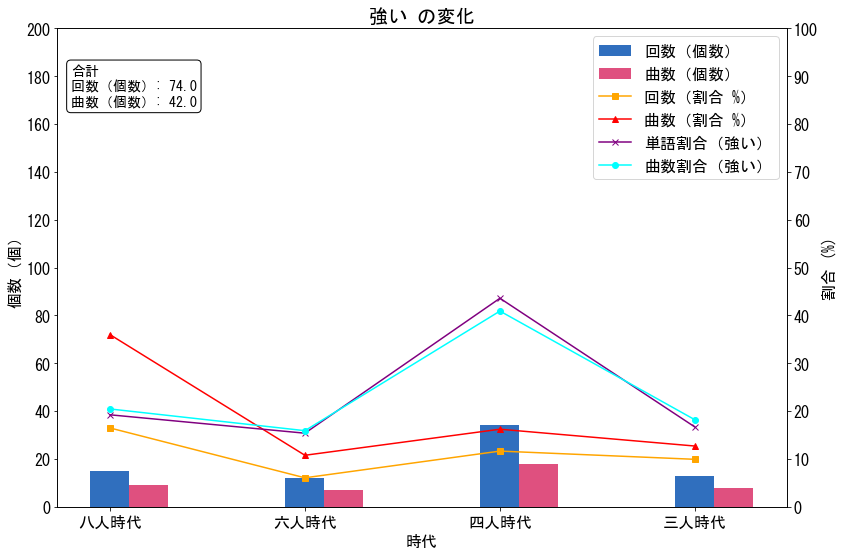
\includegraphics[width=\hsize]{fig/keiyo-tsuyoi.png}
	\caption{「強い」の比較グラフ}
	\label{fig:tsuyoi}
	%\end{figure}

	%\begin{figure}[tb]
	\centering
	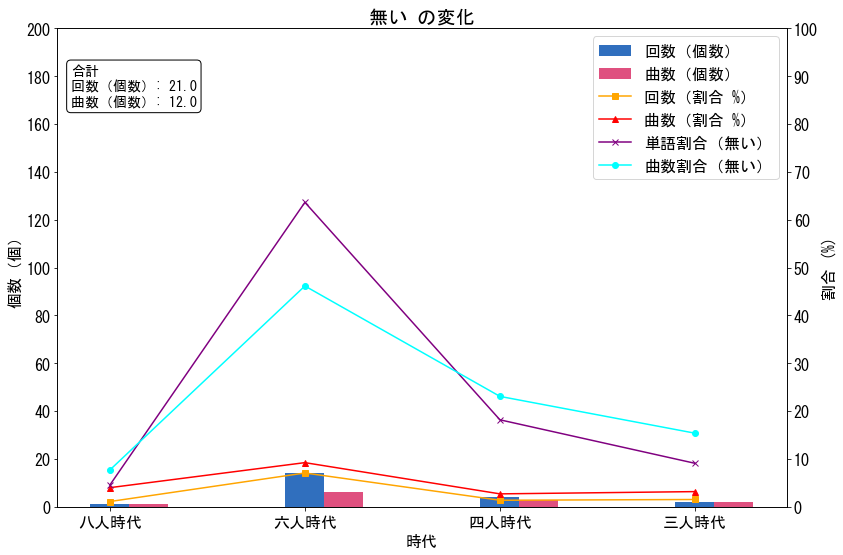
\includegraphics[width=\hsize]{fig/keiyo-nai.png}
	\caption{「無い」の比較グラフ}
	\label{fig:nai}
\end{figure}

動詞で述べた通り，楽曲数などが考慮されるため4人が突出するグラフが比較的多い．その中で六人時代が最も多くなっている「無い」はこの時代の特徴とみられる．


\subsubsection{副詞}
\figref{fig:fuku}に副詞の使用回数，使用楽曲の上位20個を表示した表を示す．

\begin{figure}[tb]
	\centering
	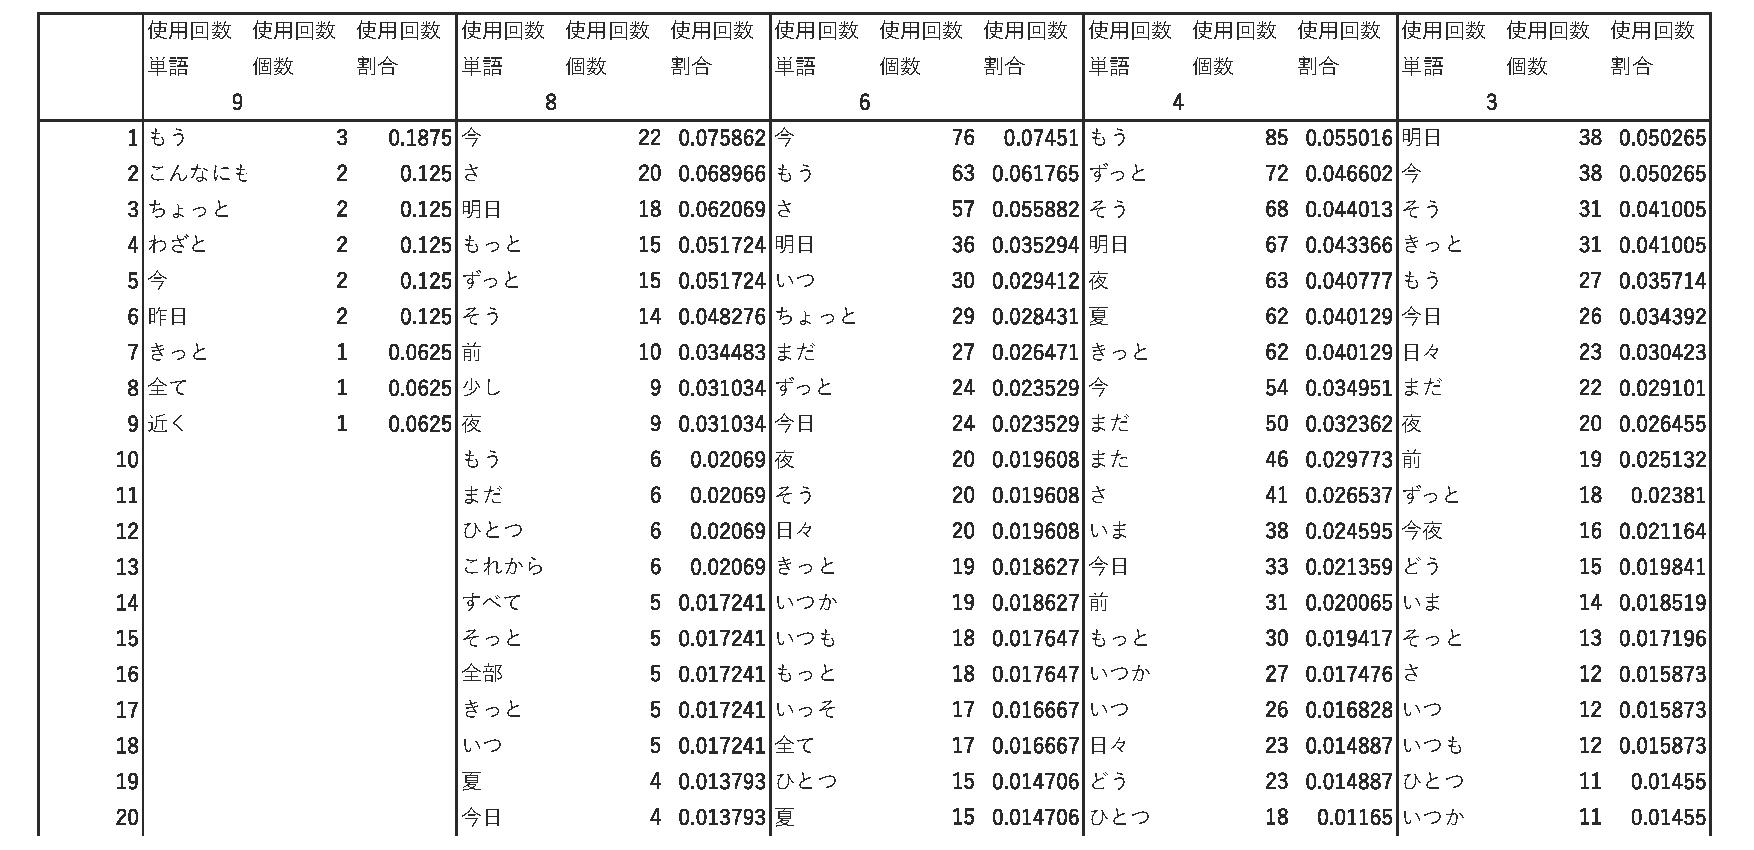
\includegraphics[width=\columnwidth]{fig/w-fuku-kaisu.pdf}
	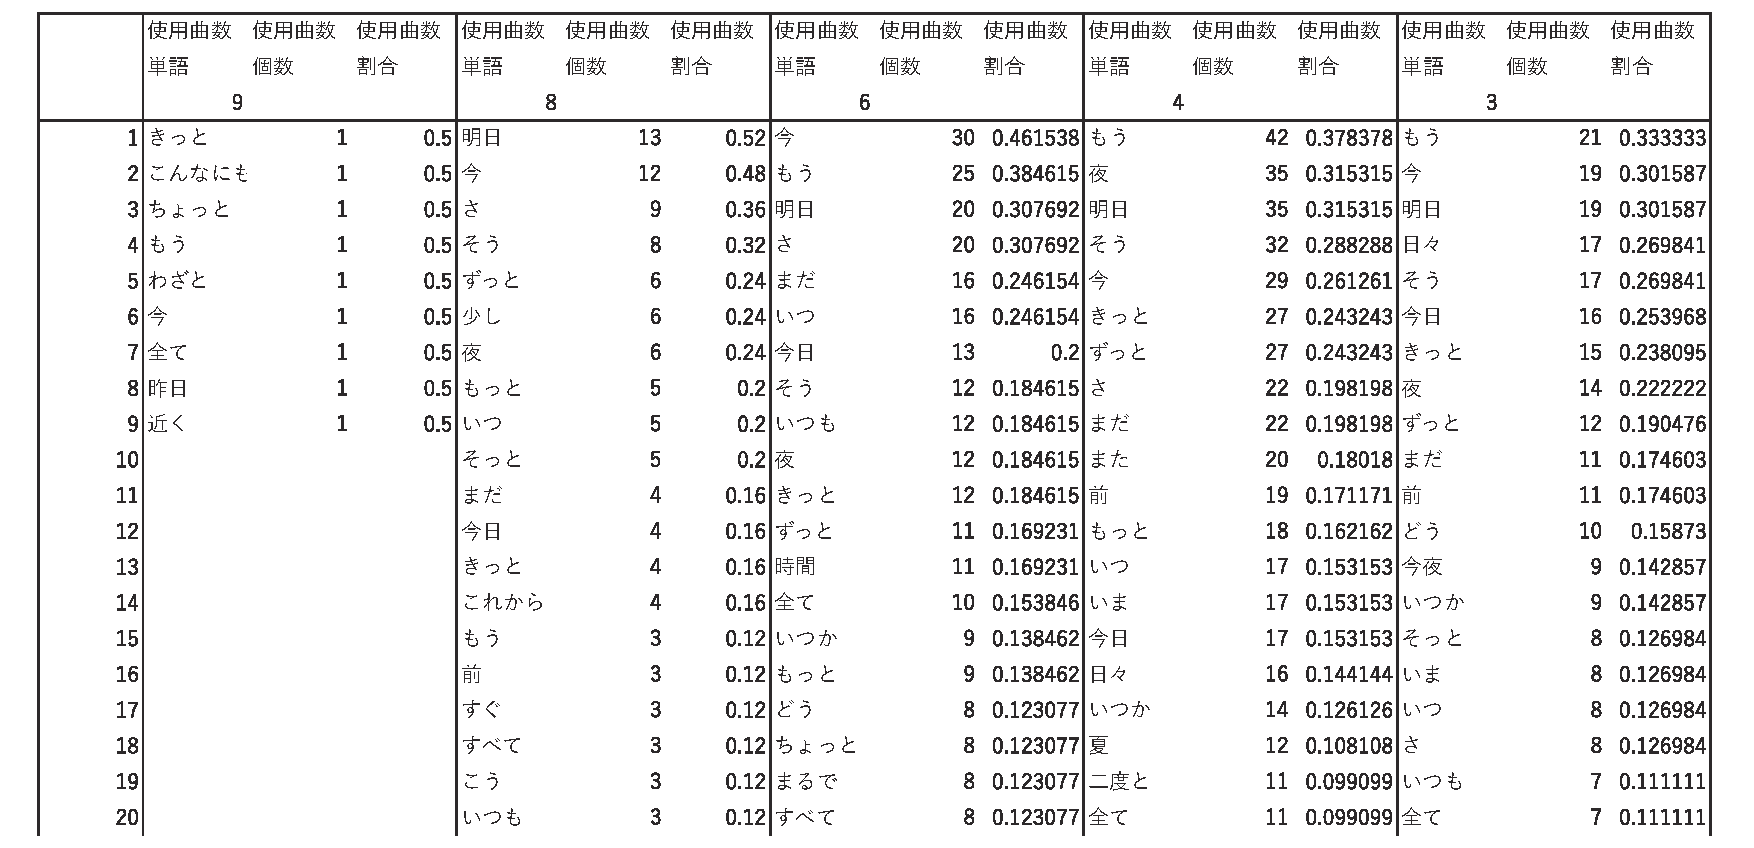
\includegraphics[width=\columnwidth]{fig/w-fuku-kyokusu.pdf}
	\caption{副詞の使用回数（上），使用曲数（下）}
	\label{fig:fuku}
\end{figure}

季節を表す春夏秋冬のうち「夏」だけが出現することが多いのが気になりグラフで比較した（\figref{fig:natsu}）．
その結果「夏」はどの時代でも一定の数の出現が確認できた．

\begin{figure}[tb]
	\centering
	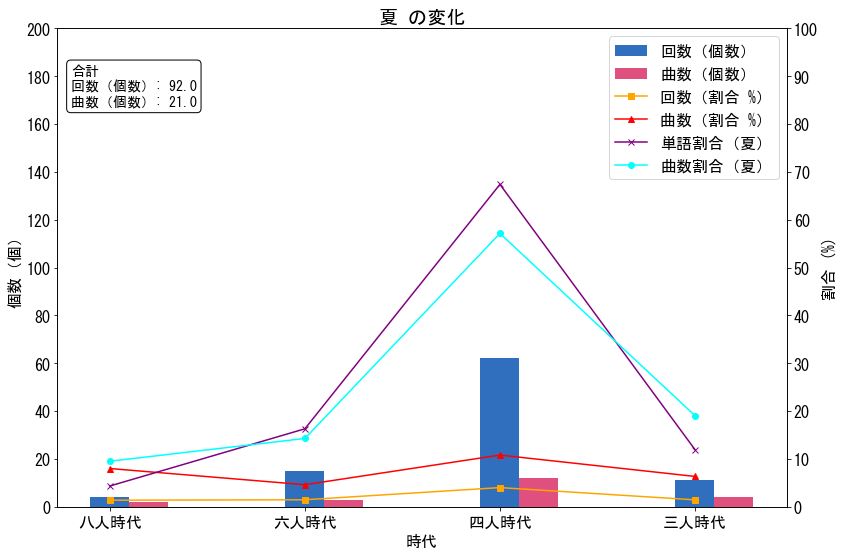
\includegraphics[width=\hsize]{fig/fuku-natsu.png}
	\caption{「夏」の比較グラフ}
	\label{fig:natsu}
\end{figure}


「今」「明日」など現在を基準にすると未来を表す言葉が多く，4人の特徴では「ずっと」が多いのが特徴的であると考えた．

\figref{fig:ima}，\figref{fig:asu}，\figref{fig:zutto}で比較する．

\begin{figure}[tb]
	\centering
	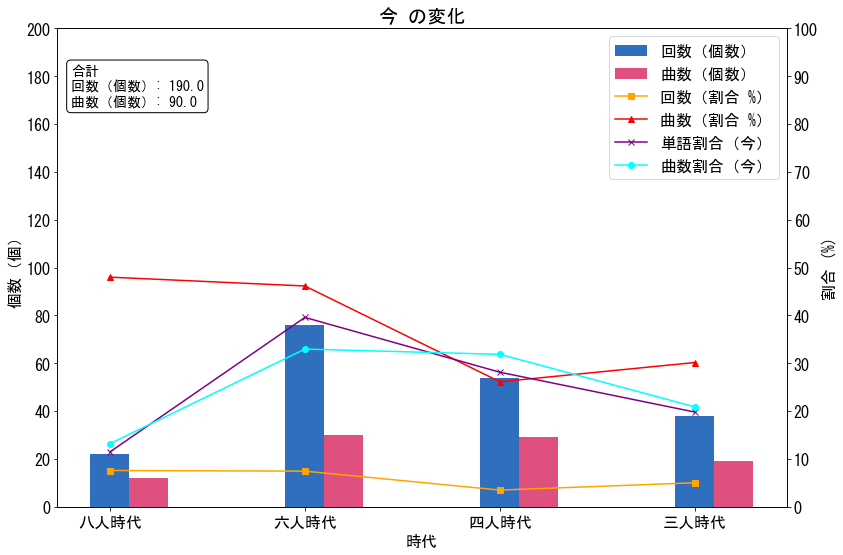
\includegraphics[width=\hsize]{fig/fuku-ima.png}
	\caption{「今」の比較グラフ}
	\label{fig:ima}
	%\end{figure}
	%\begin{figure}[tb]
	\centering
	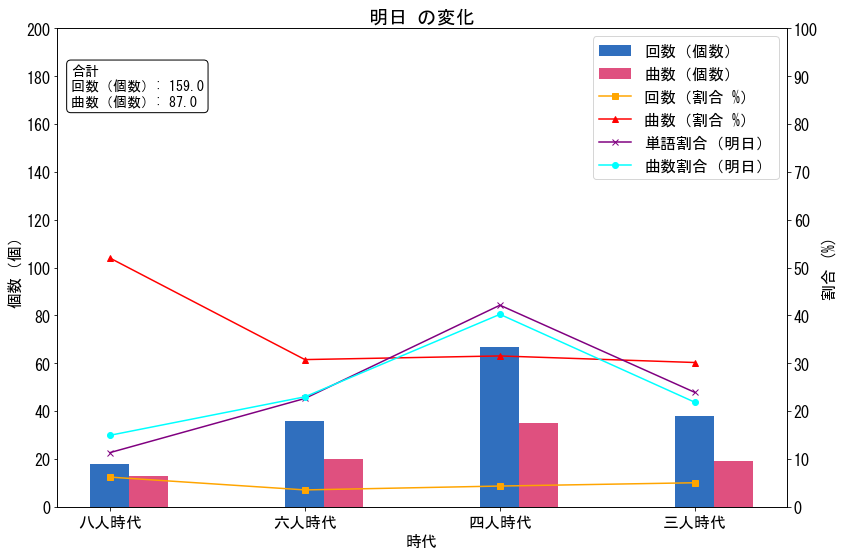
\includegraphics[width=\hsize]{fig/fuku-asu.png}
	\caption{「明日」の比較グラフ}
	\label{fig:asu}
	%\end{figure}
	%\begin{figure}[tb]
	\centering
	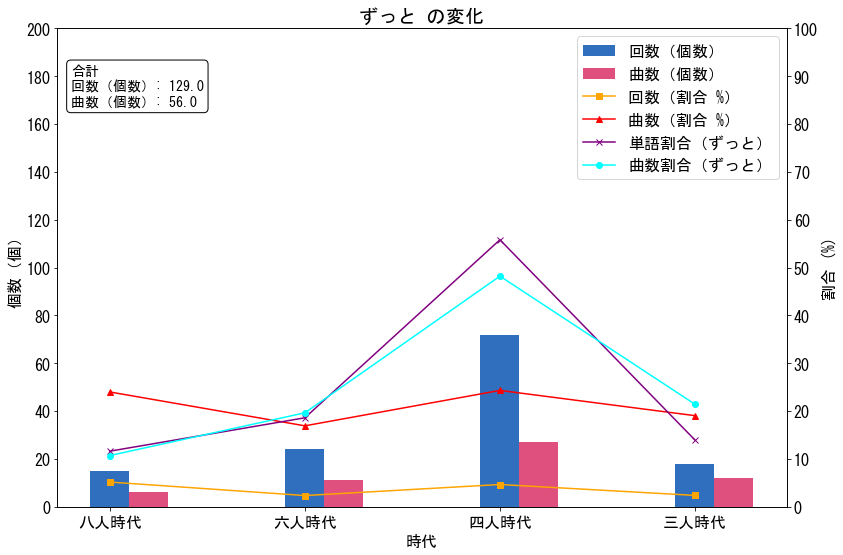
\includegraphics[width=\hsize]{fig/fuku-zutto.png}
	\caption{「ずっと」の比較グラフ}
	\label{fig:zutto}
\end{figure}

6人時代は「今」を歌うことが多かったことに対して，4人時代は「明日」を歌うことが多かったと見て取れる．
また「ずっと」とこれから先を指す単語も特徴的だと考えた．

\subsubsection{名詞}
\figref{fig:meishi}に名詞の使用回数，使用楽曲の上位20個を表示した表を示す．


\begin{figure}[tb]
	\centering
	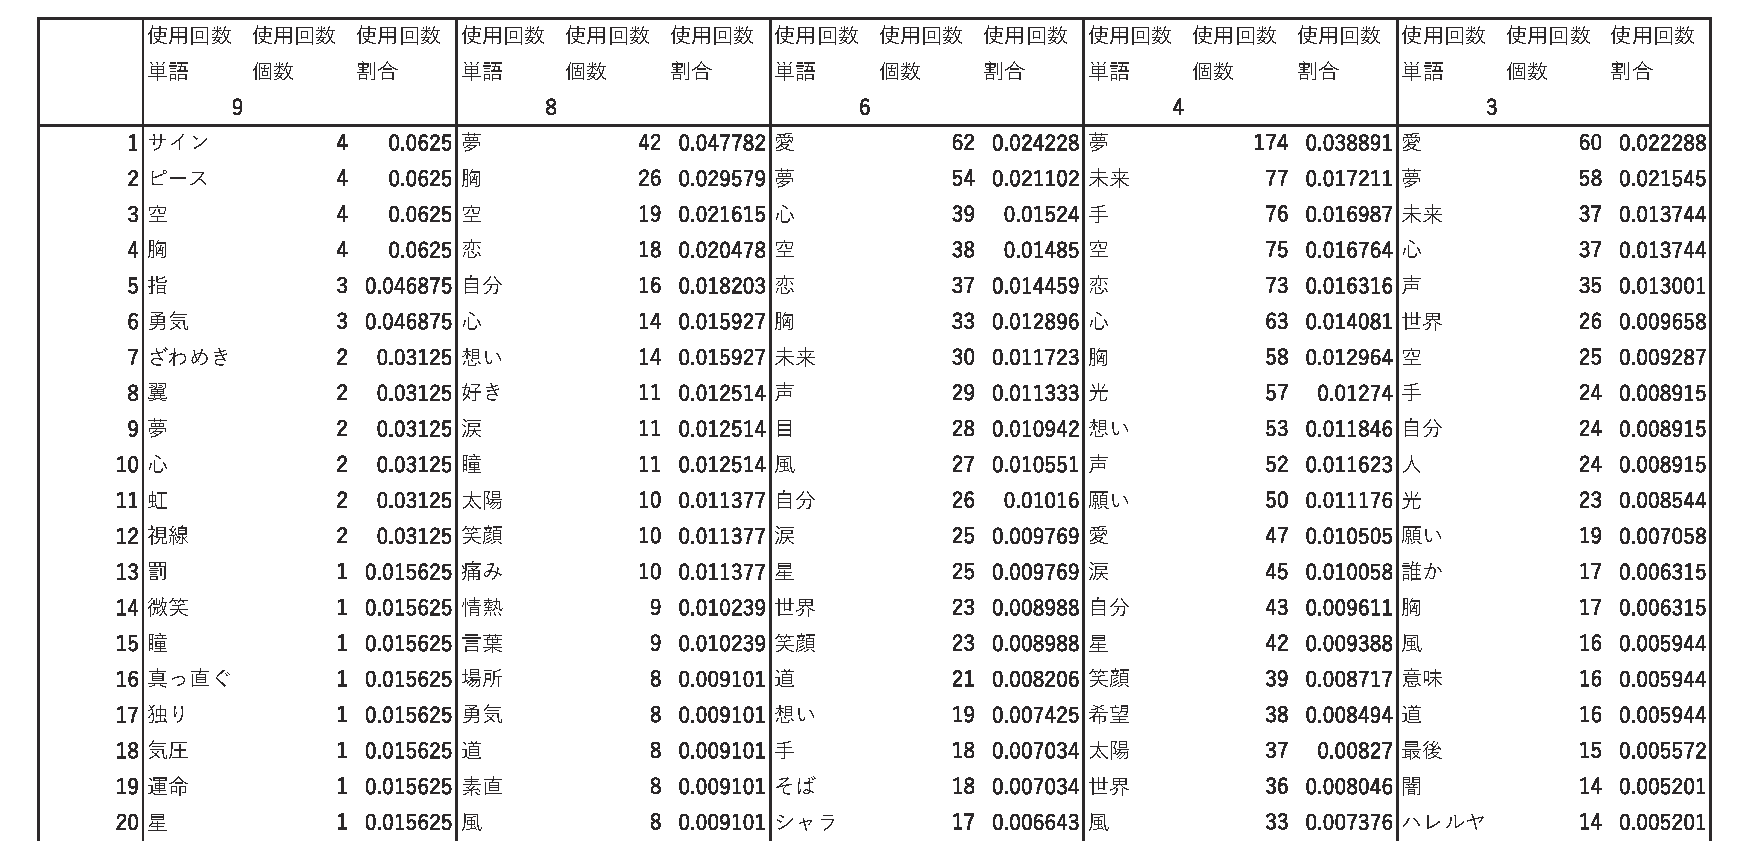
\includegraphics[width=\columnwidth]{fig/w-meishi-kaisu.pdf}
	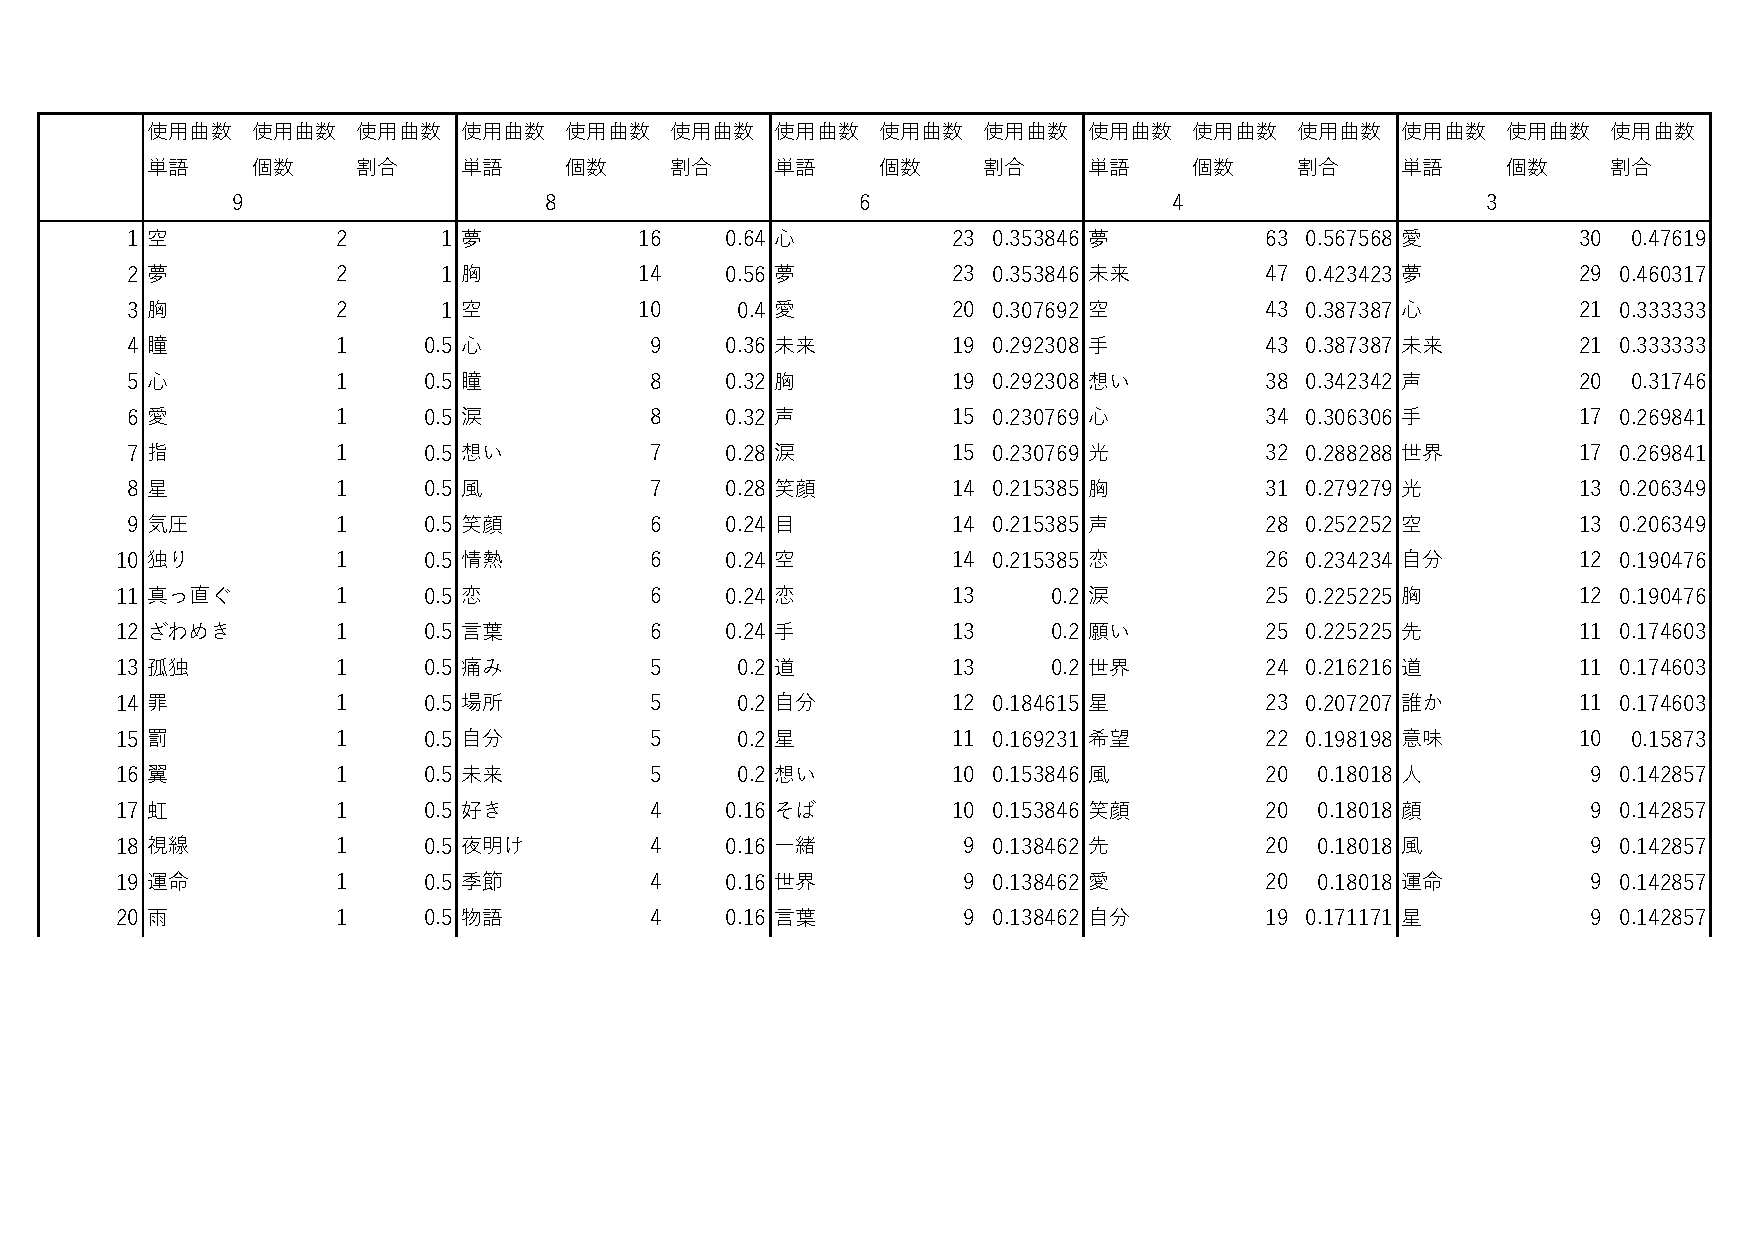
\includegraphics[width=\columnwidth]{fig/w-meishi-kyokusu.pdf}
	\caption{名詞の使用回数（上），使用曲数（下）}
	\label{fig:meishi}
\end{figure}



「夢」と「愛」が9人時代を除いた時代で1番，もしくは2番目に多い．また6人と比較して「未来」が急上昇しているように見える．


\begin{figure}[tb]
	\centering
	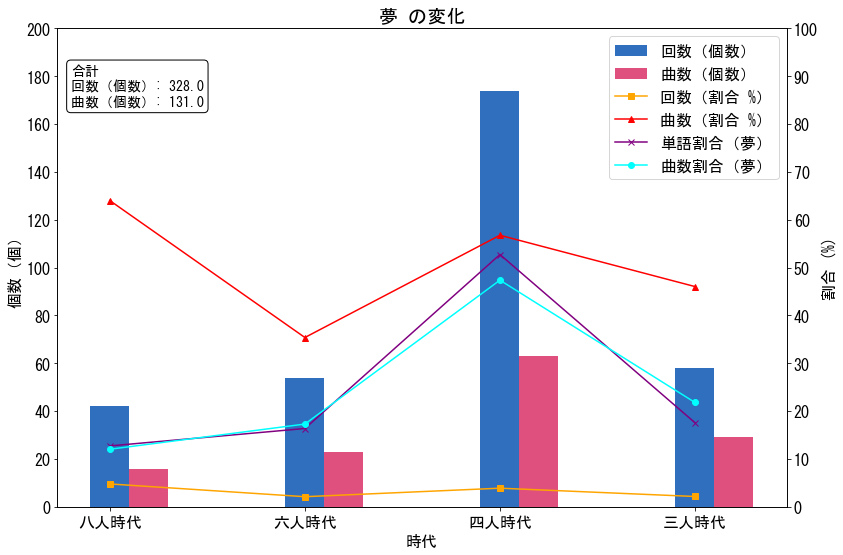
\includegraphics[width=\hsize]{fig/meishi-yume.png}
	\caption{「夢」の比較グラフ}
	\label{fig:yume}
	%\end{figure}
	%\begin{figure}[tb]
	\centering
	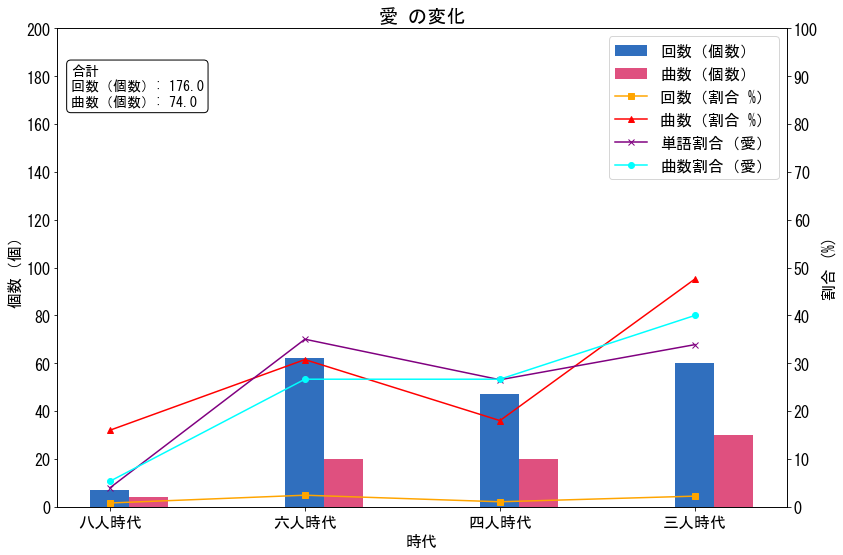
\includegraphics[width=\hsize]{fig/meishi-ai.png}
	\caption{「愛」の比較グラフ}
	\label{fig:ai}
	%\end{figure}
	%\begin{figure}[tb]
	\centering
	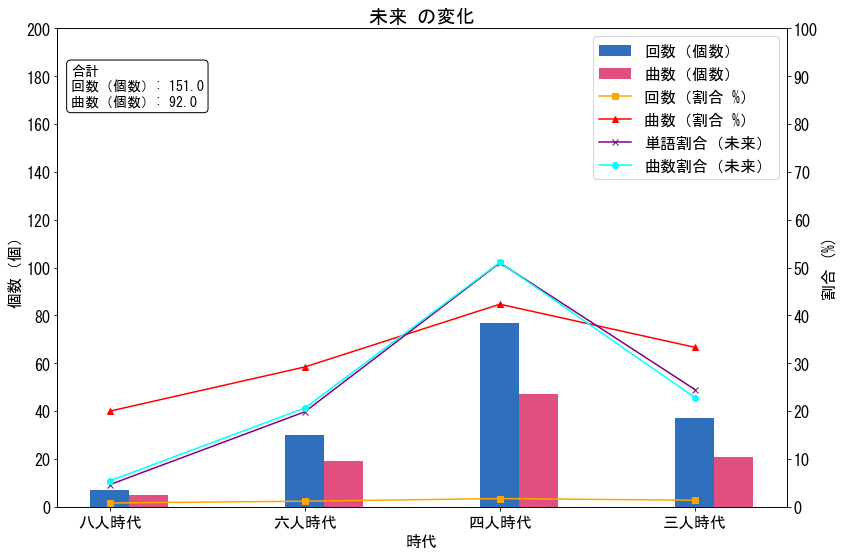
\includegraphics[width=\hsize]{fig/meishi-mirai.png}）
	\caption{「未来」の比較グラフ}
	\label{fig:mirai}
\end{figure}


「夢」は4人時代に突出して多いことがわかる（\figref{fig:yume}）．
「愛」は逆に4人時代は数が減っており一つの特徴といえるだろう（\figref{fig:ai}）．
「未来」は「夢」と同じく，4人時代に多い傾向が出た（\figref{fig:mirai}）．

\subsection{単語に注目した比較}
\protect\ref{sec:hinshi-suii}のうち，名詞と動詞においてより詳しく比較を行った．
ここまで単語の数だけで比較し特徴を調べてきたが．同じ単語でも楽曲内で使われ方は千差万別だ．そこで指定した単語を含む歌詞を抜き出し，辞書の意味に沿ってその楽曲内での単語の使われ方を筆者の主観で分類した．

その上で積み上げグラフと分類の内訳，割合を出している．割合に関しては小数点以下一桁丸め込んでいる．

名詞については，NEWSで最も使われていた「夢」と特徴的なグラフが出現した「愛」について詳しく比較を行った．

動詞については「行く」と「願う」について着目した．
「行く」はNEWSで最も使われた動詞であること，「願う」は4人で突出して使われていることからこの2単語で比較を行った．
動詞に関しては名詞のように単語そのものの辞書的な意味で分けるのではなく，「どこに行く」のか，「何を願う」のかで分類を行った．この分類の基準は筆者独自の判断で分けている．
また，動詞は活用形があるため使われ方によって形が変化する．そこで今回は漢字の「行」「願」を指定して抜き出している．


\subsubsection{「夢」の使われ方}
辞書の分類によると「夢」は以下の5種類に分類される\cite{yume}．

\begin{enumerate}
	\item 睡眠中に見る夢
	\item 将来実現させたい夢
	\item 現実からかけ離れた夢
	\item 心の迷い
	\item はかないこと
	\item 夢を含む単語
\end{enumerate}
を付け加えて分類した．

複数種類出てくるものについては
6と他の番号の場合は他の番号を割り振る．
6以外の番号同士の場合は楽曲の歌詞全体から判断した．

以下，\figref{fig:yume-ninzu}に分類した積み上げ棒グラフを，\protect\tabref{tab:yume-uchi}，\protect\tabref{tab:yume-wari}に内訳，割合の表を示す．

\begin{figure}[tb]
	\centering
	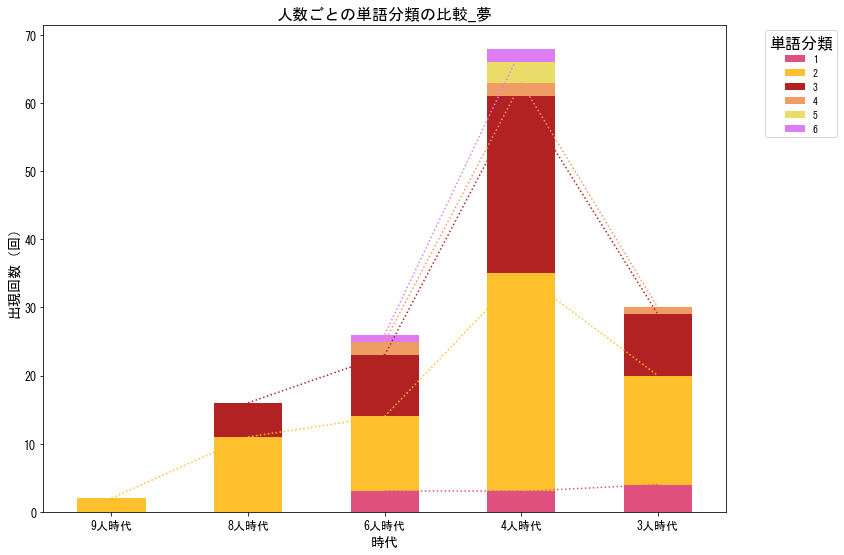
\includegraphics[width=\hsize]{fig/yume-ninzu.png}
	\caption{「夢」人数別時代ごとの分類比較グラフ}
	\label{fig:yume-ninzu}
\end{figure}

\begin{table}[tb]
	\centering
	\caption{「夢」人数別時代ごとの分類比較（内訳）}
	\label{tab:yume-uchi}
	\begin{tabular}{c|cccccc}
		\hline
		単語分類  & 9 & 8  & 6  & 4  & 3  & 合計（個） \\
		\hline\hline
		1     & 0 & 0  & 3  & 3  & 4  & 10    \\
		2     & 2 & 11 & 11 & 32 & 16 & 72    \\
		3     & 0 & 5  & 9  & 26 & 9  & 49    \\
		4     & 0 & 0  & 2  & 2  & 1  & 5     \\
		5     & 0 & 0  & 0  & 3  & 0  & 3     \\
		6     & 0 & 0  & 1  & 2  & 0  & 3     \\
		\hline\hline
		合計（個） & 2 & 16 & 26 & 68 & 30 & 142   \\
		\hline
		%「表の中身を書く」
	\end{tabular}
\end{table}

\begin{table}[tb]
	\centering
	\caption{「夢」人数別時代ごとの分類比較（割合）}
	\label{tab:yume-wari}
	\begin{tabular}{c|cccccc}
		\hline
		単語分類   & 9   & 8    & 6    & 4    & 3    & 合計（\%） \\
		\hline\hline
		1      & 0   & 0    & 11.5 & 4.4  & 13.3 & 7      \\
		2      & 100 & 68.8 & 42.3 & 47.1 & 53.3 & 50.7   \\
		3      & 0   & 31.2 & 34.6 & 38.2 & 30   & 34.5   \\
		4      & 0   & 0    & 7.7  & 2.9  & 3.3  & 3.5    \\
		5      & 0   & 0    & 0    & 4.4  & 0    & 2.1    \\
		6      & 0   & 0    & 3.8  & 2.9  & 0    & 2.1    \\
		\hline\hline
		合計（\%） & 100 & 100  & 100  & 100  & 100  & 100    \\
		\hline
		%「表の中身を書く」
	\end{tabular}
\end{table}




%\begin{figure}[tb]
%	\centering
%	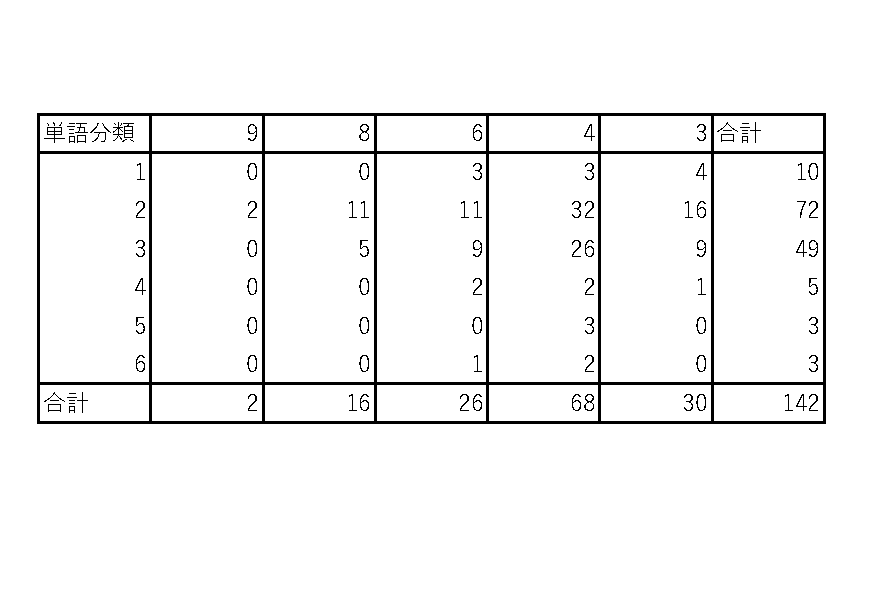
\includegraphics[width=\hsize]{fig/yume-uchi.pdf}
%	\caption{「夢」人数別時代ごとの単語分類比較（内訳）}
%	\label{fig:yume-uchi}
%\end{figure}
%\begin{figure}[tb]
%	\centering
%	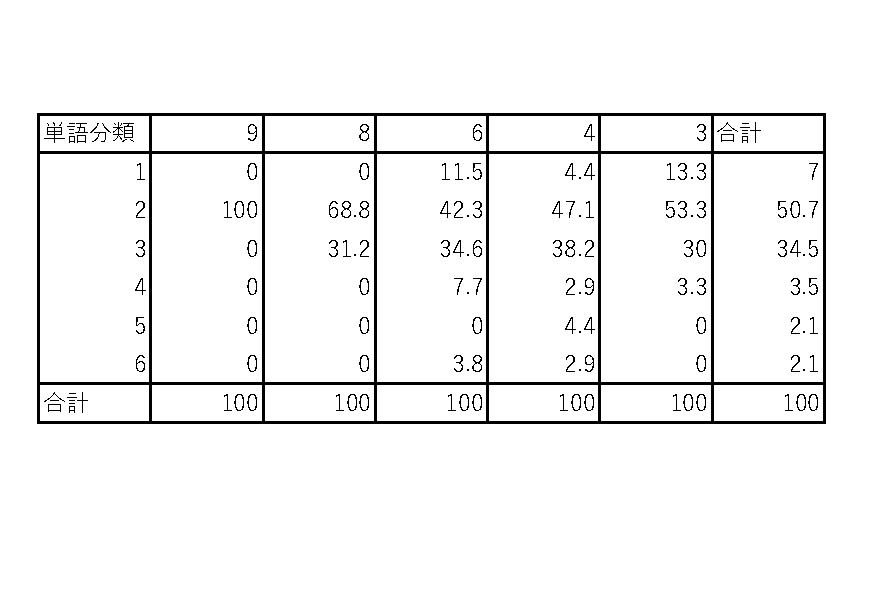
\includegraphics[width=\hsize]{fig/yume-wari.pdf}
%	\caption{「夢」人数別時代ごとの単語分類比較（割合）}
%	\label{fig:yume-wari}
%\end{figure}

睡眠中の「夢」をさす場合は少なく，半分以上が将来の「夢」について歌われていた．また，二番目に多かったのが現実からかけ離れた「夢」だった．
六人時代と四人時代の差では割合に着目すると将来の「夢」，現実からかけ離れた「夢」ともに少し割合が増えているものの，大きく増えたわけではないことが分かった．しかし，睡眠中の「夢」，そして心の迷いの「夢」として使われているものが六人時代と比較して四人時代のほうが大きく減っていることが分かった．
割合に着目すると大きな差はないように見えるが，「夢」が含まれる曲数では圧倒的に四人時代が多い．全体的な曲数が六人時代65曲，四人時代111曲，三人時代63曲であり，曲数と比率を比較すると四人時代が大きくなる，つまり他の時代と比べて四人時代は夢を多く歌っているといえる．

\subsubsection{「愛」の使われ方}
辞書の分類によると「愛」は以下の6種類に分類される\cite{AI}．
\begin{enumerate}
	\item 親子，兄弟などをいつくしみ合う気持ち
	\item 性愛の対象として特定の人をいとしいと思う心
	\item ある物事を好み，大切に思う気持ち
	\item 個人的な感情を超越した幸せを願う深く温かい心
	\item 他者を自分と同じようにいつくしむこと
	\item 自我の欲望に根ざし解脱を防げるもの
	\item 韻
	\item 愛が含まれる単語
\end{enumerate}
今回分類を進めると，「愛せ悔いなきな日々をI sayたゆまず歩もう（フィナーレ）」や「Fly highそれも深い愛（FLY HIGHT）」などのように韻として使われている場合と
動詞として使用されている場合があった．
ここでは動詞は比較対象外なので除外している．
また，5，6の意味に関しては出現しんなかったため省いている．

以下，\figref{fig:ai-ninzu}に分類した積み上げ棒グラフを，\protect\tabref{tab:ai-uchi}，\protect\tabref{tab:ai-wari}に内訳，割合の表を示す．

\begin{figure}[tb]
	\centering
	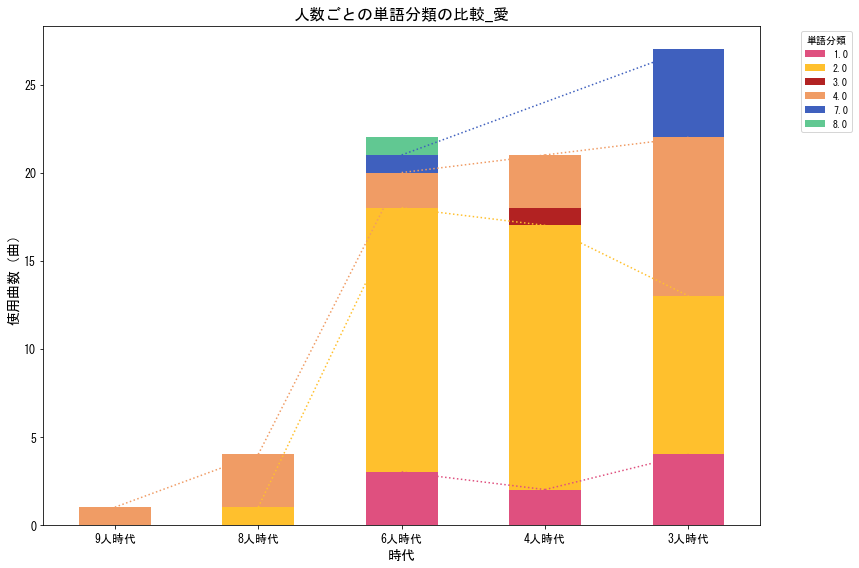
\includegraphics[width=\hsize]{fig/ai-ninzu.png}
	\caption{「愛」人数別時代ごとの分類比較グラフ}
	\label{fig:ai-ninzu}
\end{figure}



\begin{table}[tb]
	\centering
	\caption{「愛」人数別時代ごとの分類比較（内訳）}
	\label{tab:ai-uchi}
	\begin{tabular}{c|cccccc}
		\hline
		単語分類  & 9 & 8 & 6  & 4  & 3  & 合計（個） \\
		\hline\hline
		1     & 0 & 0 & 3  & 2  & 4  & 9     \\
		2     & 0 & 1 & 15 & 15 & 9  & 40    \\
		3     & 0 & 0 & 0  & 1  & 0  & 1     \\
		4     & 1 & 3 & 2  & 3  & 9  & 18    \\
		7     & 0 & 0 & 1  & 0  & 5  & 6     \\
		8     & 0 & 0 & 1  & 0  & 0  & 1     \\
		\hline\hline
		合計（個） & 1 & 4 & 22 & 21 & 27 & 75    \\
		\hline
		%「表の中身を書く」
	\end{tabular}
\end{table}

\begin{table}[tb]
	\centering
	\caption{「愛」人数別時代ごとの分類比較（割合）}
	\label{tab:ai-wari}
	\begin{tabular}{c|cccccc}
		\hline
		単語分類   & 9   & 8   & 6    & 4    & 3    & 合計（\%） \\
		\hline\hline
		1      & 0   & 0   & 13.6 & 9.5  & 14.8 & 12     \\
		2      & 0   & 25  & 68.2 & 71.4 & 33.3 & 53.3   \\
		3      & 0   & 0   & 0    & 4.8  & 0    & 1.3    \\
		4      & 100 & 75  & 9.1  & 14.3 & 33.3 & 24     \\
		7      & 0   & 0   & 4.5  & 0    & 18.5 & 8      \\
		8      & 0   & 0   & 4.5  & 0    & 0    & 1.3    \\
		\hline\hline
		合計（\%） & 100 & 100 & 100  & 100  & 100  & 100    \\
		\hline
		%「表の中身を書く」
	\end{tabular}
\end{table}





%\begin{figure}[tb]
%	\centering
%	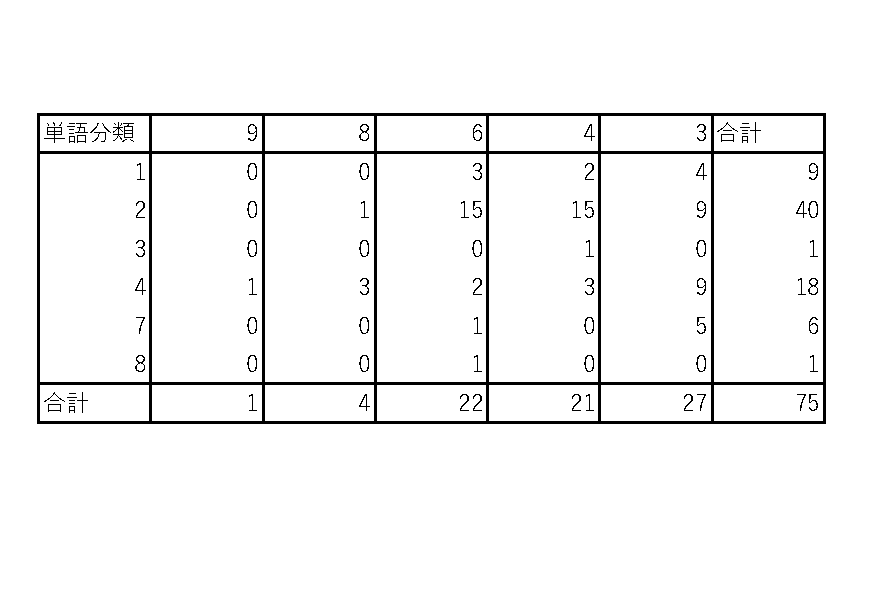
\includegraphics[width=\hsize]{fig/ai-uchi.pdf}
%	\caption{「愛」人数別時代ごとの単語分類比較（内訳）}
%	\label{fig:yume-uchi}
%\end{figure}
%\begin{figure}[tb]
%	\centering
%	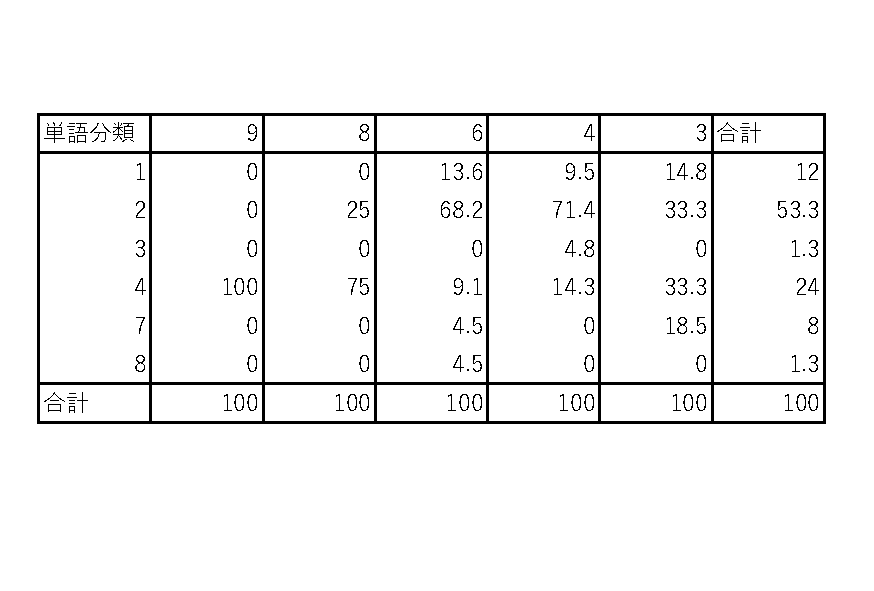
\includegraphics[width=\hsize]{fig/ai-wari.pdf}
%	\caption{「愛」人数別時代ごとの単語分類比較（割合）}
%	\label{fig:yume-wari}
%\end{figure}

全体的に性愛の対象として特定の人をいとしいと思う心，個人的な感情を超越した幸せを願う深く温かい心が多く出現した．


\subsubsection{「行（く）」の使われ方}
今回は以下の9種類に分類した．
\begin{enumerate}
	\item　未来，希望
	\item　具体的な行先
	\item　宇宙，星など
	\item　概念的なもの
	\item　行先未定
	\item　行くぞ！（呼びかけ）
	\item　歌詞としての呼びかけ
	\item　単語
	\item　その他
\end{enumerate}

以下，\figref{fig;iku-ninzu}に分類した積み上げ棒グラフを，\protect\tabref{tab:iku-uchi}，\protect\tabref{tab:iku-wari}に内訳，割合の表を示す．

\begin{figure}[tb]
	\centering
	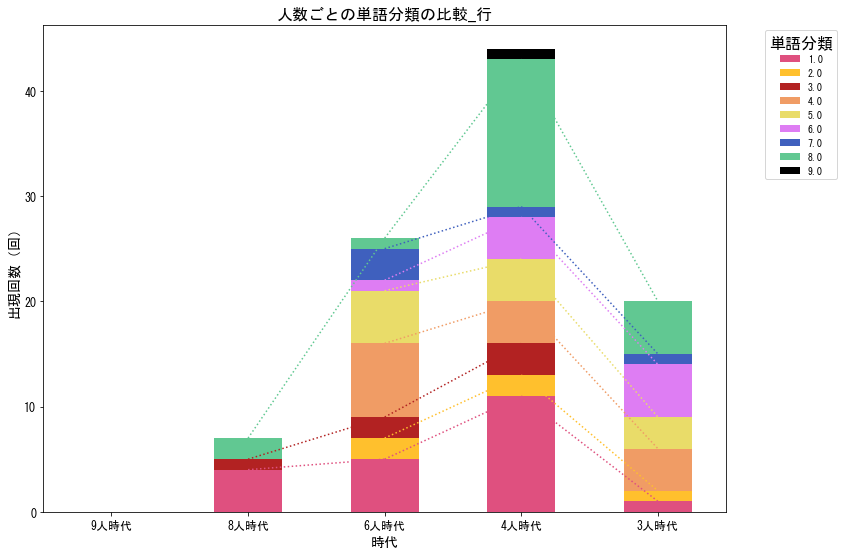
\includegraphics[width=\hsize]{fig/iku-ninzu.png}
	\caption{「行」人数別時代ごとの分類比較グラフ}
	\label{fig;iku-ninzu}
\end{figure}


\begin{table}[tb]
	\centering
	\caption{「行」人数別時代ごとの分類比較（内訳）}
	\label{tab:iku-uchi}
	\begin{tabular}{c|ccccc}
		\hline
		単語分類  & 8 & 6  & 4  & 3  & 合計（個） \\
		\hline\hline
		1     & 4 & 5  & 11 & 1  & 21    \\
		2     & 0 & 2  & 2  & 1  & 5     \\
		3     & 1 & 2  & 3  & 0  & 6     \\
		4     & 0 & 7  & 4  & 4  & 15    \\
		5     & 0 & 5  & 4  & 3  & 12    \\
		6     & 0 & 1  & 4  & 5  & 10    \\
		7     & 0 & 3  & 1  & 1  & 5     \\
		8     & 2 & 1  & 14 & 5  & 22    \\
		9     & 0 & 0  & 1  & 0  & 1     \\
		\hline\hline
		合計（個） & 7 & 26 & 44 & 20 & 97    \\
		\hline
		%「表の中身を書く」
	\end{tabular}
\end{table}

\begin{table}[tb]
	\centering
	\caption{「行」人数別時代ごとの分類比較（割合）}
	\label{tab:iku-wari}
	\begin{tabular}{c|ccccc}
		\hline
		単語分類   & 8    & 6    & 4    & 3   & 合計（\%） \\
		\hline\hline
		1      & 57.1 & 19.2 & 25   & 5   & 21.6   \\
		2      & 0    & 7.7  & 4.5  & 5   & 5.2    \\
		3      & 14.3 & 7.7  & 6.8  & 0   & 6.2    \\
		4      & 0    & 26.9 & 9.1  & 20  & 15.5   \\
		5      & 0    & 19.2 & 9.1  & 15  & 12.4   \\
		6      & 0    & 3.8  & 9.1  & 25  & 10.3   \\
		7      & 0    & 11.5 & 2.3  & 5   & 5.2    \\
		8      & 28.6 & 3.8  & 31.8 & 25  & 22.7   \\
		9      & 0    & 0    & 2.3  & 0   & 1      \\
		\hline\hline
		合計（\%） & 100  & 100  & 100  & 100 & 100    \\
		\hline
		%「表の中身を書く」
	\end{tabular}
\end{table}


% \begin{figure}[tb]
%	\centering
%	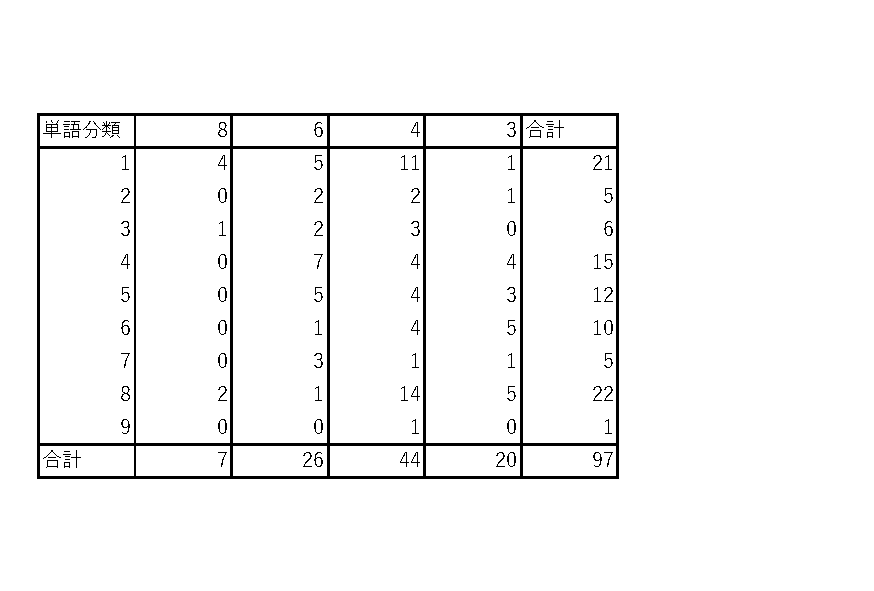
\includegraphics[width=\hsize]{fig/iku-uchi.pdf}
%	\caption{「行」人数別時代ごとの単語分類比較（内訳）}
%	\label{fig:iku-uchi}
%\end{figure}
%\begin{figure}[tb]
%	\centering
%	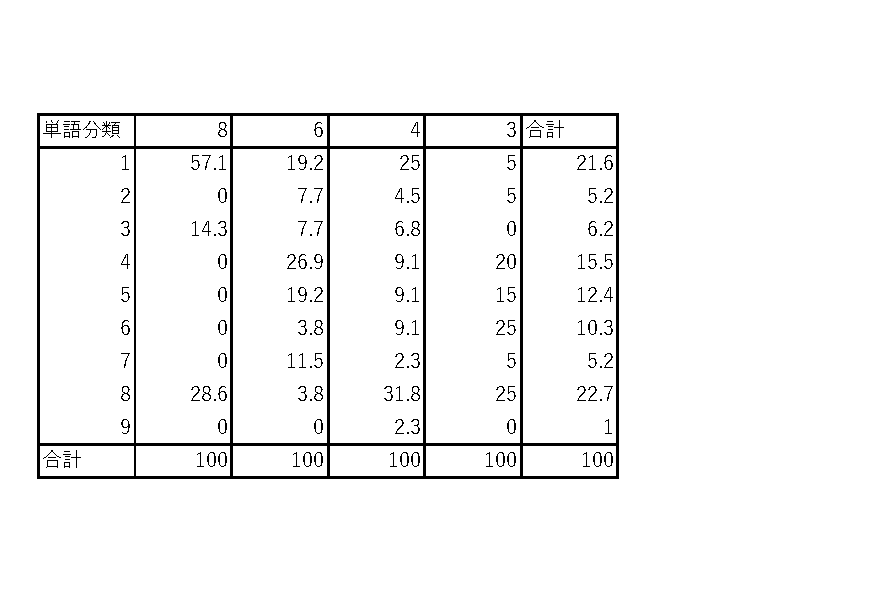
\includegraphics[width=\hsize]{fig/iku-wari.pdf}
%	\caption{「行」人数別時代ごとの単語分類比較（割合）}
%	\label{fig:iku-wari}
%\end{figure}

具体的な行先を指定するよりも4,5の概念的なものや行先未定のものが多い結果となった．概念的なという意味では似ているが未来や希望に向かっていく表現のものが多く，特に六人時代から四人時代で大きく増えたわけではないが増えていることが確認できる．

\subsubsection{「願（う）」の使われ方}
今回は以下の6種類に分類した
\begin{enumerate}
	\item 未来，希望
	\item 恋，恋愛系
	\item 過去
	\item 相手に願う
	\item 勝利
	\item 愛
	\item 音楽
\end{enumerate}

以下，\figref{fig:negau-ninzu}に分類した積み上げ棒グラフを，\protect\tabref{tab:negau-uchi}，\protect\tabref{tab:negau-wari}に内訳，割合の表を示す．

\begin{figure}[tb]
	\centering
	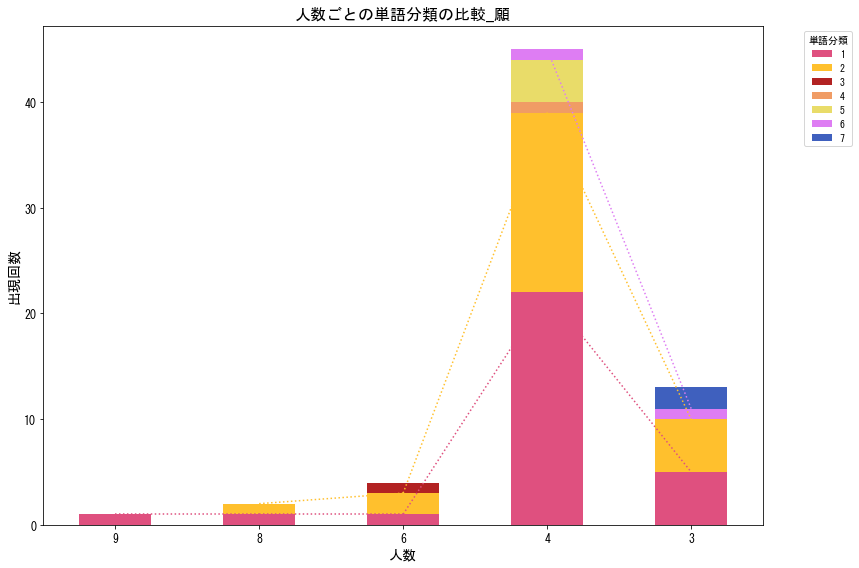
\includegraphics[width=\hsize]{fig/negau-ninzu.png}
	\caption{「願」人数別時代ごとの分類比較グラフ}
	\label{fig:negau-ninzu}
\end{figure}

\begin{table}[tb]
	\centering
	\caption{「願」人数別時代ごとの分類比較（内訳）}
	\label{tab:negau-uchi}
	\begin{tabular}{c|cccccc}
		\hline
		単語分類  & 9 & 8 & 6 & 4  & 3  & 合計（個） \\
		\hline\hline
		1     & 1 & 1 & 1 & 22 & 5  & 30    \\
		2     & 0 & 1 & 2 & 17 & 5  & 25    \\
		3     & 0 & 0 & 1 & 0  & 0  & 1     \\
		4     & 0 & 0 & 0 & 1  & 0  & 1     \\
		5     & 0 & 0 & 0 & 4  & 0  & 4     \\
		6     & 0 & 0 & 0 & 1  & 1  & 2     \\
		7     & 0 & 0 & 0 & 0  & 2  & 2     \\
		\hline\hline
		合計（個） & 1 & 2 & 4 & 45 & 13 & 65    \\
		\hline
		%「表の中身を書く」
	\end{tabular}
\end{table}

\begin{table}[tb]
	\centering
	\caption{「願」人数別時代ごとの分類比較（割合）}
	\label{tab:negau-wari}
	\begin{tabular}{c|cccccc}
		\hline
		単語分類   & 9   & 8   & 6   & 4    & 3    & 合計（\%） \\
		\hline\hline
		1      & 100 & 50  & 25  & 48.9 & 38.5 & 46.2   \\
		2      & 0   & 50  & 50  & 37.8 & 38.5 & 38.5   \\
		3      & 0   & 0   & 25  & 0    & 0    & 1.5    \\
		4      & 0   & 0   & 0   & 2.2  & 0    & 1.5    \\
		5      & 0   & 0   & 0   & 8.9  & 0    & 6.2    \\
		6      & 0   & 0   & 0   & 2.2  & 7.7  & 3.1    \\
		7      & 0   & 0   & 0   & 0    & 15.4 & 3.1    \\
		\hline\hline
		合計（\%） & 100 & 100 & 100 & 100  & 100  & 100    \\
		\hline
		%「表の中身を書く」
	\end{tabular}
\end{table}

%\begin{figure}[tb]
%	\centering
%	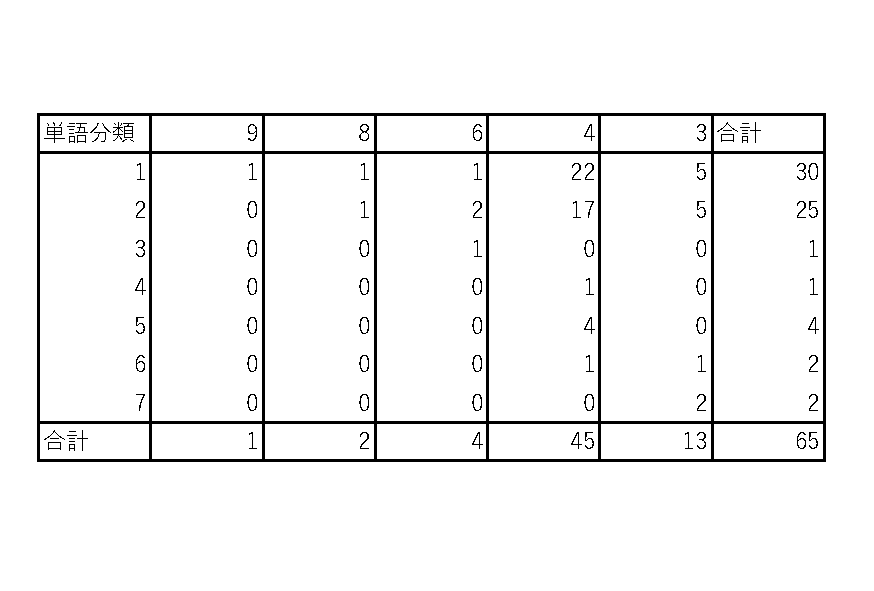
\includegraphics[width=\hsize]{fig/negau-uchi.pdf}
%	\caption{「願」人数別時代ごとの分類比較（内訳）}
%	\label{fig:yume-uchi}
%\end{figure}
%\begin{figure}[tb]
%	\centering
%	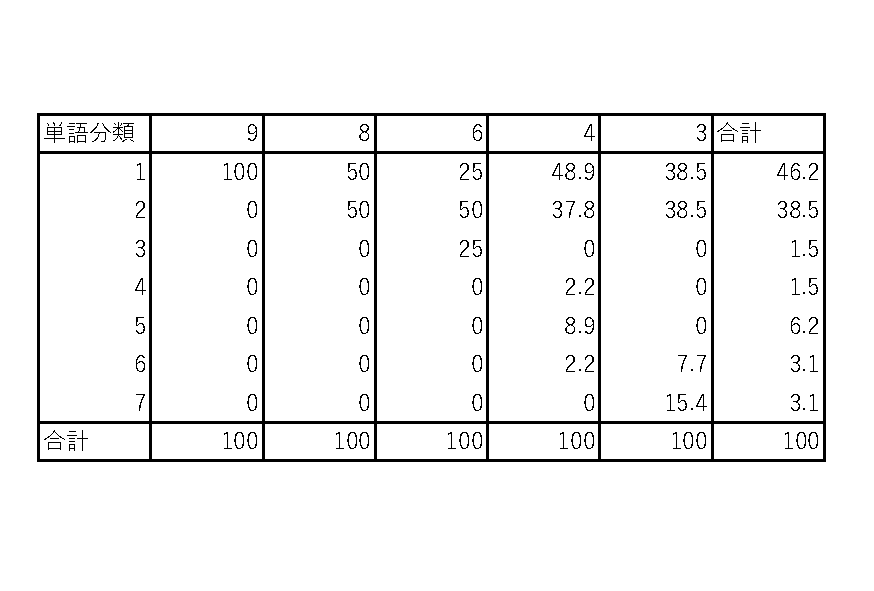
\includegraphics[width=\hsize]{fig/negau-wari.pdf}
%	\caption{「願」人数別時代ごとの分類比較（割合）}
%	\label{fig:yume-wari}
%\end{figure}

六人時代と比較して四人時代は未来，希望に関する使われ方が圧倒的に多いことがわかる．逆に恋，恋愛系に関する使われ方は減っていた．六人時代と四人時代で明確に使われ方が分かれる結果となり，それぞれの時代の違いといえるだろう．


\subsubsection{まとめ}
特定の単語に着目してその単語の使用用途について比較した．
「夢」はどの時代を通しても将来実現させたい「夢」を歌っていた．
「愛」は他の時代で恋愛的な使われ方が最も多いのに対し，三人時代は個人的な感情を超越した幸せを願う温かい心と同率となっており時代別の使われ方で違いが確認できた．
「行く」は未来や希望に向かって使われていることが多く，具体的な行き先が設定されているよりも概念的な行先に使われていることが多かった．
「願う」は六人時代と四人時代で最も多い使われ方が違った．恋愛系に使われることが最も多かった6人時代，未来や希望に対して使われることが最も多い四人時代となった．また三人時代はこの二項目が同率となり時代ごとに使われ方が最も変わったといえる．
このことから単語によって差はあるものの時代ごとに使われ方に違いがあることが分かった．



\section{キーワード別の楽曲分析}\label{sec:words}

筆者はNEWS楽曲の傾向として大きく2つのキーワードを設定した．一つは「背中を押された」もう一つは「エモーショナルさ」である．前者は公式アカウントで言及されており，後者はメンバー本人からの発言であった．
そこでこのキーワードをもとに楽曲を選曲し，そのデータごとに品詞分析を行う．このうちで上位にある単語を全楽曲の年代別に照らし合わせる．これにより特定のキーワードを示す単語がいつごろから増えたのか特定すること目的として5章にて分析を行う．
手順として，まずキーワードに基づく選曲を行いデータを作る．そしてそのデータ群で最も使用されている単語に着目し，その単語がNEWSの活動した時系列でどのように増えたのかを年ごとの累積グラフで確認する．


\subsection{\senaka 楽曲の比較}



\subsubsection{NEWSの「背中を押す」楽曲の比較}

%第１章より
彼らを応援している中で，「NEWSは背中を押してくれる楽曲が多い」といった声を聴くことがあった．そしてそのような印象を持つ楽曲は2012年以降に発表された楽曲が多いと感じている．実際，公式アカウントでグループを紹介する際には「多くの人の背中を押してきた」\cite{NEWS_Chill}と書かれていた．ほかにもドキュメンタリー\cite{Ongaku}内でメンバーが「エモーショナルさがNEWSの魅力になってきている」と発言しており，そこに挙げられた楽曲はどれも2012年以降に発表されたものだった．


ここではNEWS楽曲のうち「背中を押す」をキーワードに楽曲を絞った．
対象としたのは筆者自身が「背中を押された」と感じた楽曲35曲である．

\protect\tabref{tab:news-senaka}に選曲した35曲の名詞使用回数上位10単語の表を，
\figref{fig:top10-news-senaka-ruiseki}に\protect\tabref{tab:news-senaka}をもとにした全楽曲の累積グラフを示す．

\begin{table}[tb]
	\centering
	\caption{選曲した35曲の名詞使用回数上位10単語}
	\label{tab:news-senaka}
	\begin{tabular}{c|c}
		\hline
		単語 & 使用回数 \\ \hline
		夢  & 79   \\
		自分 & 54   \\
		未来 & 35   \\
		涙  & 34   \\
		心  & 32   \\
		空  & 30   \\
		笑顔 & 26   \\
		胸  & 23   \\
		声  & 22   \\
		道  & 20   \\
		\hline

		%「表の中身を書く」
	\end{tabular}
\end{table}

%図
%\begin{figure}[tb]
%	%\centering
%	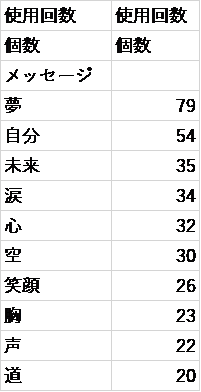
\includegraphics[width=45mm]{fig/top10-news-senaka.png}
%	\caption{	選曲した35曲の名詞使用回数上位10}
%	\label{fig:top10-news-senaka-hyou}
%\end{figure}
\begin{figure}[tb]
	\centering
	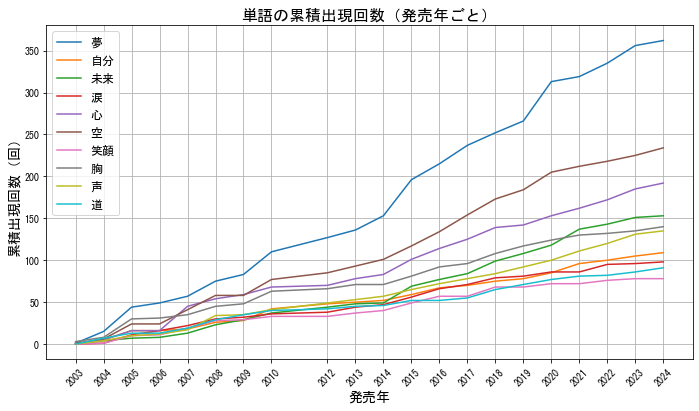
\includegraphics[width=\hsize]{fig/top10-news-senaka-ruiseki.png}
	\caption{\protect\tabref{tab:news-senaka}をもとにした全楽曲の累積グラフ}
	\label{fig:top10-news-senaka-ruiseki}
\end{figure}

最も多い「夢」だが，顕著に上がっている時期は2004-2005，2009-2010，2014-2015，2020-2021と見た．
その他のグラフも2015年を境に角度が上がっており，使用される回数が増えている．このことからNEWSにとって2015年あたりが楽曲の歌詞傾向が変化したタイミングなのではないかと考える．


\subsubsection{一般的な「背中を押す」楽曲との比較}
\paragraph*{アンケート調査}
キーワードごとの選曲のうち，「背中を押された」楽曲に関してはアンケートを実施した．
以下にアンケートの概要をまとめる．

\begin{enumerate}
	\item \textbf{目的}
	      \senaka 楽曲の歌詞について広く募集し，NEWS以外の視点から分析を行うことを目的とする．また，「背中を押された」という表現には似たような感覚が多くあると考えられた．そのため，今回のアンケートでは「勇気をもらった」「励まされた」など，似たような感覚であってもよいものとした．

	\item \textbf{調査期間}
	      2024年10月21日から2024年10月30日まで

	\item \textbf{調査対象}
	      \begin{enumerate}
		      \item 橋田ゼミのメンバー
		      \item 音情報処理受講者
		      \item ヒューマンインタフェース受講者
		      \item メディア情報学受講者
	      \end{enumerate}

	\item \textbf{調査方法}
	      Googleフォームによる選択および記述回答

	\item \textbf{回収状況}
	      40件の回答を得られた．

	\item \textbf{結果}

	      \begin{figure}[h]
		      \centering
		      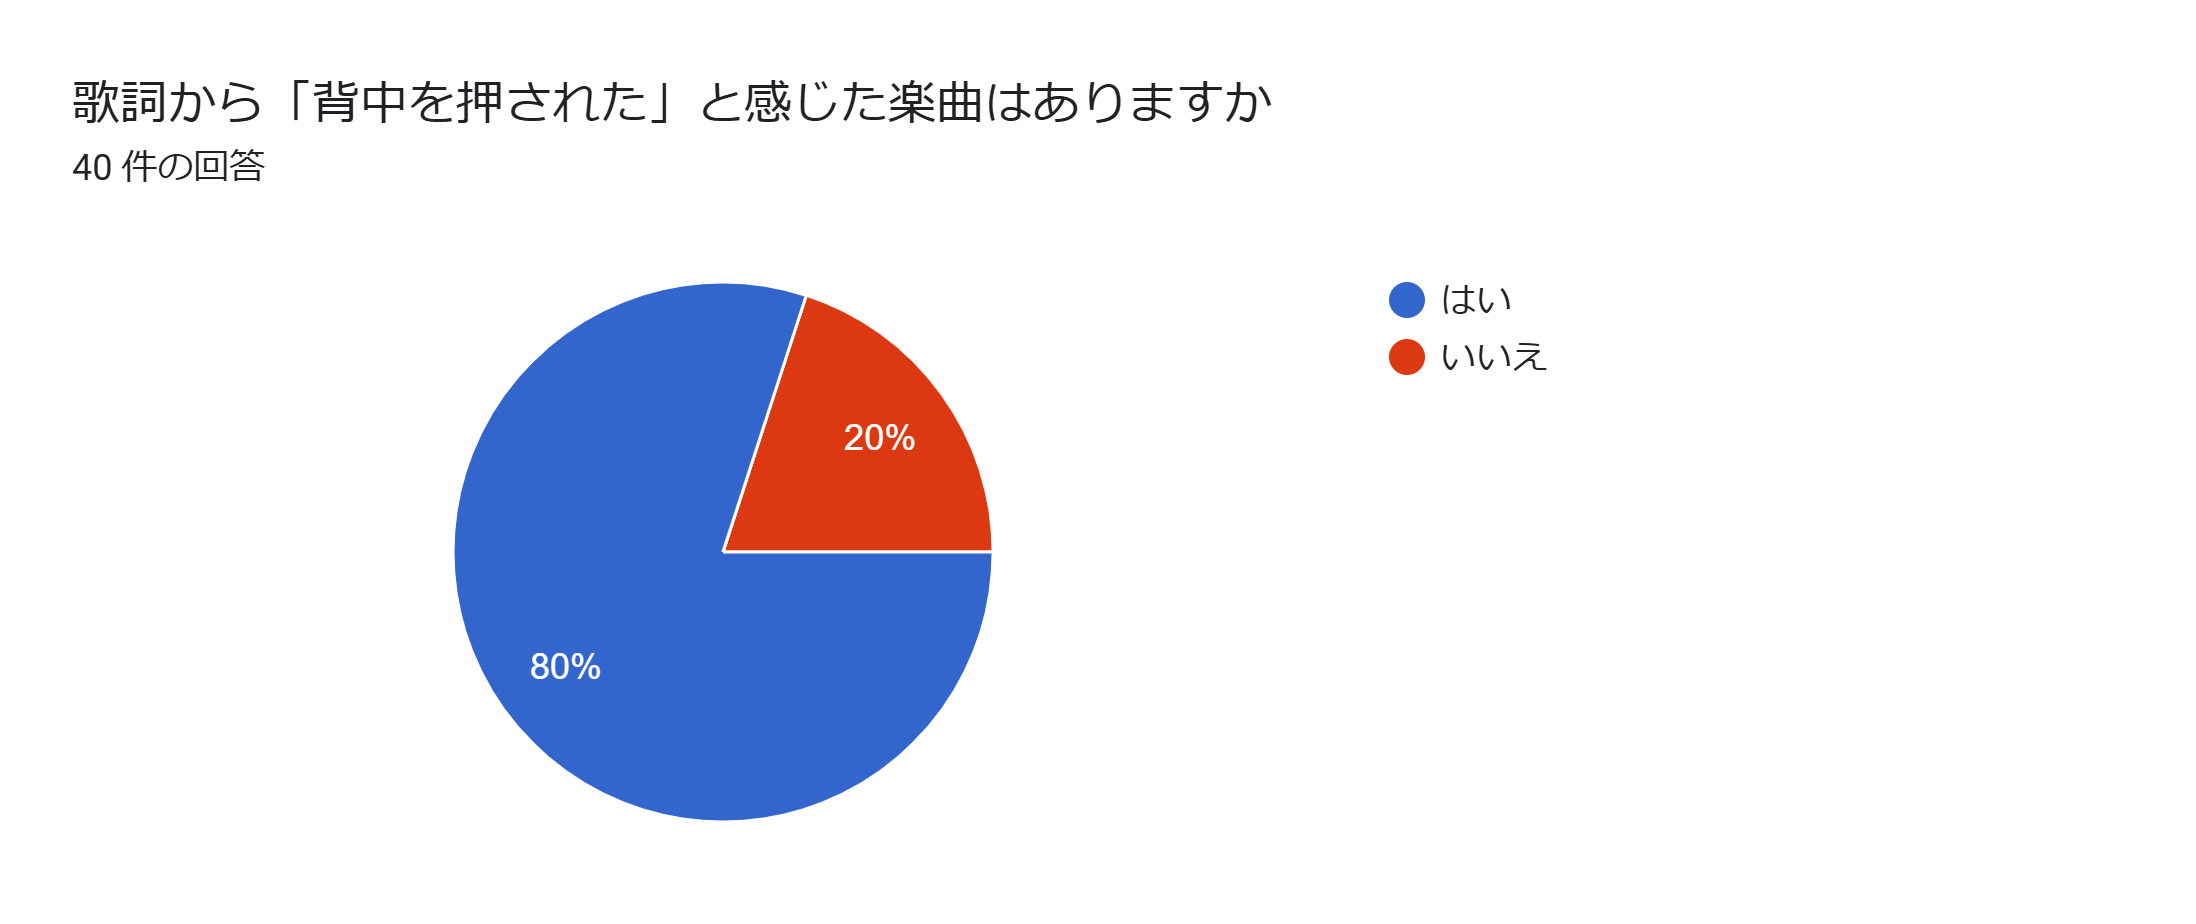
\includegraphics[width=\hsize]{fig/senaka-anke.png}
		      \caption{アンケート結果}
		      \label{fig:senaka-anke}
	      \end{figure}

	      八割の人が歌詞から「背中を押された」と感じた楽曲がある結果となった（\figref{fig:senaka-anke}）．

\end{enumerate}


今回実施したアンケート内で「背中を押された」楽曲名を挙げてもらったのだが，特に歌詞のどの部分で「背中を押された」のかも書いてもらった．この実際に「背中を押された」歌詞部分に着目し，NEWS以外の楽曲で「背中を押された」と感じる歌詞はNEWSでどのような増加傾向があるのかを確認する．

\protect\tabref{tab:ippan-senaka}にアンケート結果から得たデータの名詞上位10単語の表を，
\figref{fig:top10-ippan-ruiseki}に\protect\tabref{tab:ippan-senaka}をもとにした全楽曲の累積グラフを示す．

\begin{table}[tb]
	\centering
	\caption{アンケート結果から得たデータの名詞上位10単語}
	\label{tab:ippan-senaka}
	\begin{tabular}{c|c}
		\hline
		単語 & 使用回数 \\
		\hline
		心  & 11   \\
		世界 & 9    \\
		自分 & 7    \\
		無駄 & 5    \\
		涙  & 4    \\
		道  & 4    \\
		子供 & 4    \\
		だめ & 4    \\
		旅  & 4    \\
		不安 & 4    \\
		\hline

		%「表の中身を書く」
	\end{tabular}
\end{table}


%\begin{figure}[tb]
%	\centering
%	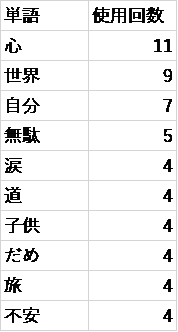
\includegraphics[width=45mm]{fig/top10-ippan-senaka.png}
%	\caption{	選曲した35曲の名詞使用回数上位10}
%	\label{fig:top10-ippan-hyou}
%\end{figure}
\begin{figure}[tb]
	\centering
	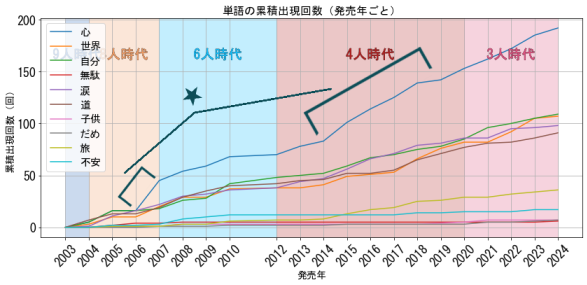
\includegraphics[width=\hsize]{fig/top10-ippan-senaka-ruiseki.png}
	\caption{\protect\tabref{tab:ippan-senaka}をもとにした全楽曲の累積グラフ}
	\label{fig:top10-ippan-ruiseki}
\end{figure}

大きく三つに分かれたのが印象的だ．
まず「心」だがこれは2006-2007，つまり六人時代から大きく増えていることがわかる．また2014-2015を境にまた増えていることが確認できた．
次に「世界」「自分」「涙」「道」の四つがあげられる．「続き」
最後に「旅」「不安」「子供」「だめ」「無駄」だが，否定的な単語が集まっている．このような単語が低頻度で出現していたということはNEWS楽曲の歌詞でネガティブな単語は少ない傾向にあるのではないかと推測する．


\subsection{「エモーショナルさ」のある楽曲の比較}
ここでは「エモーショナルさ」に着目して分析を行う．

%エモーショナルとは「強く感情に訴えるさま」という意味がある（出典）。NEWSの場合この「感情に訴えるさま」が「背中を押す」感覚につながったのではないだろうか．

今回「エモーショナルさ」の基準にしたのは「「“NEWS”と“音楽”」-Interview  \& Human Documentary- KOYAMA×KATO / KOYAMA×MASUDA」\cite{Ongaku}」でメンバーの加藤が発言していた5つの楽曲を対象とした．

\protect\tabref{tab:news-emo}に「エモーショナルさ」をもとに選曲したデータの名詞上位10単語の表を，
\figref{fig:top10-news-emo-ruiseki}に\protect\tabref{tab:news-emo}をもとにした全楽曲の累積グラフを示す．

\begin{table}[tb]
	\centering
	\caption{「エモーショナルさ」をもとに選曲したデータの名詞上位10単語}
	\label{tab:news-emo}
	\begin{tabular}{c|c}
		\hline
		単語     & 使用回数 \\
		\hline
		夢      & 11   \\
		自分     & 11   \\
		声      & 7    \\
		未来     & 7    \\
		愛      & 6    \\
		本当     & 6    \\
		願い     & 5    \\
		フルスイング & 5    \\
		意味     & 5    \\
		絆      & 4    \\
		\hline

		%「表の中身を書く」
	\end{tabular}
\end{table}


%\begin{figure}[tb]
%	\centering
%	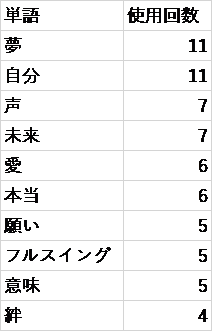
\includegraphics[width=45mm]{fig/top10-news-emo.png}
%	\caption{	選曲した35曲の名詞使用回数上位10}
%	\label{fig:top10-news-emo-hyou}
%\end{figure}
\begin{figure}[tb]
	\centering
	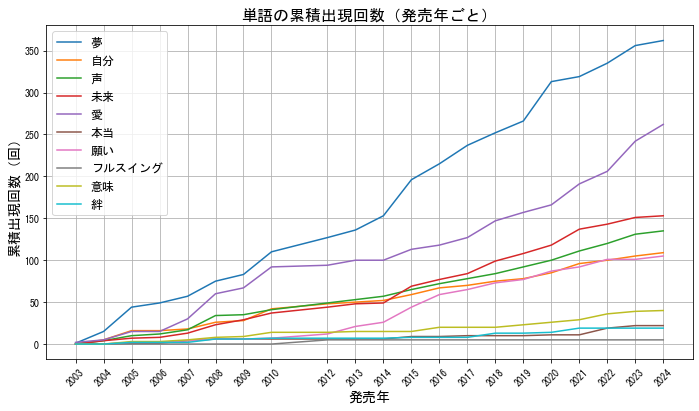
\includegraphics[width=\hsize]{fig/top10-news-emo-ruiseki.png}
	\caption{\protect\tabref{tab:news-emo}をもとにした全楽曲の累積グラフ}
	\label{fig:top10-news-emo-ruiseki}
\end{figure}

「夢」に関してはデビュー当初から増加傾向にあり，顕著に増加するタイミングは前述のとおりである．
「愛」は2007-2010のタイミングで最も増えている．これは六人時代の活動期と被っており，六人時代に増加したことが確認できる．
「願い」は2012年のタイミングから増加傾向にある．これは四人時代が始まった年なのでこの時代から増えたといえるだろう．
また，「未来」と上記三つの単語が2014-2015を境に増加しているように見える．このことからNEWSにとって2015年が歌詞の傾向として一つの転換点なのではないかと考えた．

\section{考察}


\subsection{時代別の歌詞分析に関する考察}
品詞分析から頻出語彙に着目した分析を行った．そして，使用単語の使われ方には人数ごとの違いが表れていることが分かった．
六人時代までと比較して四人時代や三人時代のほうが未来や希望に対して使われている傾向があり，NEWSが歌う楽曲の歌詞は前向きなものが増えているといえるだろう．
4章の初めに六人時代と四人時代で大きな差が生まれるのではないかと仮説を立てた．確かに四人時代以降は単語を未来や希望に対して歌っている楽曲は増えており，六人時代は恋愛に関する使われ方が多かった．ここがエモーショナルさにつながるのかはもっと別の角度からの考察をするべきだが，人数時代による変化を確認することはできた．
筆者の感覚なのだが，六人時代と四人時代の楽曲の雰囲気差は前々から感じていたものの，分析前までは四人時代と三人時代の差の特徴を明確に感じ切れていなかった．少し恋愛ソングが減ったような気がする程度だったのだが，今回「愛」の使われ方が個人ではなくより大きな存在になっていることが分かった．つまり三人時代はより普遍的な愛を歌っていた．
未来に関することが増えていた四人時代，普遍的な愛をうたうことが増えた三人時代．恋愛的な愛をうたっていた六人時代は歌詞内で対象となる一人がいる傾向にあると考えられる．しかし四人時代以降対象となる存在が自分を含めた大きなものへと変化している．これがエモーショナルさにつながるとは言い切れないが，単語の対象の変化は楽曲を受け止める印象の変化につながると考えた．

\subsection{キーワードごとの選曲に関する考察}

興味深い点として2015を境に注目した単語数が増えがちであるという点がある．このことからNEWSにとって2015とは一つの転換期であると思われる．
NEWSの音楽の方向性として筆者が挙げてきた転換点は六人時代と四人時代の境である2012以降だと仮説を立てていたが今回の分析では2015年のほうに差があると感じられた．AppleMusic の「NEWSについて」内で「『NEVERLAND』（2017年）では，より明確なコンセプトを打ち出すようになった\cite{NEWS-apple}」と書かれている．ここで「より」と書かれていることからそれより前にコンセプトの強いものがあるのが自然だろう．
これはファンである筆者の感覚だがNEWSのコンセプトが強くなったのは2015年のWhiteからだと感じている．Whiteはアルバムにショートフィルムが収録されており，その詳細な設定は同名のツアーグッズのパンフレットに記載されている．また当時のネット記事\cite{White}ではアルバムの途中にインターを入れることに対して異例であり新たな挑戦と書かれているがこれも翌年のアルバムを除いてWhite以降NEWSに定着したものだ．
この2015年がNEWSの方向性として一つの転換点だったと考えるのは自然なのではないだろうか．つまりNEWSはこの時期を境にアルバムのコンセプトが強いものになったと考えられるが，このコンセプトの中にはエモーショナルさが含まれているのではないかと考えた．
当初の目的としていた「特定のキーワードを示す単語がいつごろから増えたのか」については2015年が一つの転機であったといえるだろう．


\subsection{総括}
この分析を通してNEWS楽曲の歌詞には少なからず人数時代ごとに差があることが単語の意味に関する使用用途の違いなどからわかった．
また，特定のキーワードを示す単語に関しても転機となるタイミングが伺えた．しかしこれは当初の予想と違い六人時代と四人時代の境とは少しずれた結果となった．しかしこのタイミングはNEWSにとっても一つ大きな転換期でありそれがデータによって示された．
このことからNEWSの楽曲は人数時代の差とは別の転機があることが考えられる．


\section{結論}
今回NEWS楽曲の単語に着目し，体制の変化に伴う楽曲の変化や21年の歴史で変化してきた歌詞傾向を探ることを目的として分析を行った．
第2章でNEWSの歴史を述べ，第3章で分析を行うためのデータをどのように形成したか述べた．
第4章の初めに六人時代と四人時代で大きな差が生まれるのではないかと仮説を立て，品詞ごとの分析を行った．単語をどういった意味で使用したのかの推移についての分析では「愛」が一つのキーワードとなっていた．時代を経るごとに恋愛的な意味ではなくより普遍的な愛を歌っていることがわかった．
第5章で行ったキーワードをもとに選曲した楽曲の分析ではNEWSの歌詞が2015年を境に傾向が生まれていることが分かり，これは筆者が予想を立てた四人時代より少しずれている結果となった．

今回は歌詞にのみ着目し，分析を行った．しかしほかの要素に着目した分析をすることでよりNEWSの体制に伴う変化がわかるのではないだろうか．
例えば歌っているキーに着目するのが面白いのではないかと考える．これは筆者の体感だがNEWSは年々キーが上がっているように感じている．普通年齢が上がるごとにキーは低くなる傾向にあることが多いと思われるためこれもNEWSの一つの特徴なのではないかと考える．




\begin{acknowledgment}
	本稿の執筆にあたり，参考文献に挙げた方々のWebサイト，スライド，各種資料を大いに参考にさせていただいた．
	そして，論文執筆中何度もくじけそうになった時，「背中を押してくれた」のがNEWSの存在と彼らが歌う楽曲だった．

	NEWSの末長い活躍を祈って本論文を締める．
\end{acknowledgment}

